% Esempio per lo stile supsi
\documentclass[twoside]{templateSources/supsistudent} 
\usepackage{emptypage}
%bibliografia
\addbibresource{linkografia.lib}
\addbibresource{bibliografia.lib}
\BiblatexSplitbibDefernumbersWarningOff % SUPPRESS a biblatex warning

% per settare noindent
\setlength{\parindent}{0pt}

% Crea un capitolo senza numerazione che pero` appare nell'indice %
\newcommand{\problemchapter}[1]{%
  \chapter*{#1}%
  \addcontentsline{toc}{chapter}{#1}%
\markboth{#1}{#1}
}

% Numerazione delle appendici secondo norma
\addto\appendix{
\renewcommand{\thesection}{\Alph{chapter}.\arabic{section}}
\renewcommand{\thesubsection}{\thesection.\arabic{subsection}}}

\setcounter{secnumdepth}{5} 	%per avere più livelli nei titoli
\setcounter{tocdepth}{5}		%per avere più livelli nell'indice


\titolo{Shopychange: OnChain Marketplace Webapp} 
\studente{Manuele Nolli}
\relatore{Gremlich Giuliano}
\correlatore{Agnola Tommaso}
\committente{SUPSI, Team Blockchain ISIN}
\corso{Ingegneria Informatica}
\modulo{-}
\anno{2023}


\begin{document}

\pagenumbering{alph}
\maketitle
\onehalfspacing
\frontmatter

\begin{center}
    \vspace*{\fill}
    \raggedleft

    \begin{minipage}{0.63\textwidth} % Larghezza massima del 50%
    \raggedleft
    \textbf{Ringraziamenti}

    \vspace{1em}

    \textit{Ringrazio} il relatore Giuliano Gremlich e il team Blockchain ISIN per la loro disponibilità e per i preziosi consigli forniti durante lo sviluppo del progetto. 
    
    \vspace{1em}
    
    \textit{Desidero ringraziare} la mia ragazza, Sharon, per il suo costante sostegno, incoraggiamento e prezioso aiuto nella revisione di questo documento.

    \vspace{1em}

    \textit{Ringrazio} la mia famiglia per il supporto e l'appoggio che sono riusciti a darmi durante tutto il percorso di studi.

    \vspace{1em}

    \textit{Grazie!}

    \end{minipage}
    \vspace*{\fill}
\end{center}



\pagenumbering{roman}
\tableofcontents
\listoffigures					% Opzionale
\listoftables					% Opzionale

\newpage
\mainmatter
\pagenumbering{arabic}

% Content
\problemchapter{Abstract}

L'adozione di tecnologie \textit{Blockchain} sta crescendo rapidamente, un settore di interesse è lo scambio di beni. La causa di questa crescita così rapida è la fiducia, spessa spropositata, che i marketplace centralizzati richiedono agli utilizzatori. Sempre più aziende apprezzano la sicurezza e la trasparenza fornite dalla tecnologia basata su registro distribuiti.

Il presente documento analizza lo stato dell'arte dei marketplace, sia centralizzati che decentralizzati, e la tecnologia \textit{Blockchain}, proponendo una soluzione basata su \textit{Ethereum} per la creazione, la vendita e la gestione di beni digitali. 
Verranno prese in considerazione, anche in modo dettagliato, tematiche attuali e particolarità della tecnologia decentralizzata, tra queste il concetto di \textit{revenue share} in modo automatizzato, ovvero la possibilità di garantire il pagamento automatico al creatore di un bene ad ogni rivendita. 
Inoltre, verrà descritto in dettaglio il funzionamento del recupero dei dati presenti nella \textit{Blockchain} e le diverse alternative per la creazione di beni digitali.
Tutto ciò con l'intento di proporre un \textit{marketplace decentralizzato}, ovvero una \textit{Decentralized App}, nel contesto dell'evoluzione verso il \textit{Web 3.0}. Il progetto mira a risolvere il problema di fiducia e di trasparenza nei sistemi centralizzati, sfruttando le potenzialità di una nuova era di interazione digitale.

I risultati ottenuti dimostrano che la soluzione proposta è in grado di risolvere il problema fin da subito e che la tecnologia \textit{Blockchain} è un'ottima alternativa ai sistemi attualmente più popolari, ovvero quelli centralizzati.
\problemchapter{Introduzione}

%motivazione e contesto
Il presente documento costituisce la documentazione del progetto di diploma svolto dallo studente Manuele Nolli e ha lo scopo di fornire una descrizione esaustiva delle attività svolte.

%problema
\vspace{5mm} %5mm vertical space
L'obiettivo di questo progetto mira alla realizzazione di un marketplace basato su tecnologia \textit{Blockchain}, con lo scopo di risolvere il problema di fiducia e di trasparenza nei sistemi centralizzati. Il testo guida il lettore partendo dall'analisi dello stato dell'arte fino alla soluzione proposta. 

% stato dell'arte
\vspace{5mm} %5mm vertical space
Il mercato digitale globale è in costante crescita e sempre più aziende considerano l'idea di adottare tecnologie \textit{Blockchain} per rendere i propri processi di vendita più sicuri e trasparenti. Per questo motivo all'interno del documento verranno analizzate a fondo le caratteristiche dei marketplace centralizati e non, includendo le caratteristiche delle tecnologie \textit{Blockchain} ma concentrandosi su \textit{Ethereum} e i vari standard \textit{NFT} (Non-Fungible Token). Verranno presentati i principali marketplace decentralizzati e le loro soluzioni per la gestione delle \textit{royalties}.

% approccio al problema
\vspace{5mm} %5mm vertical space
Il progetto include la realizzazione di una \textit{Decentralized App}, ovvero un marketplace decentralizzato basato su \textit{Ethereum} che permetta la creazione, la modifica, la vendita e l'acquisto di beni digitali. Il marketplace deve essere in grado di gestire il concetto di \textit{revenue share} per garantire il pagamento automatico ai creatori di beni digitali ad ogni rivendita. La soluzione proposta deve essere integrabile con \textit{Blockchain} private e pubbliche.


% risultati e conclusioni
\vspace{5mm} %5mm vertical space
Nella fase conclusiva del progetto verranno esposti i risultati ottenuti dalla realizzazione del marketplace e le riflessioni maturate durante lo sviluppo del progetto. L'obiettivo finale è quello di dimostrare che la soluzione proposta è in grado di risolvere il problema di fiducia e di trasparenza nei sistemi centralizzati. 




\chapter{Motivazione e contesto}
Prima di analizzare il problema nel dettaglio è opportuno precisare le motivazioni che hanno portato alla realizzazione di questo progetto e il contesto in cui si inserisce.

Il lavoro è stato svolto da Manuele Nolli come progetto di diploma di ingegneria informatica presso il dipartimento di tecnologie innovative SUPSI, in collaborazione con il team Blockchain ISIN.

Il team Blockchain ISIN è un gruppo di ricerca che si occupa di progettare e sviluppare sistemi informativi basati su blockchain pubbliche e private, in modo da rendere i dati ed i servizi affidabili e verificabili.

Lo scopo del progetto è quello studiare lo stato dell'arte dei marketplace e proporre un'implementazione decentralizzata basata su blockchain, nonché quello di analizzare le problematiche attualmente presenti.
\chapter{Problema}
\label{sec:problema}

All'interno di questo capitolo sarà esposto il problema che si intende affrontare, ovvero la creazione di un marketplace decentralizzato basato su blockchain per la vendita sicura e trasparente di asset di vario genere.

I marketplace centralizzati sono molto diffusi, ma ad oggi presentano diverse criticità. Un'importante criticità è la richiesta di una fiducia spropositata verso l'entità centrale. Un utente, infatti, deve affidare diversi dati personali e sensibili per poter usufruire del servizio offerto. Inoltre, le transazioni vengono gestite centralmente, rendendole non trasparenti e soggette a manipolazioni. In figura \ref{fig:defivscefi} è possibile visualizzare come un sistema centralizzato è basato su una singola entità, mentre un sistema decentralizzato è composto da una rete di partecipanti che collaborano tra loro.  

\begin{figure}[H]
    \centering
    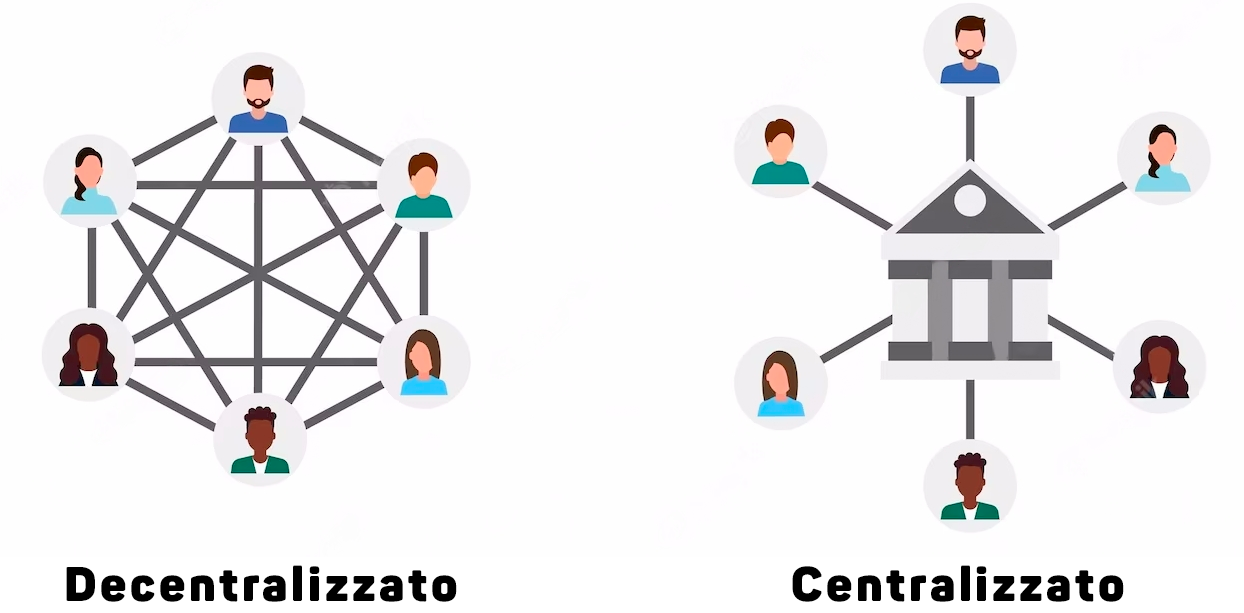
\includegraphics[width=0.79\textwidth]{images/DEFIvsCEFI.png}
    \caption{Differenza tra centralizzato e decentralizzato}
    \label{fig:defivscefi}
\end{figure}

Sono molteplici le ragioni che rendono necessario un nuovo modello di business, in grado di fornire un ambiente consono alle esigenze di venditori e acquirenti senza la necessità di un intermediario. 

Questo progetto si propone di risolvere il problema presentato, creando un marketplace decentralizzato basato su blockchain.
\chapter{Stato dell'arte}
\label{sec:state_of_the_art}

All'interno di questa sezione verranno esaminati i concetti e le tecnologie che sono alla base del progetto.
Sarà approfondita la definizione di marketplace, includendo una distinzione tra marketplace centralizzati e decentralizzati accompagnata da un'analisi dettagliata dei loro ecosistemi. Successivamente si procederà all'analisi delle tecnologie blockchain, concentrandosi sulle loro caratteristiche principali e approfondendo la blockchain Ethereum.

\section{Marketplace}
Con il termine \textit{marketplace} ci si riferisce ad un qualsiasi luogo che facilita lo scambio di beni e servizi tra acquirenti e venditori.
I marketplace possono essere fisici, come ad esempio i mercati, oppure virtuali, come i siti di e-commerce. 
Essi differiscono da negozi online tradizionali in quanto non vendono direttamente i prodotti, ma fungono da intermediari. \cite{def-marketplace}

Questo meccanismo permette di creare un ecosistema in cui i venditori sono in grado di raggiungere un pubblico più ampio, 
mentre gli acquirenti possono confrontare i prezzi e le caratteristiche dei prodotti offerti da diversi venditori. \cite{def-marketplace}

I marketplace \textit{online} si classificano in due categorie principali: \cite{bluecart-types-of-marketplaces}

\begin{itemize}
    \item \textit{Centralizzati}: marketplace in cui un'azienda o un gruppo gestisce l'intera piattaforma, inclusi i pagamenti e la gestione dei prodotti. 
    \item \textit{Decentralizzati}: marketplace che operano in una rete \textit{peer-to-peer} e quindi senza un intermediario. 
\end{itemize}

I \textit{marketplace centralizzati} sono modelli di business che attualmente presentano una dominanza nel panorama commerciale online. Questo modello è composto da un'entità centrale che gioca un ruolo fondamentale nella gestione, supervisione e facilitazione dell'intero ecosistema. 
Il suo ruolo principale è quello di fornire un'infrastruttura consolidata nella quale avvengono le transazioni commerciali. \cite{def-centralized-marketplace}

Tutti i partecipanti, sia i venditori che gli acquirenti, devono registrarsi e autenticarsi con l'entità centrale per poter utilizzare il servizio offerto. Il loro coinvolgimento include la necessità di riporre \textit{fiducia} verso l'entità centralizzata, affidandole i propri dati personali e le proprie informazioni sensibili, come dati di pagamento e dati anagrafici. \cite{def-centralized-marketplace}

Un aspetto principale di questo modello di business è la presenza di commissioni sulle vendite, esse vengono applicate per coprire i costi di gestione della piattaforma e per generare un profitto. 

Come già anticipato, questo modello di business è attualmente dominante, allo stesso tempo però presenta alcune limitazioni. La concentrazione del potere in un'unica entità può portare a preoccupazioni legate alla sicurezza e alla privacy, nonché alla gestione delle transazioni, essendo \textit{non} trasparenti. \cite{def-centralized-marketplace}

I \textit{marketplace decentralizzati} operano in una rete \textit{peer-to-peer} fornendo servizi comparabili ad un marketplace centralizzato, ma a differenza di quest'ultimo operano senza intermediario.

Essi sono comunemente associati alle tecnologie \hyperref[sec:blockchain]{\textit{Blockchain}}, in quanto possiedono un ambiente sicuro e trasparente per la gestione delle transazioni. Questo permette di migliorare, rispetto ad un sistema centralizzato, la sicurezza e la trasparenza del marketplace. L'assenza di un punto di controllo centrale riduce notevolmente il rischio di frodi e manipolazioni, poiché le transazioni vengono verificate e registrate in modo immutabile sulla blockchain. Ciò significa che gli utenti non sono costretti a riporre totale fiducia in un'entità centrale, ma possono invece confidare nella crittografia e nella matematica della blockchain stessa. \cite{def-decentralized-marketplace}

Un ulteriore confronto tra le due tipologie di marketplace dimostra che anche a livello di privacy vi sono delle differenze. Infatti, con i \textit{marketplace decentralizzati} non è necessario autenticarsi con i propri dati personali ma è sufficiente un \hyperref[sec:wallet]{\textit{wallet}} per accedere. \cite{def-decentralized-marketplace}

Di seguito, la tabella comparativa \ref{table:confronto-marketplace} mostra le principali differenze tra le due tipologie di marketplace.

\newpage

\begin{table}[H]
    \centering
    \renewcommand{\arraystretch}{1.5}
    \begin{adjustbox}{max width=1\textwidth}
        \begin{tabular}{| p{0.33\linewidth} | p{0.33\linewidth} | p{0.33\linewidth} |}
            \hline
            \rowcolor{mint-cream}
            Caratteristiche                  & Centralizzato                                                       & Decentralizzato                                      \\
            \hline
            Ruolo dell'entità centrale       & Fondamentale nella gestione e facilitazione                         & Assenza di intermediari o entità centrali            \\
            \hline
            Partecipazione e autenticazione  & Richiede la registrazione e autenticazione presso l'entità centrale & Accesso tramite wallet e crittografia Blockchain     \\
            \hline
            Fiducia e dati personali         & Necessita fiducia nell'entità centrale                              & Fiducia basata sulla crittografia e sulla Blockchain \\
            \hline
            Sicurezza, privacy e trasparenza & Preoccupazione generale riguardo alla gestione dei dati             & Potenziati dalla tecnologia Blockchain               \\
            \hline
            Gestione delle transazioni       & Gestite centralmente, spesso non trasparenti                        & Verificate e registrate in modo immutabile          \\
            \hline
        \end{tabular}
    \end{adjustbox}
    \caption{Confronto tra Marketplace Centralizzato e Decentralizzato}
    \label{table:confronto-marketplace}
\end{table}

\section{Web 3.0}
\label{sec:web3}
Il termine Web 3.0 è stato coniato dal cofondatore di Ethereum Gavin Wood nel 2014. Wood idealizzò una soluzione per uno dei principali problemi del Web tradizionale: troppa \textit{fiducia} è richiesta. La maggior parte dei siti tradizionali, come i \textit{marketplace centralizzati}, si basano sul presupposto di porre fiducia che una serie di compagnie private agisca nel pieno interesse pubblico. \cite{web3-ethereum}

Le caratteristiche che contraddistinguono Web 3.0, o più semplicemente Web3, sono:
\begin{itemize}
    \item Decentralizzazione: al posto di grandi aree di Internet controllate da entità centralizzate, la proprietà di Web3 è distribuita tra i suoi creatori e i suoi utenti.
    \item Non prevede permessi e privilegi: l'accesso a Web3 è uguale per tutti coloro che vogliono accedervi, nessuno escluso.
    \item Prevede nativamente i pagamenti: invece di appoggiarsi a banche ed elaboratori di pagamento, Web3 utilizza criptovalute per spendere e inviare denaro online.
    \item Non si basa sulla fiducia: opera usando incentivi e meccanismi economici invece di affidarsi a terze parti fidate.
\end{itemize}
Ciò che rende importante il Web3 è la possibilità di possedere risorse digitali in maniera diretta, senza bisogno di intermediari, oltre a garantire resistenza alla censura da parte di entità centralizzate.
Il Web3 necessita di una tecnologia distribuita per poter funzionare: \textit{Blockchain}. \cite{web3-ethereum}

\section{Blockchain}
\label{sec:blockchain-module}

Nel seguente capitolo viene descritto in maniera più approfondita il componente \textit{Blockchain}. In particolare, vengono analizzati gli smart contracts, i quali sono stati sviluppati utilizzando il framework \textit{Hardhat} e il linguaggio di programmazione \textit{Solidity} ma anche gli script utilizzati per l'automazione di alcune operazioni, i test effettuati e le possibili alternative.

\subsection{Smart contracts}
\label{sec:smart-contract-shopychange}

Per il corretto funzionamento del marketplace, sono stati sviluppati diversi smart contracts. In particolare, il contratto principale è \textit{ShopychangeMarketplace}, il quale si occupa di gestire la creazione, modifica, cancellazione e acquisto di una vendita. Inoltre, gestisce le \textit{royalty} e fornisce delle funzionalità di controllo per gli amministratori.

In aggiunta, il contratto \textit{ERC721 Factory} offre la possibilità di creazione di nuovi smart contracts di tipo \textit{ERC721} utilizzando un \textit{template} chiamato \textit{Boilerplate ERC721}. 

Infine, lo \textit{smart contract} \textit{Storage} viene utilizzato dagli utenti che non hanno necessità di creare una nuova collezione ma di generare un singolo asset.  

Nei prossimi capitoli verranno analizzati in dettaglio i contratti che compongono il marketplace. Di seguito, a figura \ref{fig:legenda}, è osservabile una legenda per la comprensione dei diagrammi.
\begin{figure}[H]
    \centering
    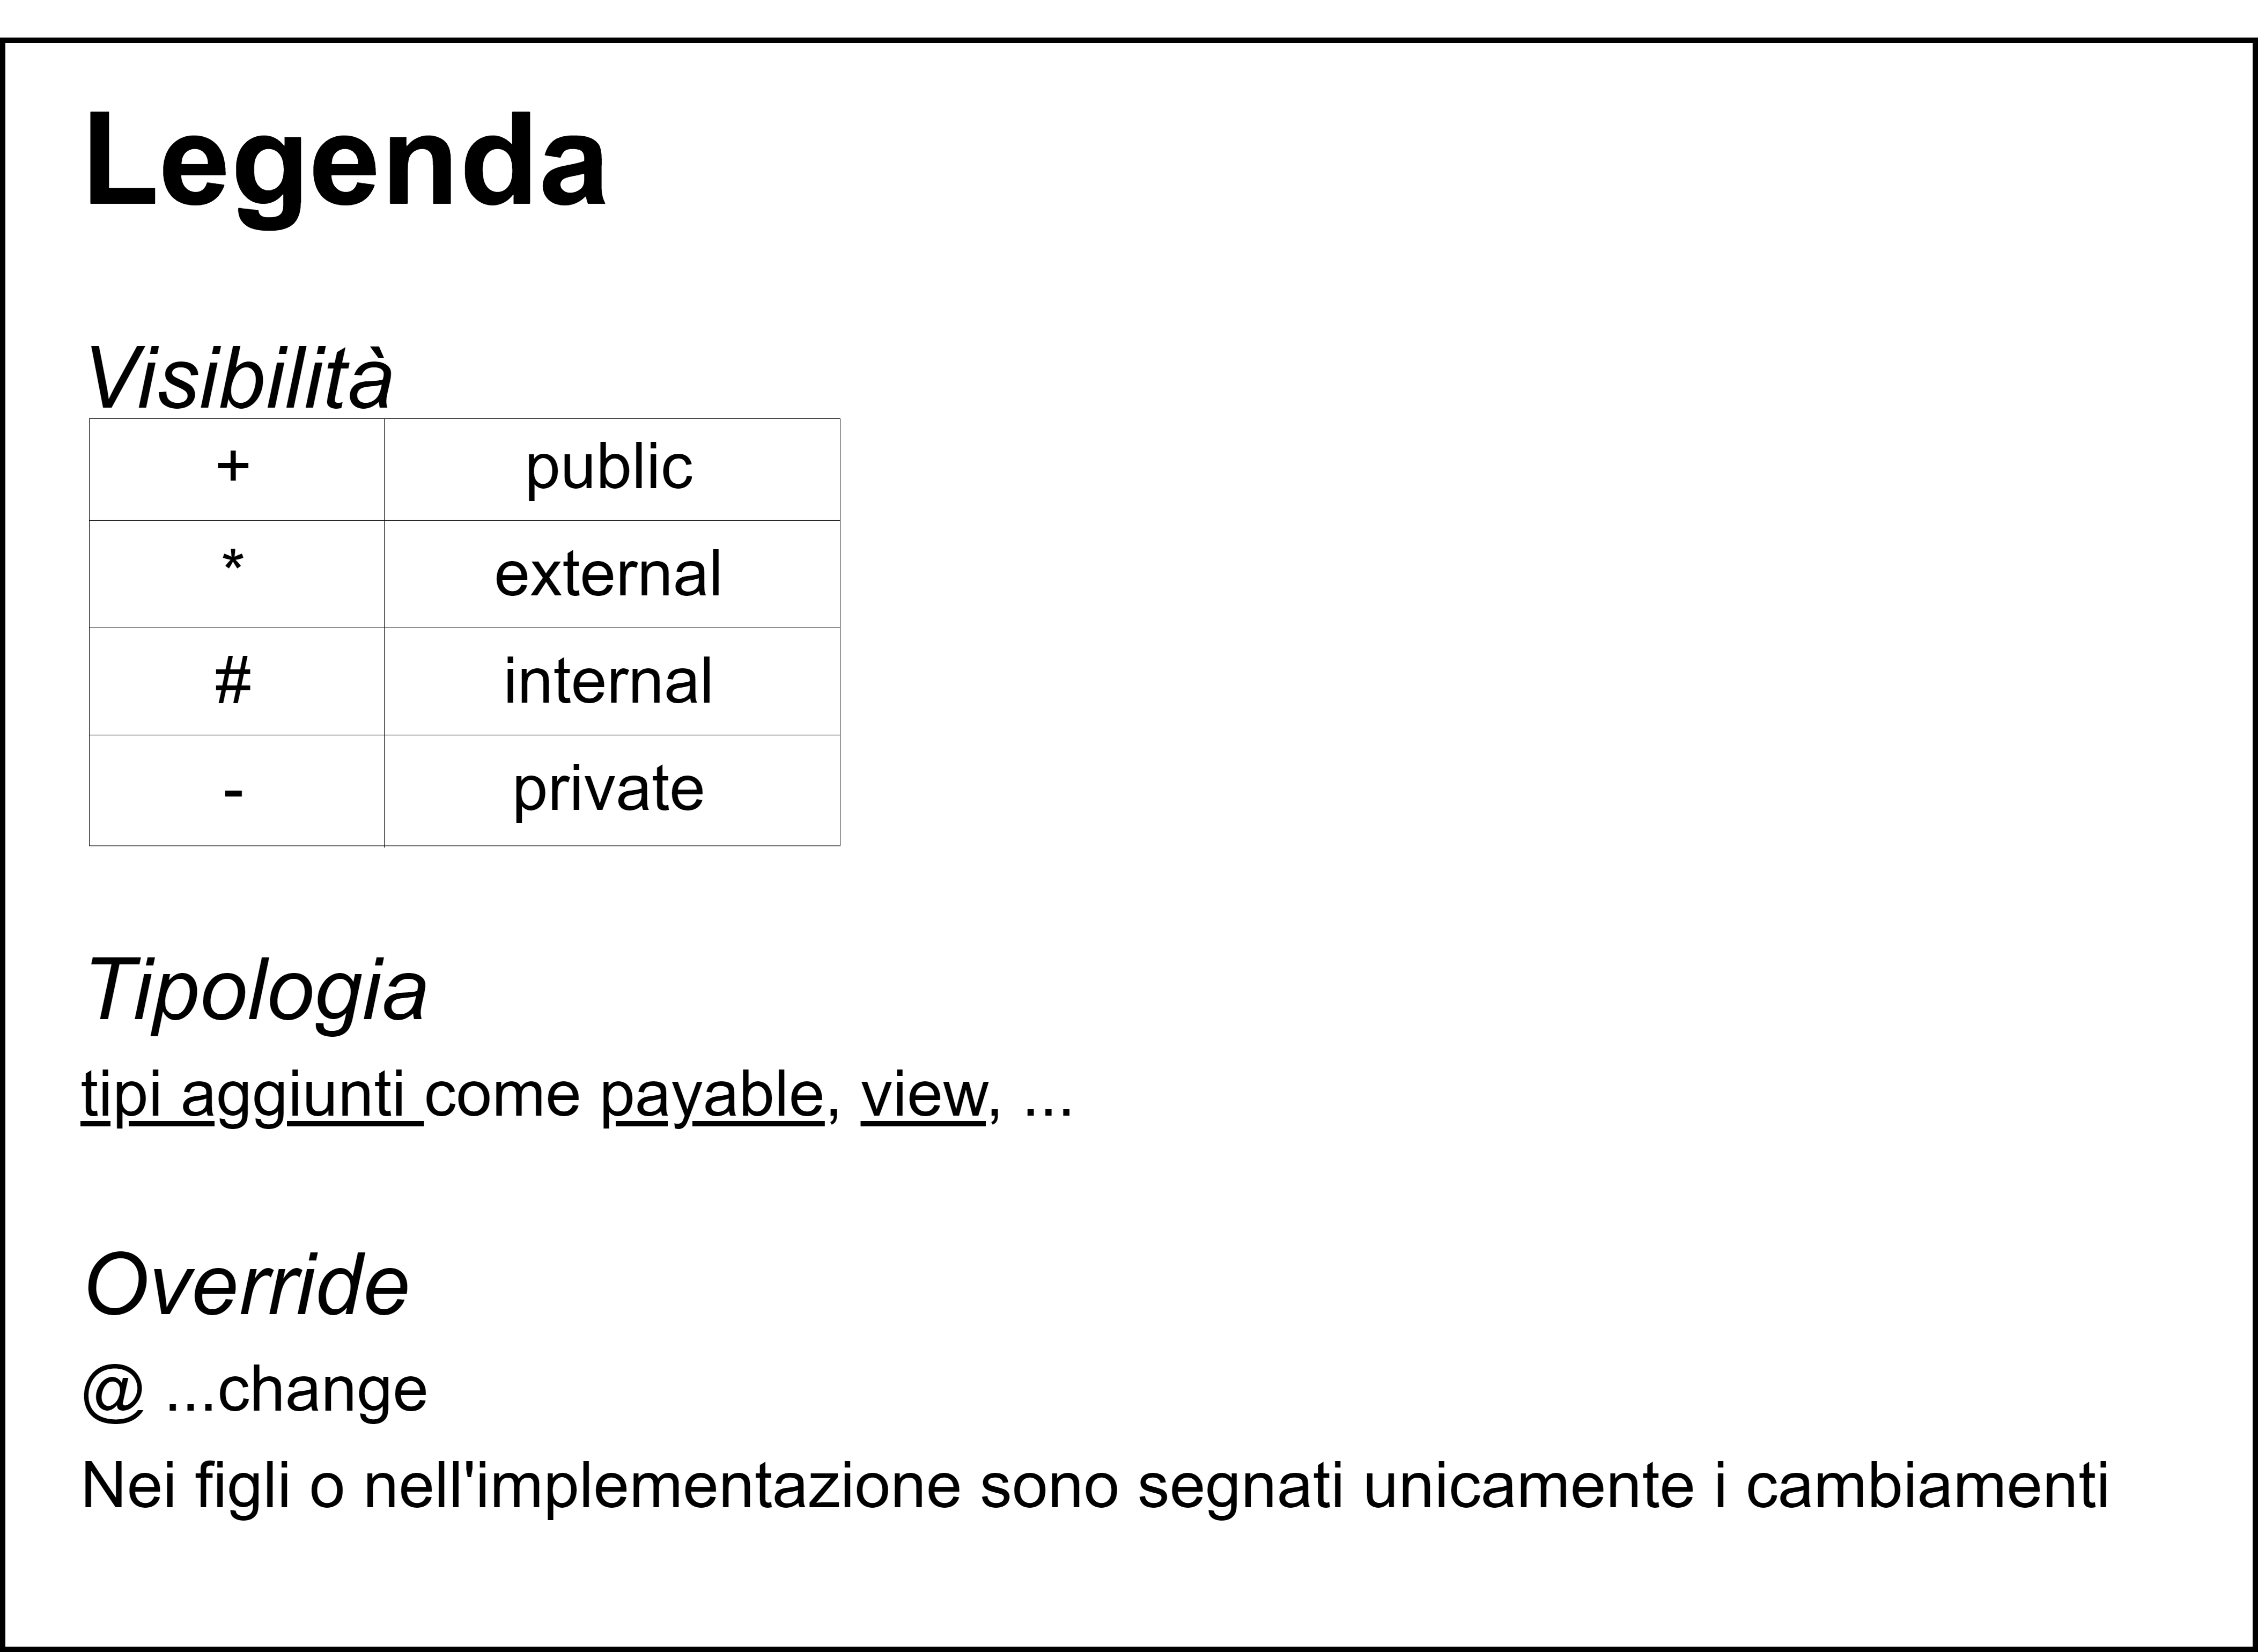
\includegraphics[width=0.8\textwidth]{images/blockchainContracts/LegendaBordo.png}
    \caption{Legenda Smart contracts}
    \label{fig:legenda}
\end{figure}

\subsubsection{Marketplace}

Il contratto \textit{core} del marketplace è \textit{ShopychangeMarketplace}. Per la sua realizzazione è stato deciso di utlizzare un approccio simile allo standard \textit{ERC721}, ovvero separando la logica in più contratti per facilitare la manutenzione, comprensione e testabilità del codice. Inoltre, grazie alla struttura a modelli è possibile decidere quali funzionalità abilitare o meno. Il contratto \textit{ShopychangeMarketplace} possiede tutte le funzionalità. La figura \ref{fig:marketplaceContract} mostra il diagramma UML del contratto.

\begin{figure}[H]
    \centering
    \includegraphics[width=1\textwidth]{images/blockchainContracts/ShopychangeMarketplaceReduced.png}
    \caption{Diagramma smart contract ShopychangeMarketplace}
    \label{fig:marketplaceContract}
\end{figure}


\paragraph{Fundamental}

Come si può osservare dalla figura \ref{fig:marketplaceFundamental}, il contratto \textit{MarketplaceFundamental} eredita dall'interfaccia \textit{IMarketplaceFundamental}. Questa interfaccia definisce le funzionalità obbligatorie del contratto \textit{Fundamental}, ovvero la creazione e acquisto di una vendita. Le informazioni relative alla vendita sono salvate in una struttura dati chiamata \textit{Sale}. Più in dettaglio, la struttura dati contiene le seguenti informazioni:

\begin{itemize}
    \item \textit{contractAddress}: indirizzo del contratto che rappresenta la collezione
    \item \textit{tokenId}: identificativo dell'asset all'interno della collezione
    \item \textit{price}: prezzo di vendita
    \item \textit{seller}: indirizzo del venditore
    \item \textit{status}: stato della vendita, può essere \textit{None} = 0 (Non presente nel marketplace), \textit{Cancelled} = 1 (Cancellata), \textit{Sold} = 2 (Venduta), \textit{Listed} = 3 (In vendita)
\end{itemize}

Gli attributi \textit{\_sales} e \textit{\_salesIds} presenti nel contratto \textit{MarketplaceFundamental} sono utilizzati per mantenere le informazioni relative alle vendite. In maniera più approfondita, \textit{\_sales} è una \textit{map} che associa ad ogni identificativo di una vendita la struttura dati \textit{Sale}. Mentre, \textit{\_salesIds} è un array che contiene gli identificativi delle vendite presenti nel marketplace. L'id in formato \textit{bytes32} è generato crittografando l'indirizzo del contratto e l'identificativo dell'asset, creando così un valore univoco per ogni vendita. L'id generato è ottenibile utilizzando la funzione \textit{getKey}. 

Nel momento in cui avviene la creazione di una vendita, lo smart contract controllerà che le informazioni fornite siano valevoli e che il chiamante sia effettivamente il possessore dell'asset. Un processo simili avviene anche all'acquisto del token, dove il contratto verifica che il \textit{seller} sia ancora il possessore. Maggiori dettagli su questa possibile situazioni sono presenti nel capitolo \hyperref[sec:controllo-integrita-nft-in-vendita]{\textit{Controllo integrità NFT in vendita}}.

Nel momento in cui avviene un acquisto, il metodo \textit{buy} eseguirà \textit{payShares}, questo meccanismo permetterà ai contratti figli di poter gestire le \textit{royalty} in maniera personalizzata. Maggiori informazioni nei capitoli \hyperref[sec:marketplace-earnable]{\textit{Earnable}} e \hyperref[sec:marketplace-royalty-applicable]{\textit{RoyaltyApplicable}}.

Infine, il contratto presenta alcune funzioni di tipo \textit{view}, le quali permettono di ottenere le vendite presenti nel marketplace.

\begin{figure}[H]
    \centering
    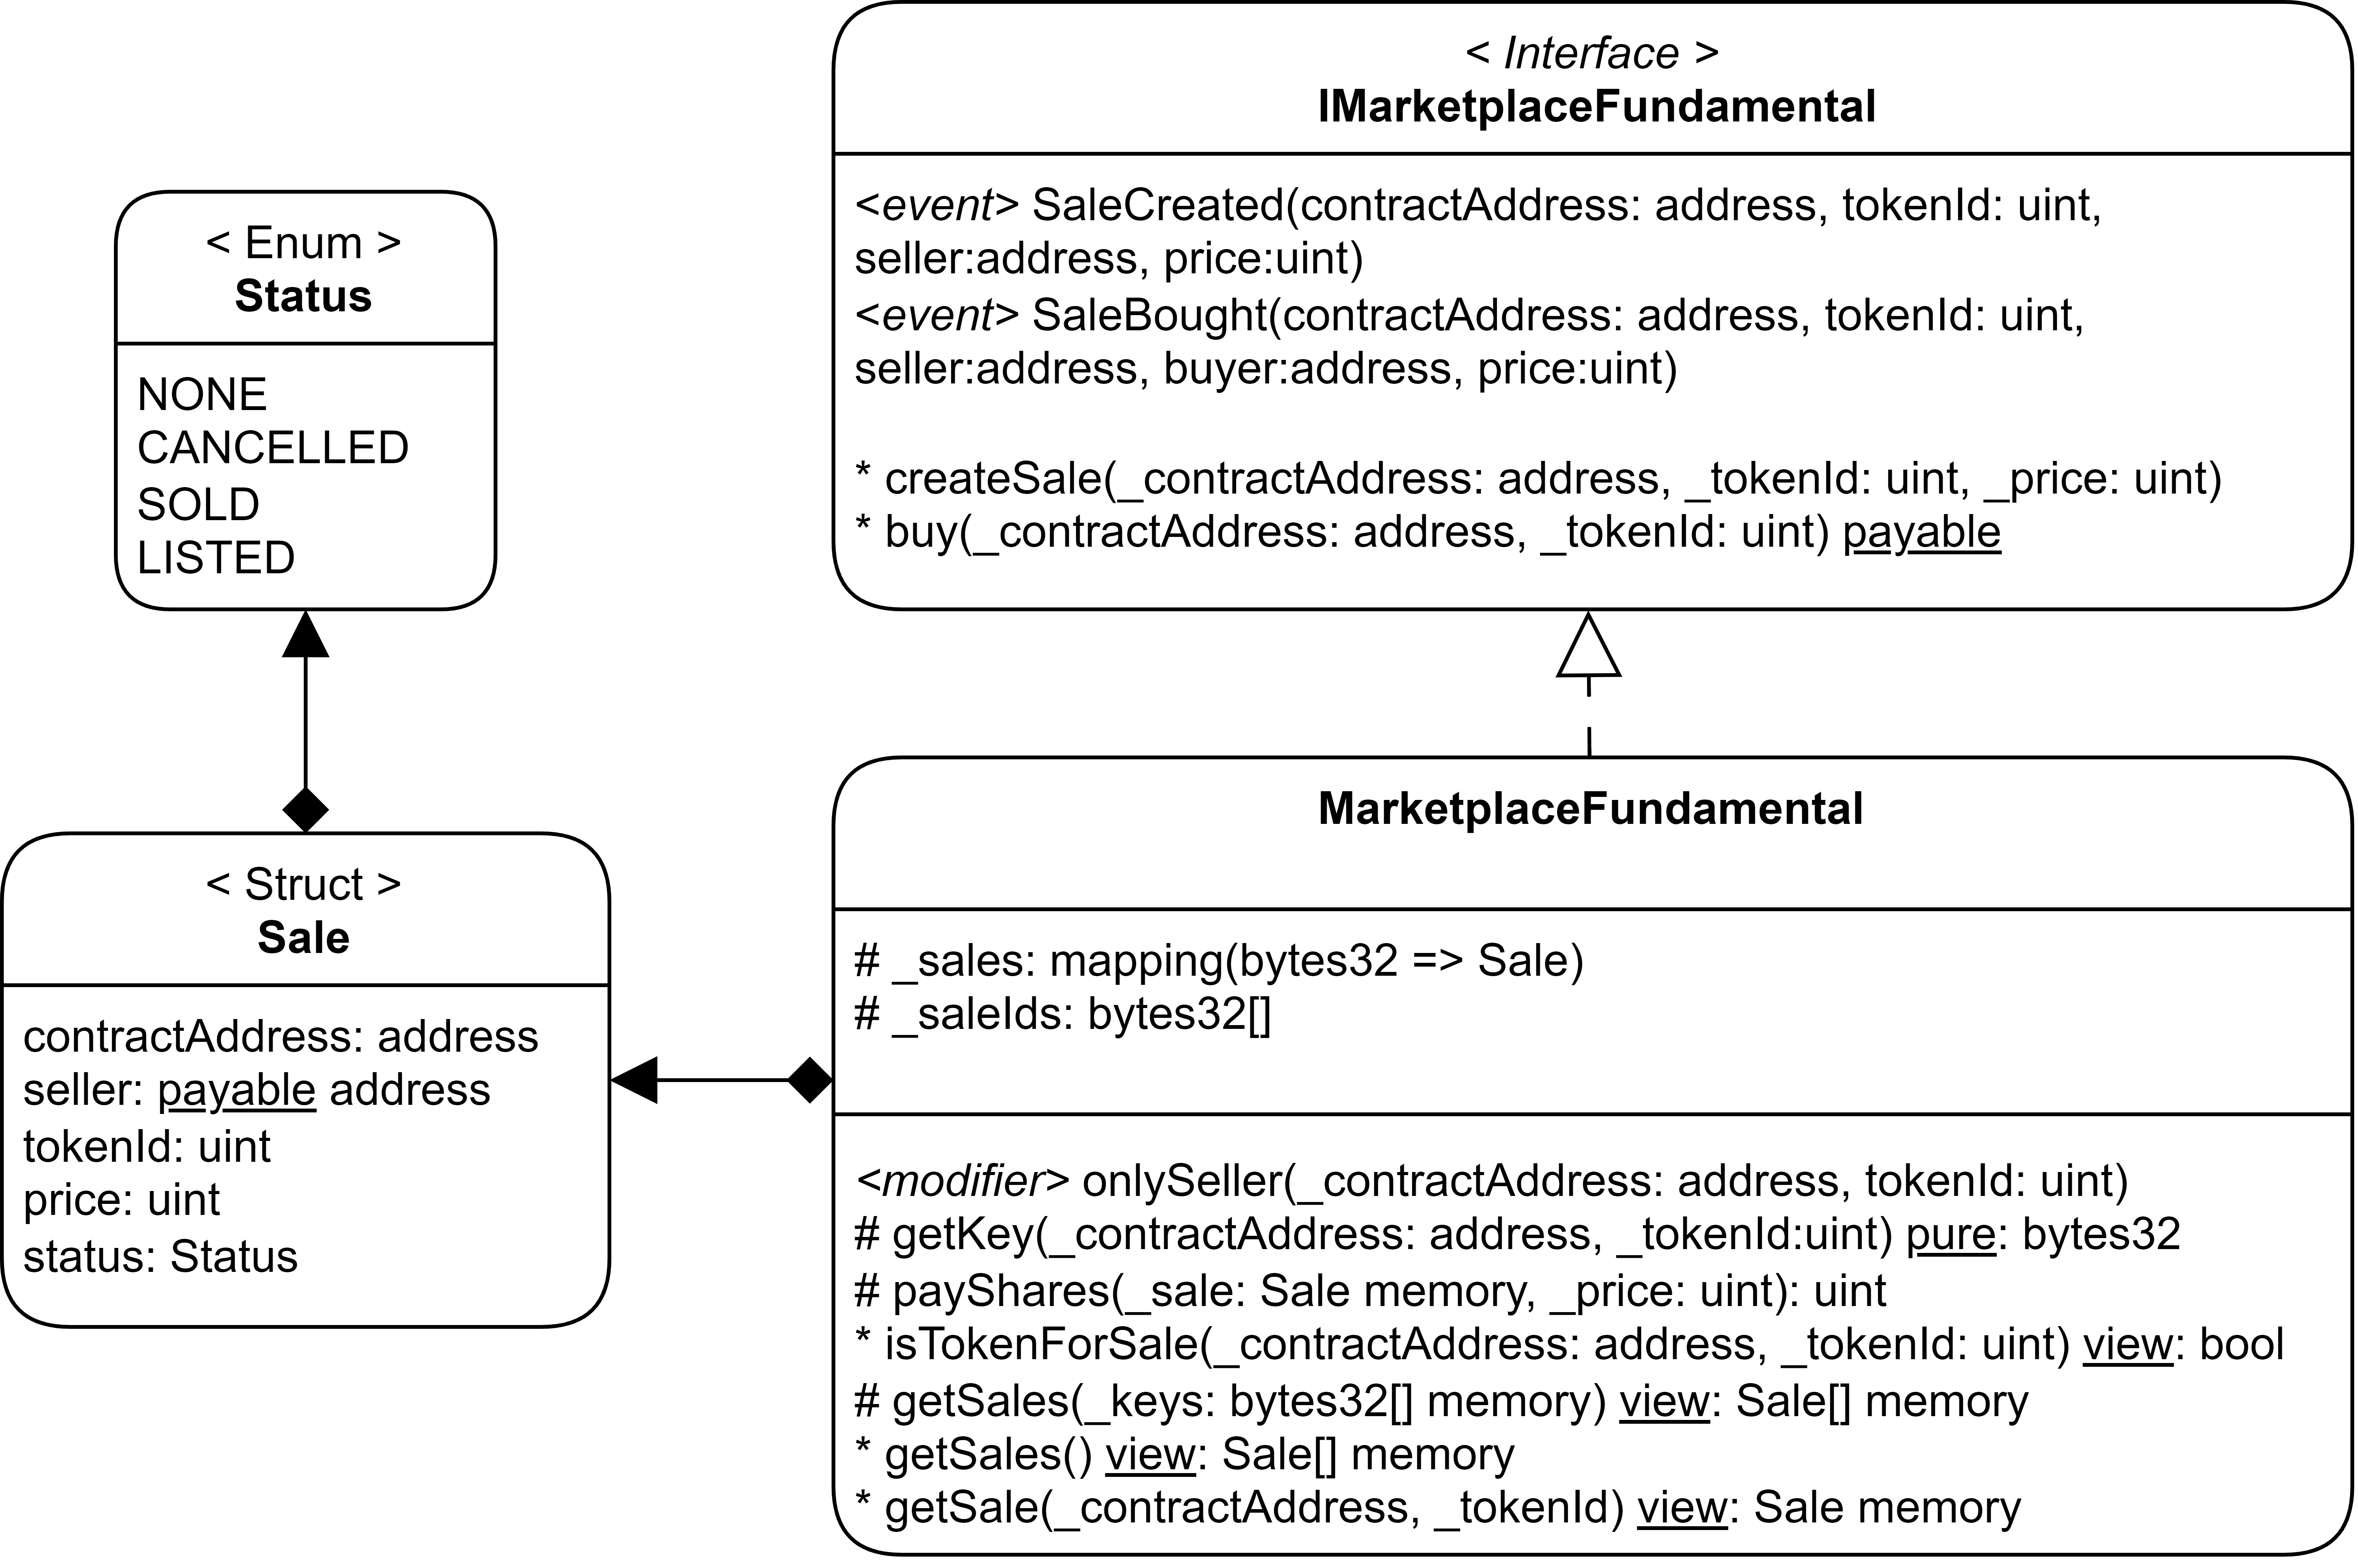
\includegraphics[width=1\textwidth]{images/blockchainContracts/MarketplaceFundamental.png}
    \caption{Marketplace Fundamental}
    \label{fig:marketplaceFundamental}
\end{figure}



\paragraph{Cancellable}
L'estensione \textit{Cancellable} permette la cancellazione di una vendita in corso. Nello specifico, il contratto \textit{MarketplaceCancellable} eredita da \textit{IMarketplaceCancellable} e \textit{MarketplaceFundamental}. Come visibile in figura \ref{fig:marketplaceCancellable} il contratto presenta la funzione \textit{cancelSale}, la quale è utilizzabile unicamente dal possessore dell'asset o dall'amministratore.

\begin{figure}[H]
    \centering
    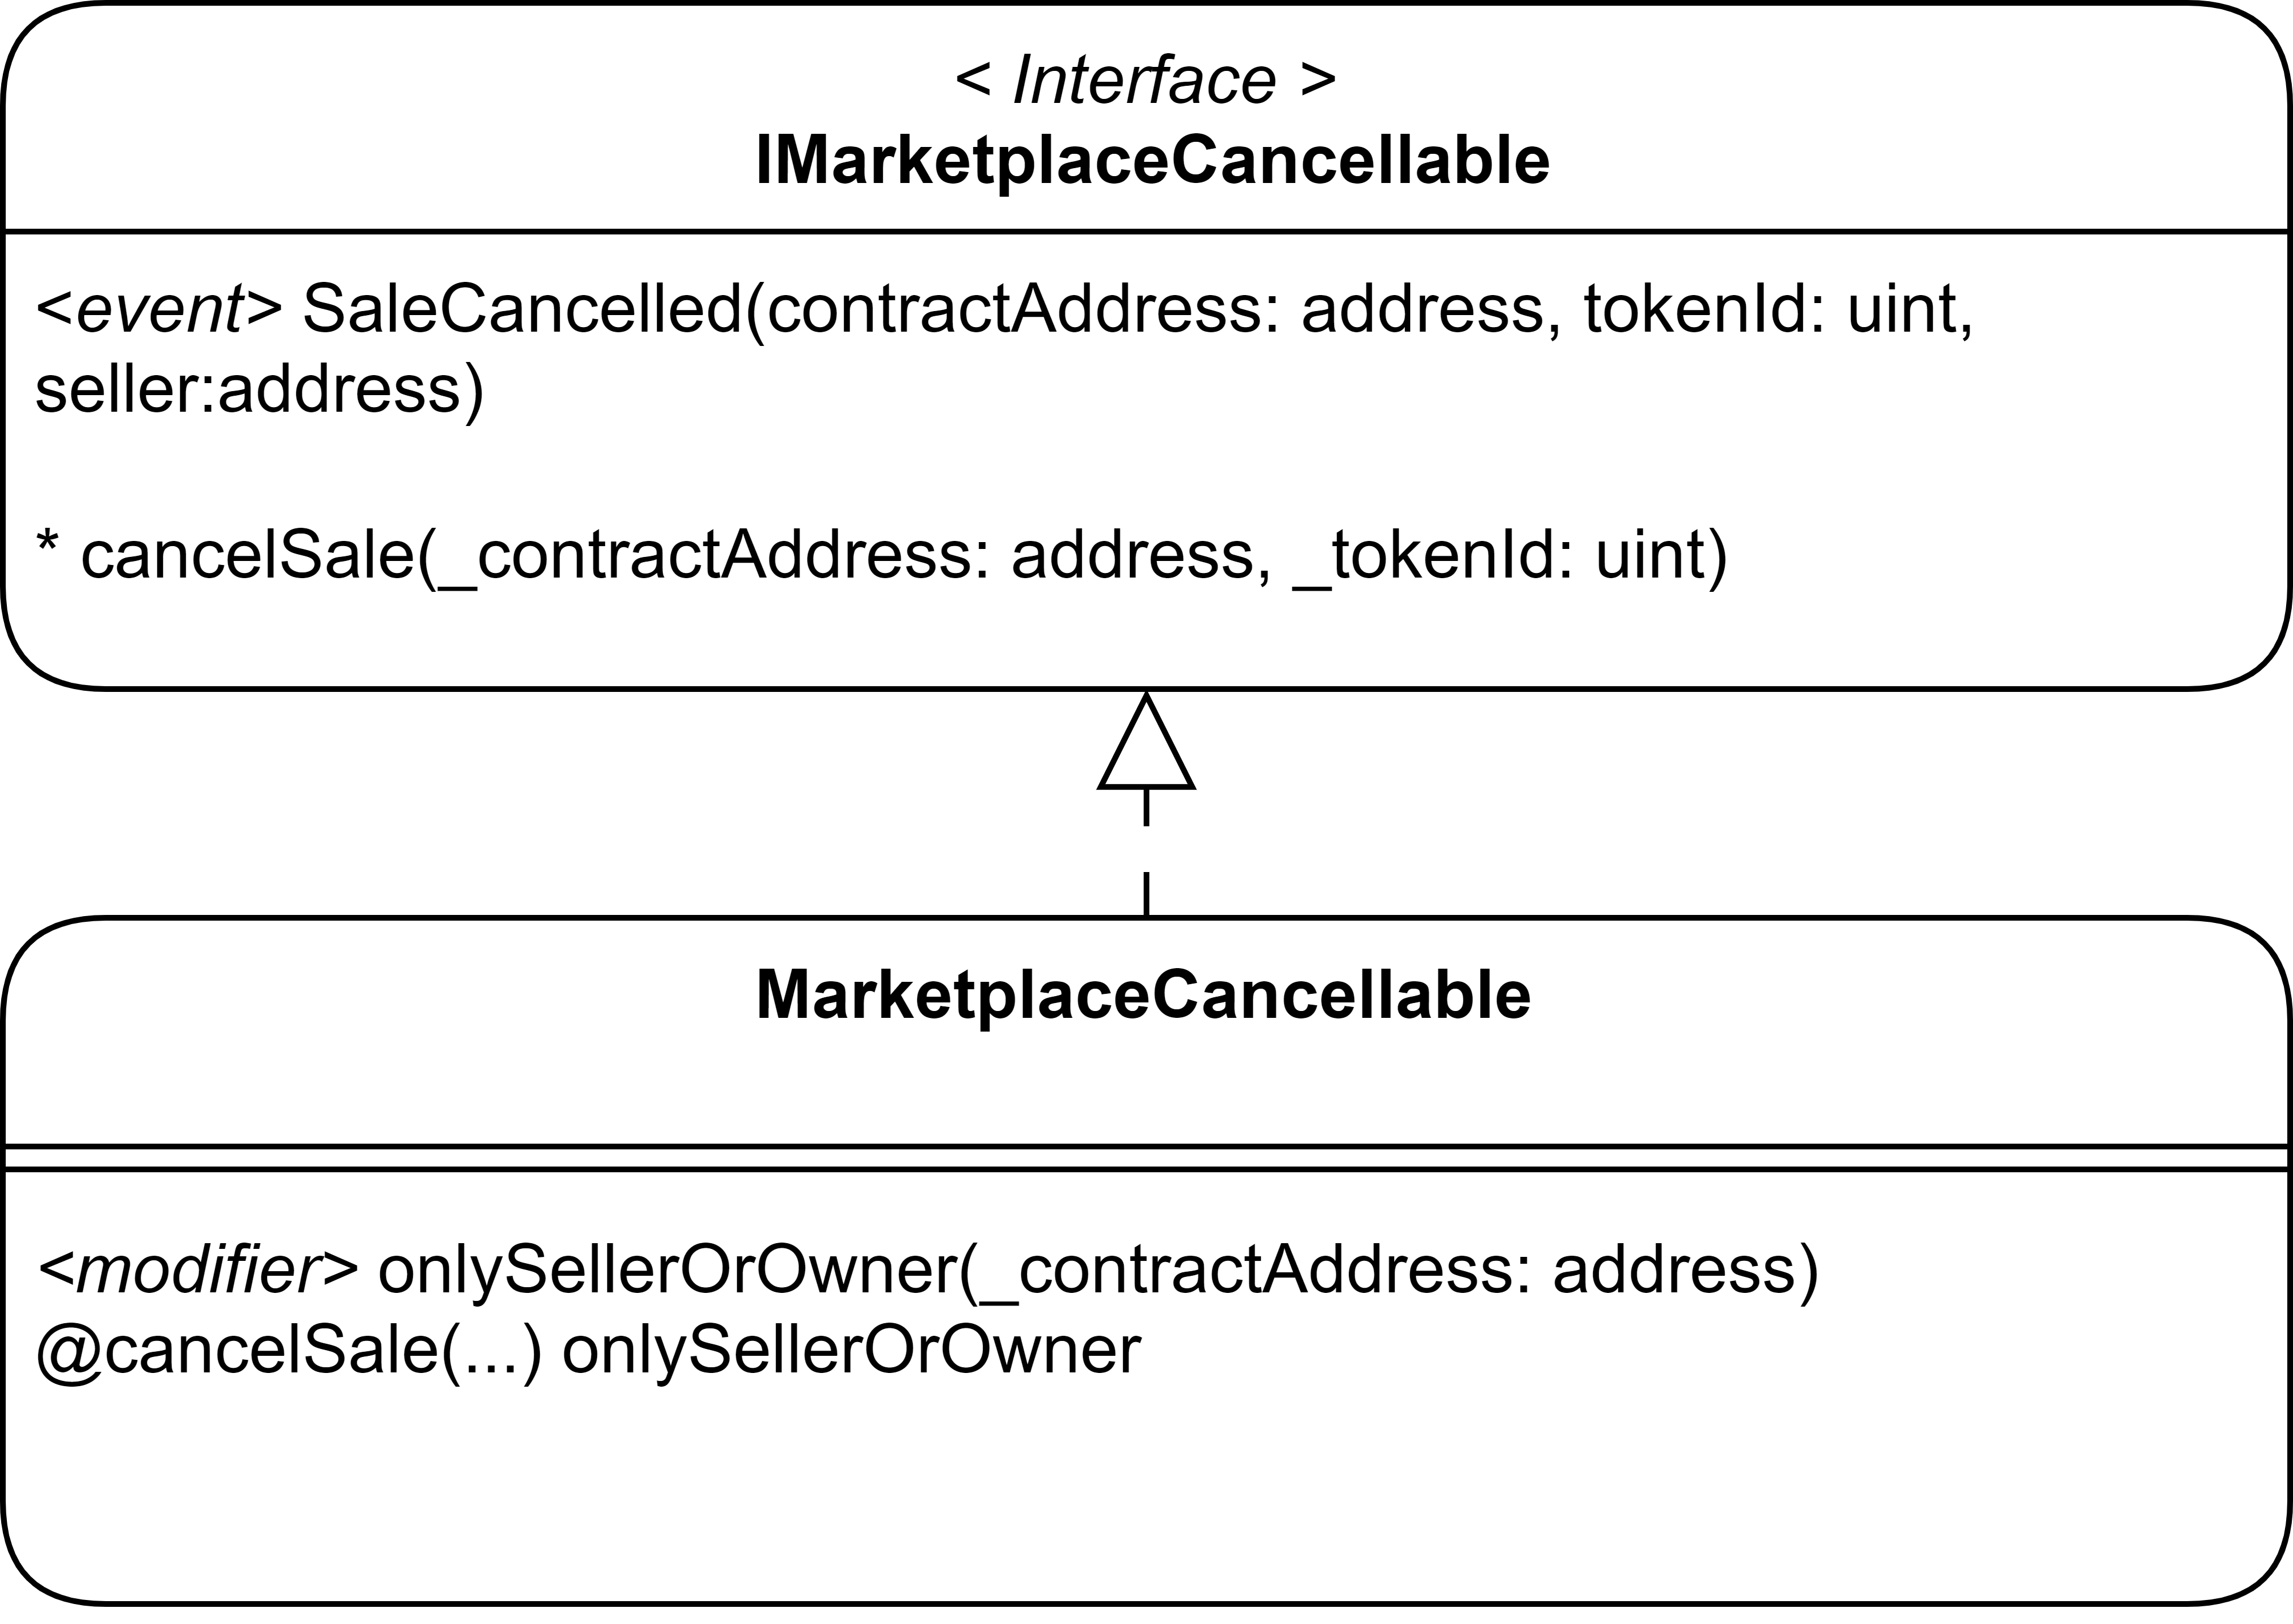
\includegraphics[width=0.7\textwidth]{images/blockchainContracts/MarketplaceCancellable.png}
    \caption{Marketplace Cancellable}
    \label{fig:marketplaceCancellable}
\end{figure}

\paragraph{Modifiable}
Il contratto \textit{MarketplaceModifiable} estende \textit{IMarketplaceModifiable} e \textit{IMarketplaceCancellable}. La sua funzione è quella di consentire la modifica del prezzo di vendita di un asset. Questa operazione è eseguibile unicamente dal possessore dell'asset, come visibile in figura \ref{fig:marketplaceModifiable}.

\begin{figure}[H]
    \centering
    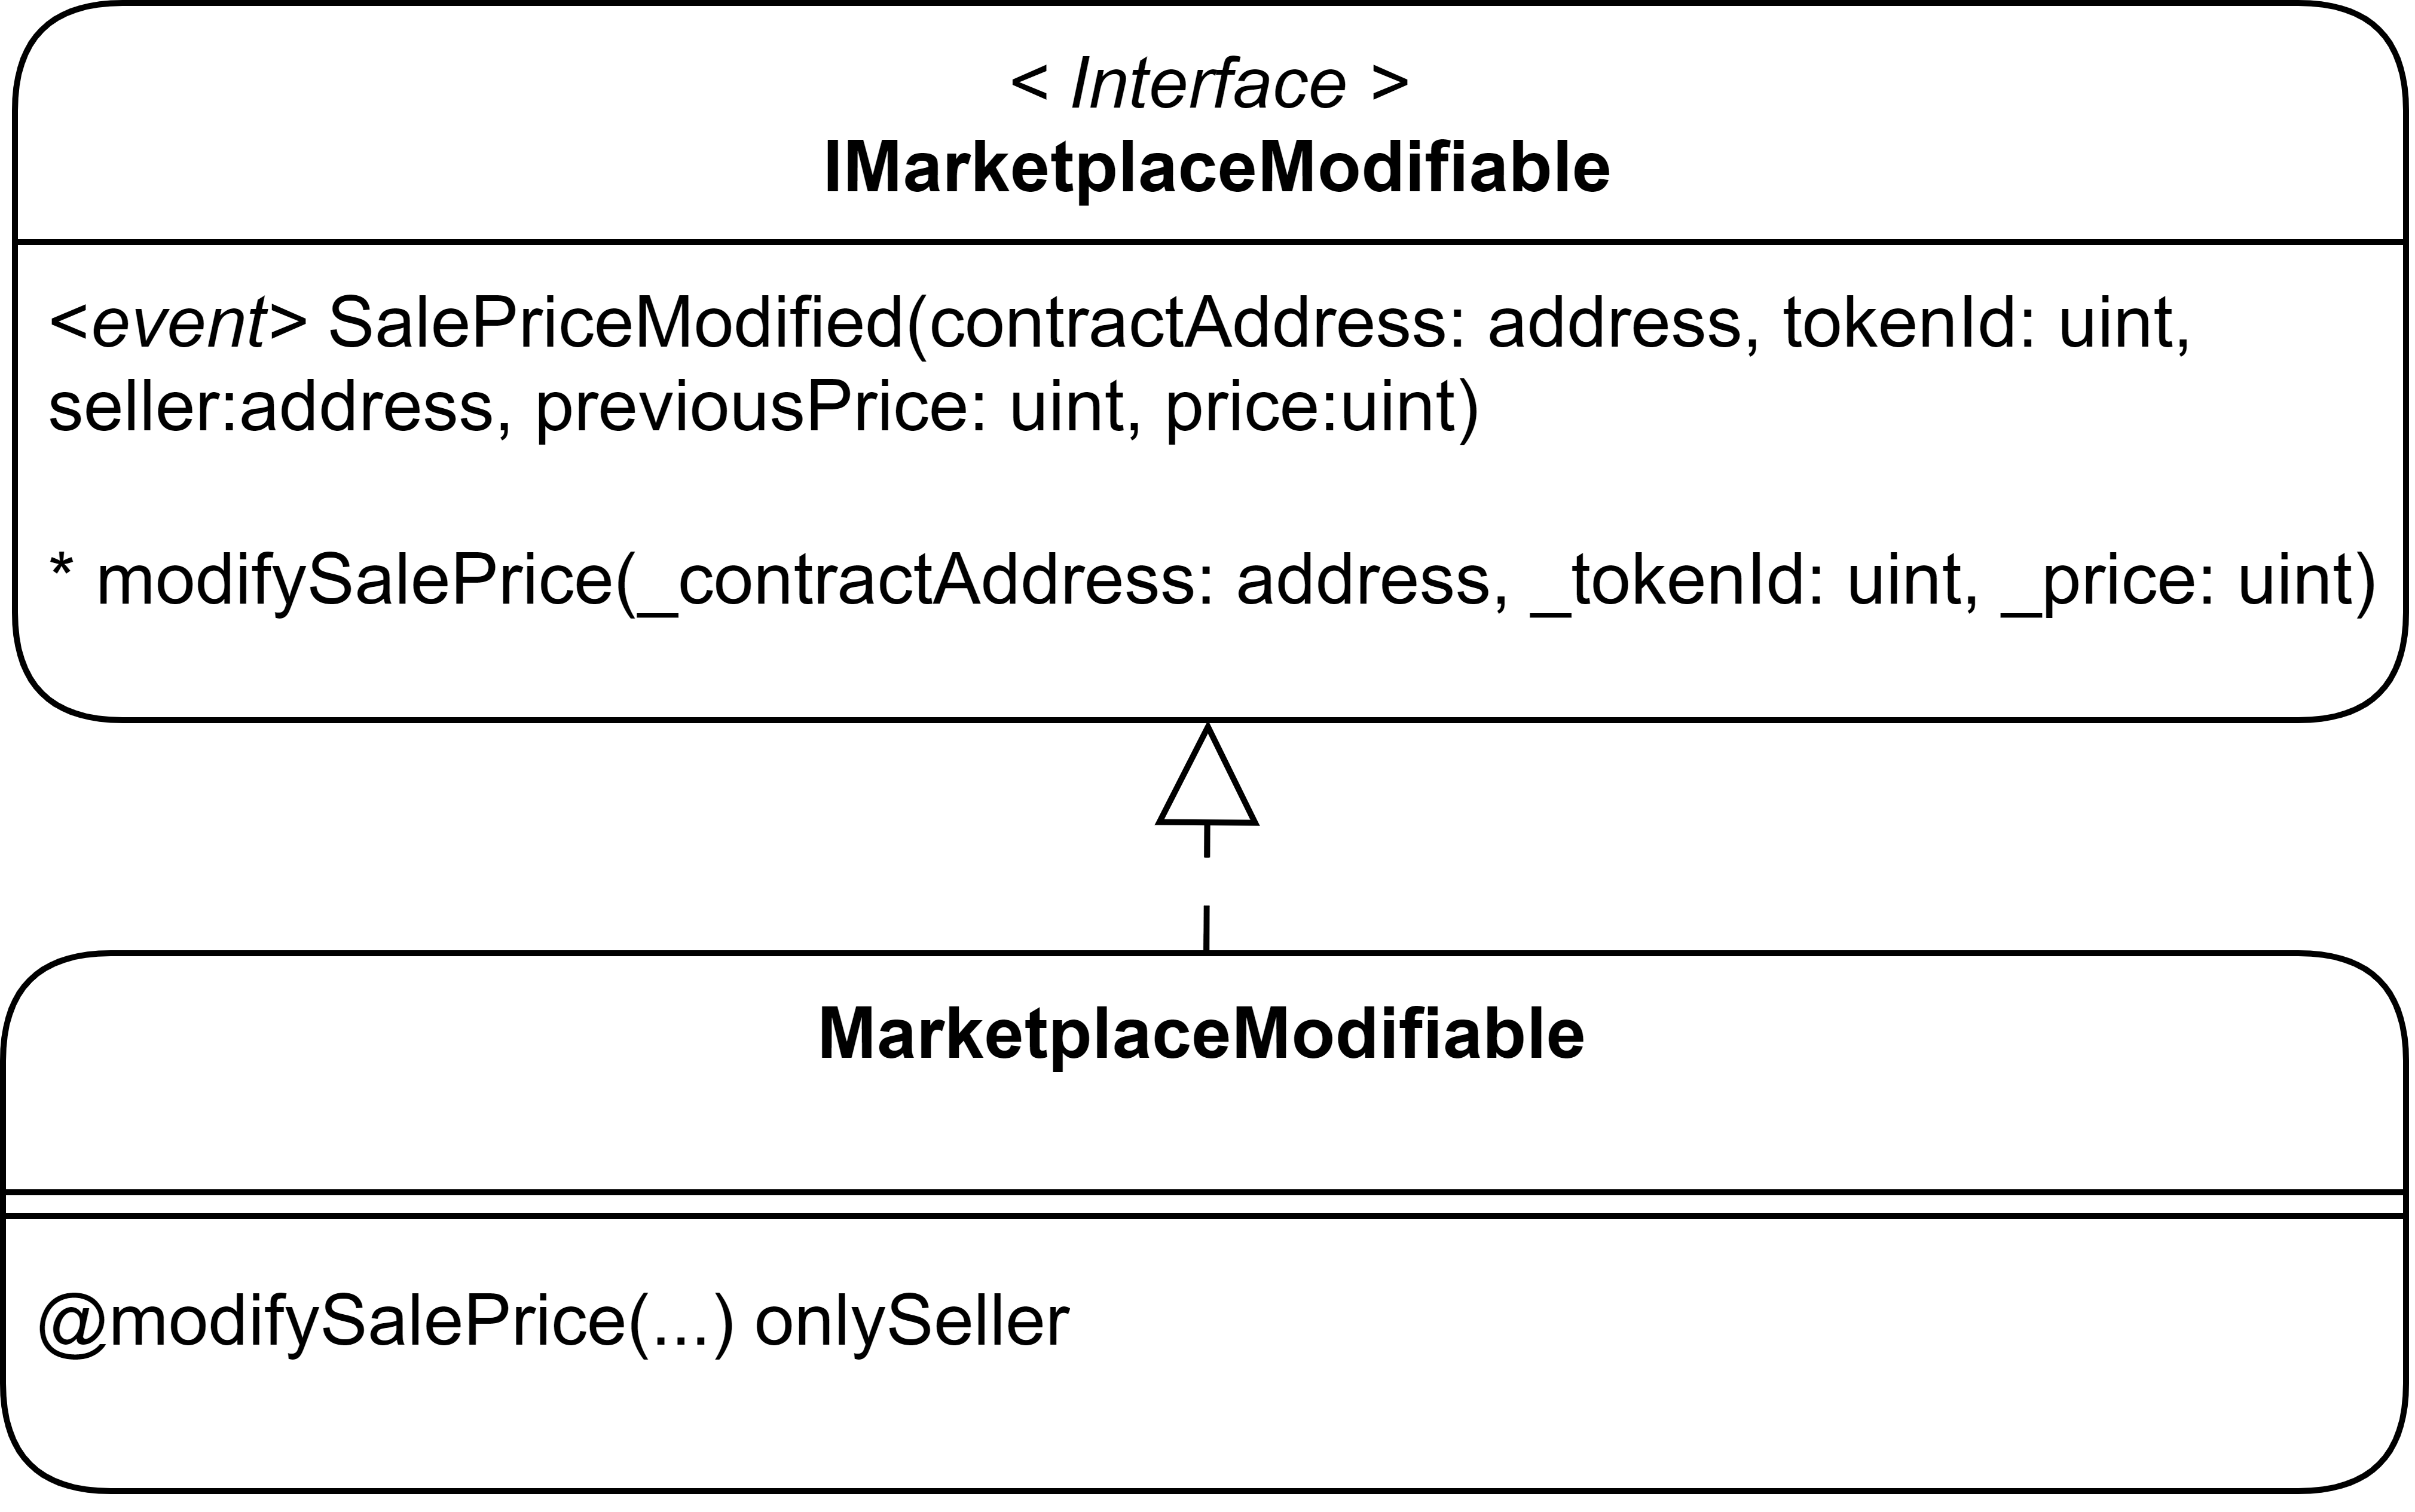
\includegraphics[width=0.7\textwidth]{images/blockchainContracts/MarketplaceModifiable.png}
    \caption{Marketplace Modifiable}
    \label{fig:marketplaceModifiable}
\end{figure}

\paragraph{Earnable}
\label{sec:marketplace-earnable}

Questo contratto consente il collezionamento di royalty a favore del marketplace per ogni acquisto effettuato. Come visibile in figura \ref{fig:marketplaceEarnable}, il contratto contiene il metodo \textit{receiver}, ovvero uno speciale metodo che permette al contratto di ricevere \textit{ETH}. La possibilità di collezionare le royalty è data dal metodo \textit{payShares}, il quale viene chiamato all'interno contratto \textit{MarketplaceFundamental}  nel momento in cui avviene un acquisto. 

Più in dettaglio, effettuando l'\textit{override} del metodo \textit{payShares}, che sarà chiamato dal metodo \textit{buy}, avviene una divisione del prezzo di vendita in base al valore presente nell'attributo \textit{royalty}. Questo valore rappresenta la percentuale di royalty che il marketplace riceverà per ogni acquisto, esso è un \textit{uint16} in quanto rappresenta un valore percentuale in \textit{basis point} (il valore 1 corrisponde allo 0.01\%, mentre il valore 10000 rappresenta il 100\%). In aggiunta, sono presenti alcune funzionalità di \textit{get} e \textit{set} per modificare il valore percentuale, nonchè diversi metodi per ritirare il saldo del contratto. 

\begin{figure}[H]
    \centering
    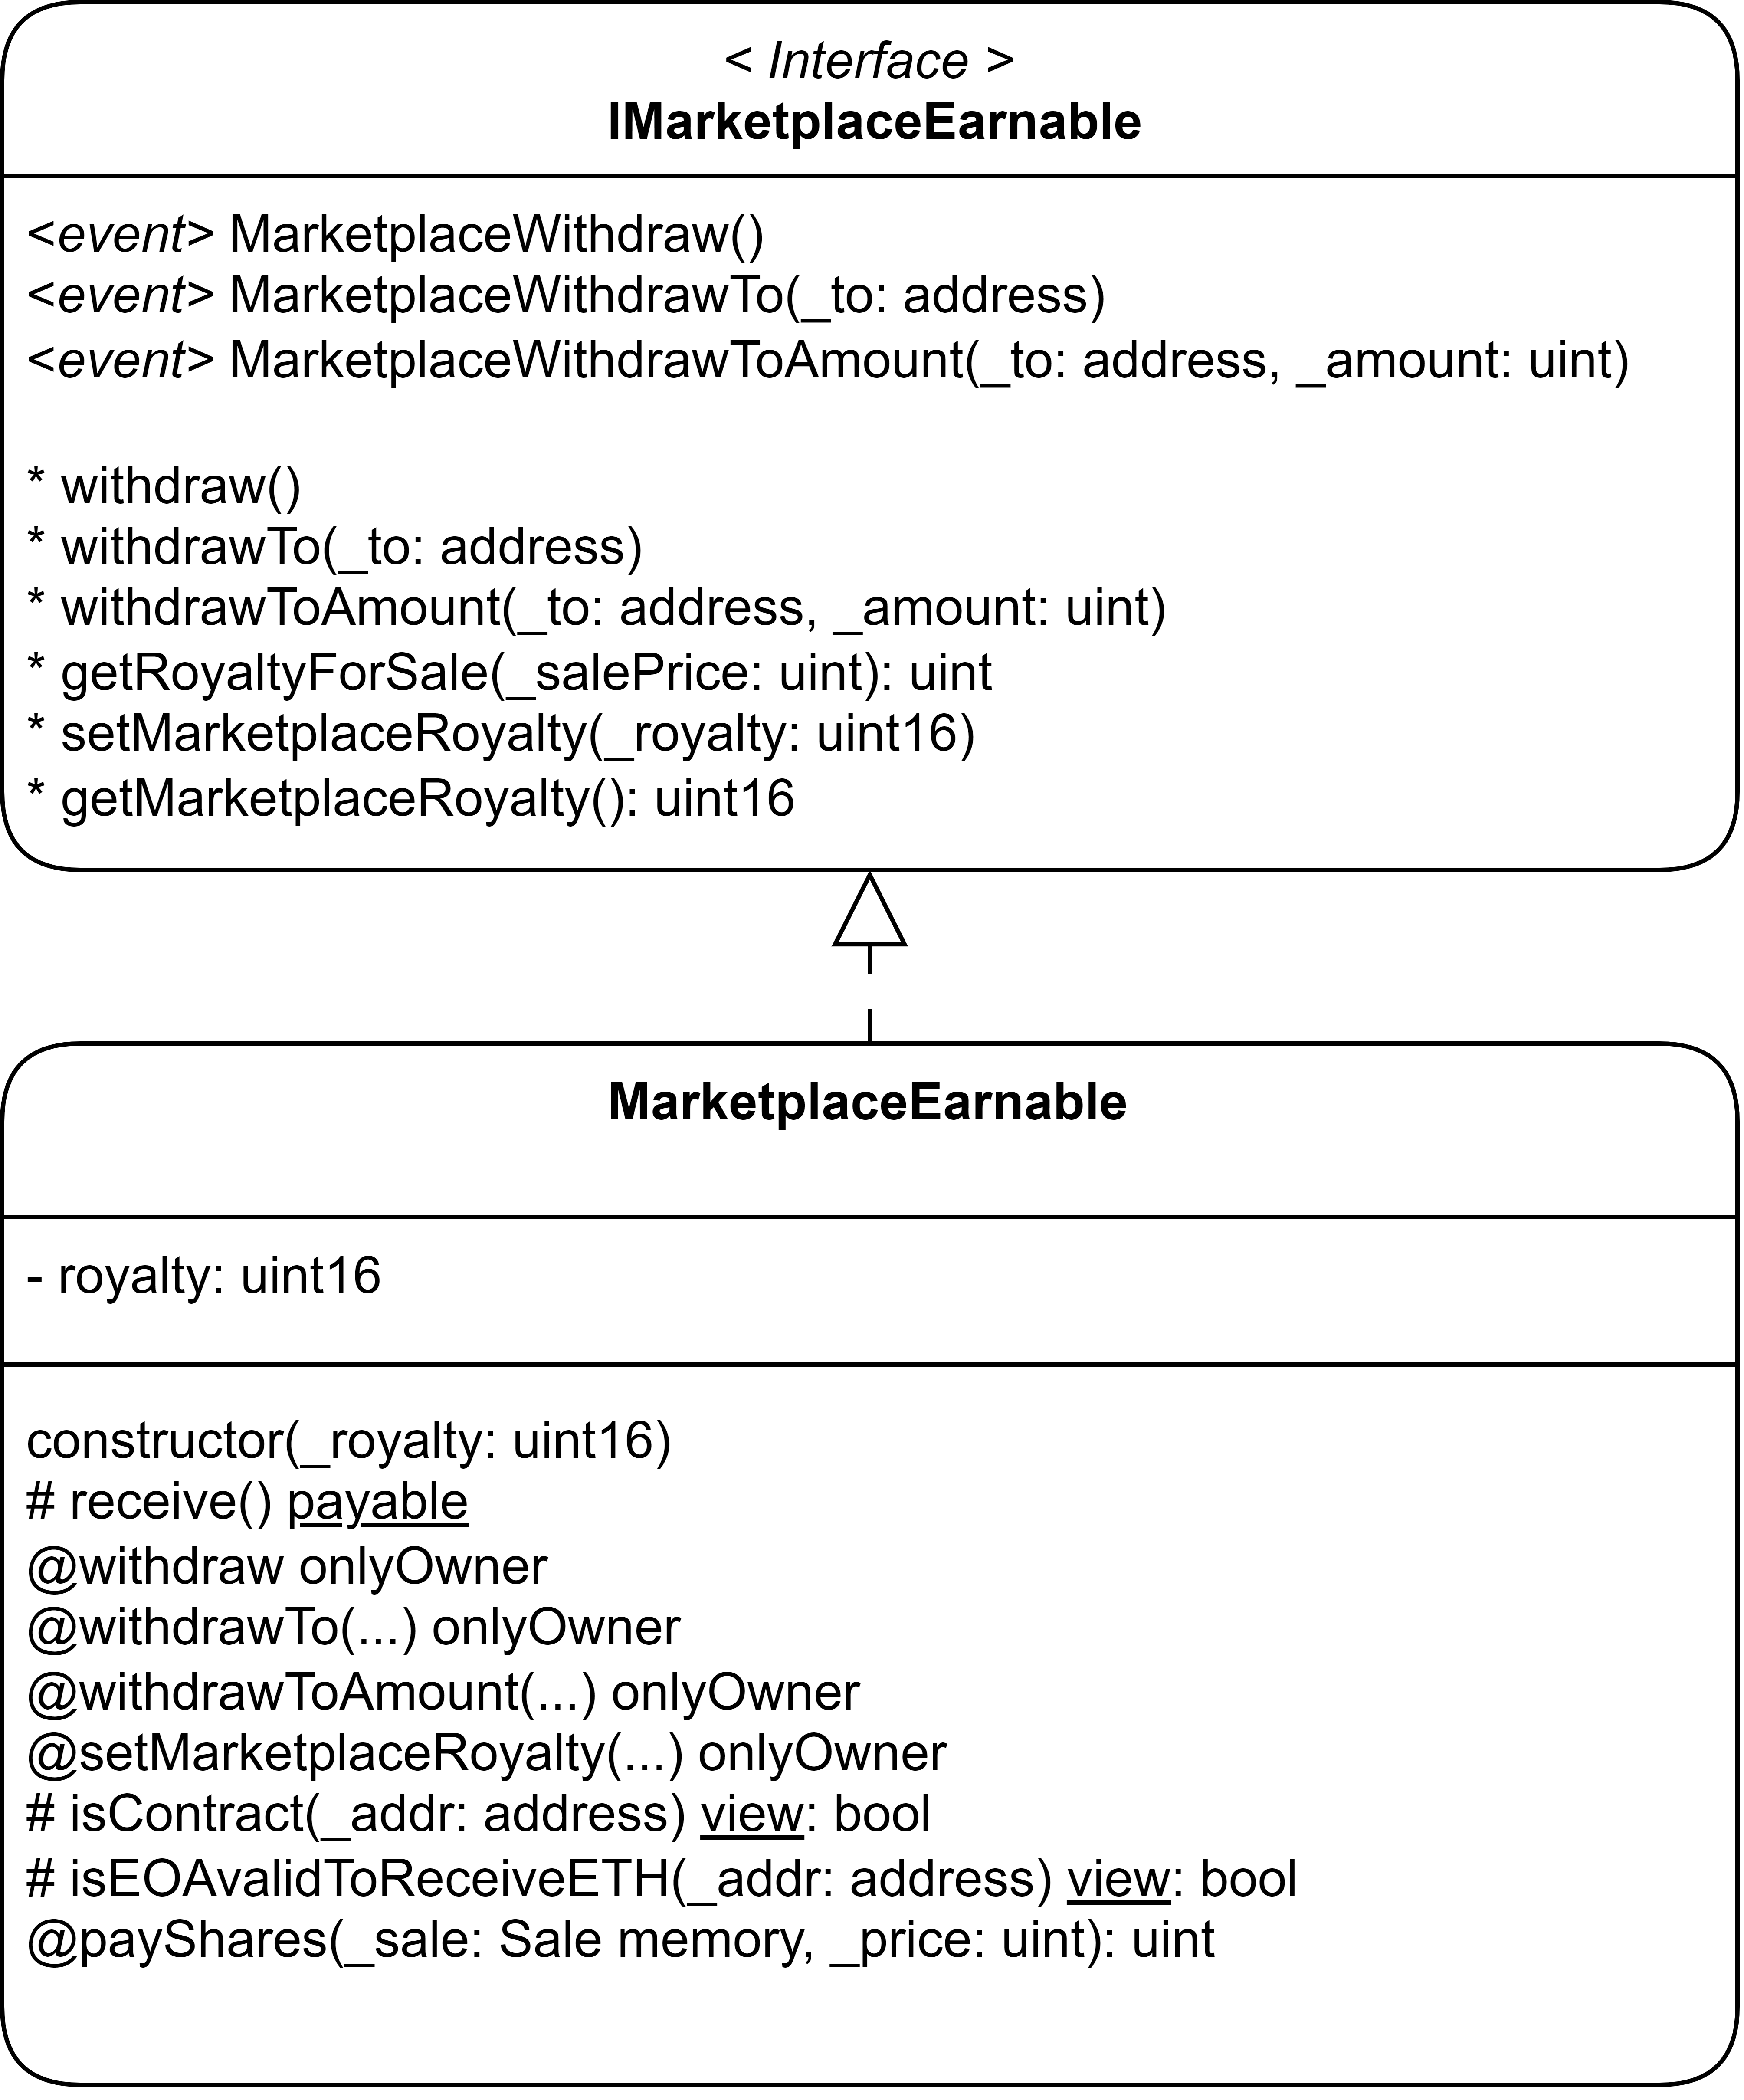
\includegraphics[width=0.7\textwidth]{images/blockchainContracts/MarketplaceEarnable.png}
    \caption{Marketplace Earnable}
    \label{fig:marketplaceEarnable}
\end{figure}

\paragraph{RoyaltyApplicable}
\label{sec:marketplace-royalty-applicable}

Il contratto \textit{RoyaltyApplicable} ha un funzionamento simile al contratto \hyperref[sec:marketplace-earnable]{\textit{Earnable}}. Ovvero, effettuando l'\textit{override} del metodo \textit{payShares} il saldo sarà diviso. In questo caso,
nel momento in cui avviene un acquisto il saldo inviato sarà separato tra il venditore e gli indirizzi definiti dal creatore dell'asset.

\begin{figure}[H]
    \centering
    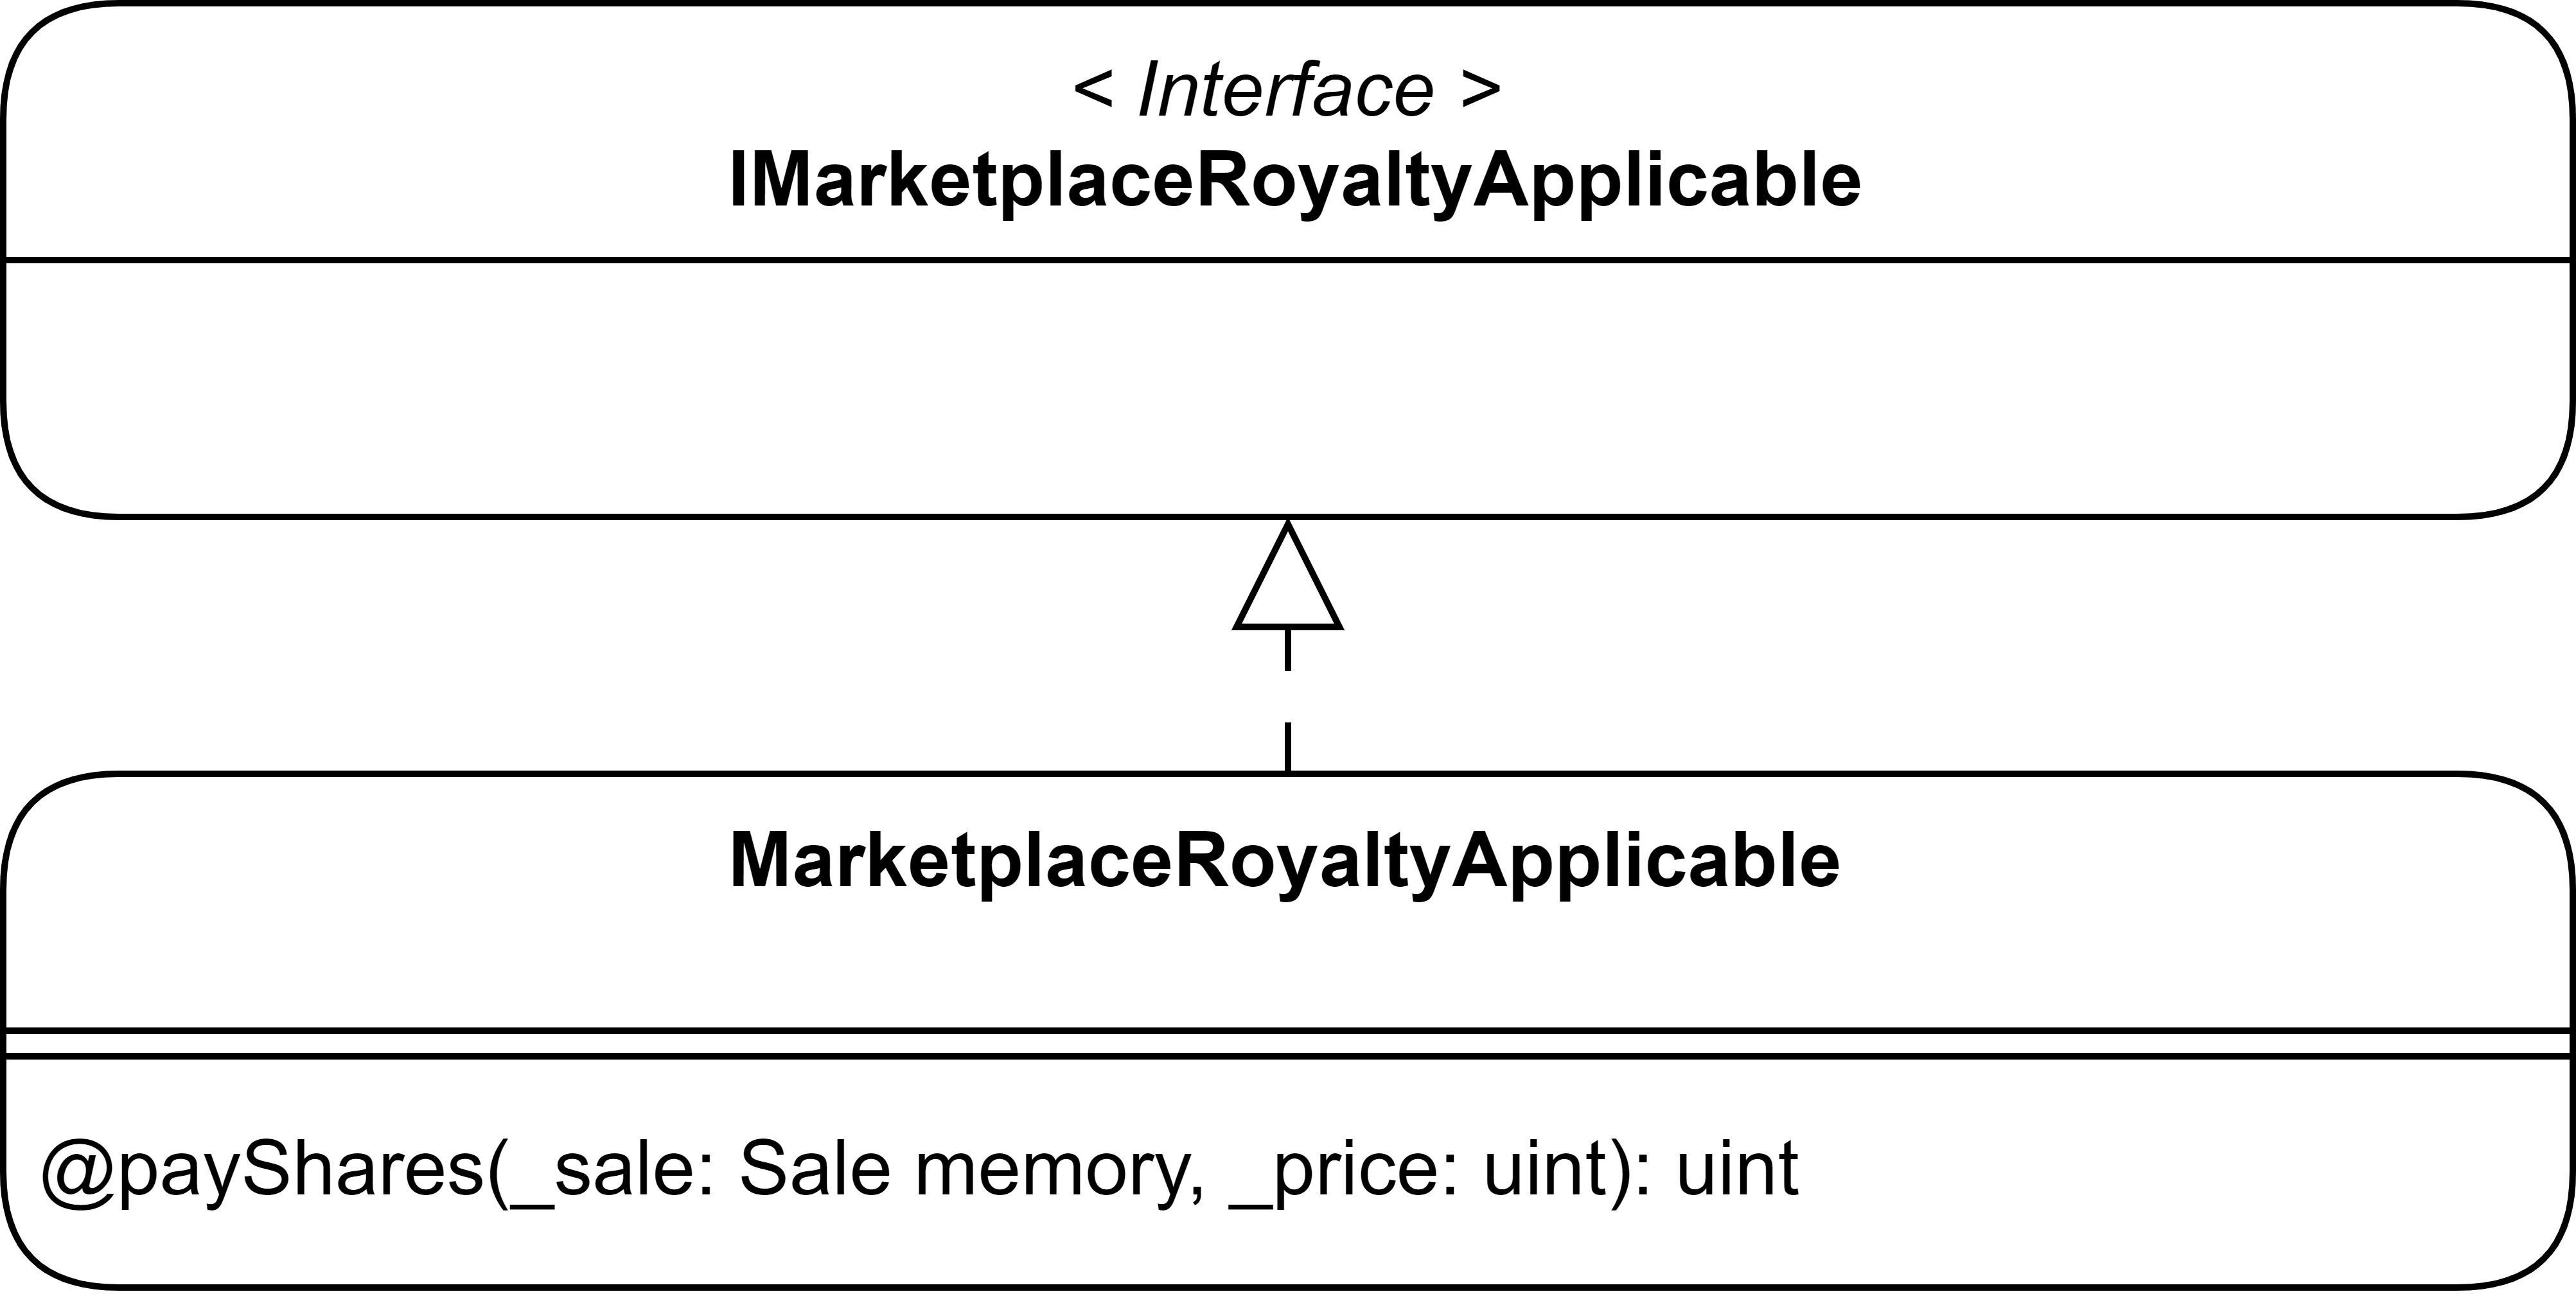
\includegraphics[width=0.7\textwidth]{images/blockchainContracts/MarketplaceRoyaltyApplicable.png}
    \caption{Marketplace RoyaltyApplicable}
    \label{fig:marketplaceRoyaltyApplicable}
\end{figure}


\paragraph{Cleanable}

All'interno del contratto \textit{Cleanable}, come rappresentato in figura \ref{fig:marketplaceCleanable}, sono presenti due metodi di gestione utilizzabili unicamente dall'amministratore, le loro funzionalità sono le seguenti:

\begin{itemize}
    \item \textit{cleanStorage}: Le informazioni relative a vendite cancellate o vendute rimangono all'interno del contratto. \textit{cleanStorage} permette di eliminare le informazioni relative a queste vendite allo scopo di ridurre la quantità di dati salvati all'interno del contratto, permettendo la riduzione dei tempi di attesa per l'esecuzione di alcune funzionalità sia \textit{on-chain} che \textit{off-chain}. Durante la progettazione del contratto è stato deciso di non cancellare queste informazioni all'acquisto, così da permettere agli utenti di risparmiare sulle \textit{gas fee}.
    \item \textit{cleanInqualities}: Questo metodo permette di eliminare le informazioni relative a vendite che non sono più corrette. Tale situazione può accadere nel momento in cui un utente trasferisce un asset in vendita esternamente al marketplace. In questo caso, la vendita rimarrebbe presente nel marketplace ma non sarebbe più valida. Un'alternativa per risolvere il problema è descritta nel capitolo \hyperref[sec:marketplace-royalty-applicable]{\textit{RoyaltyApplicable}}.
\end{itemize}

\begin{figure}[H]
    \centering
    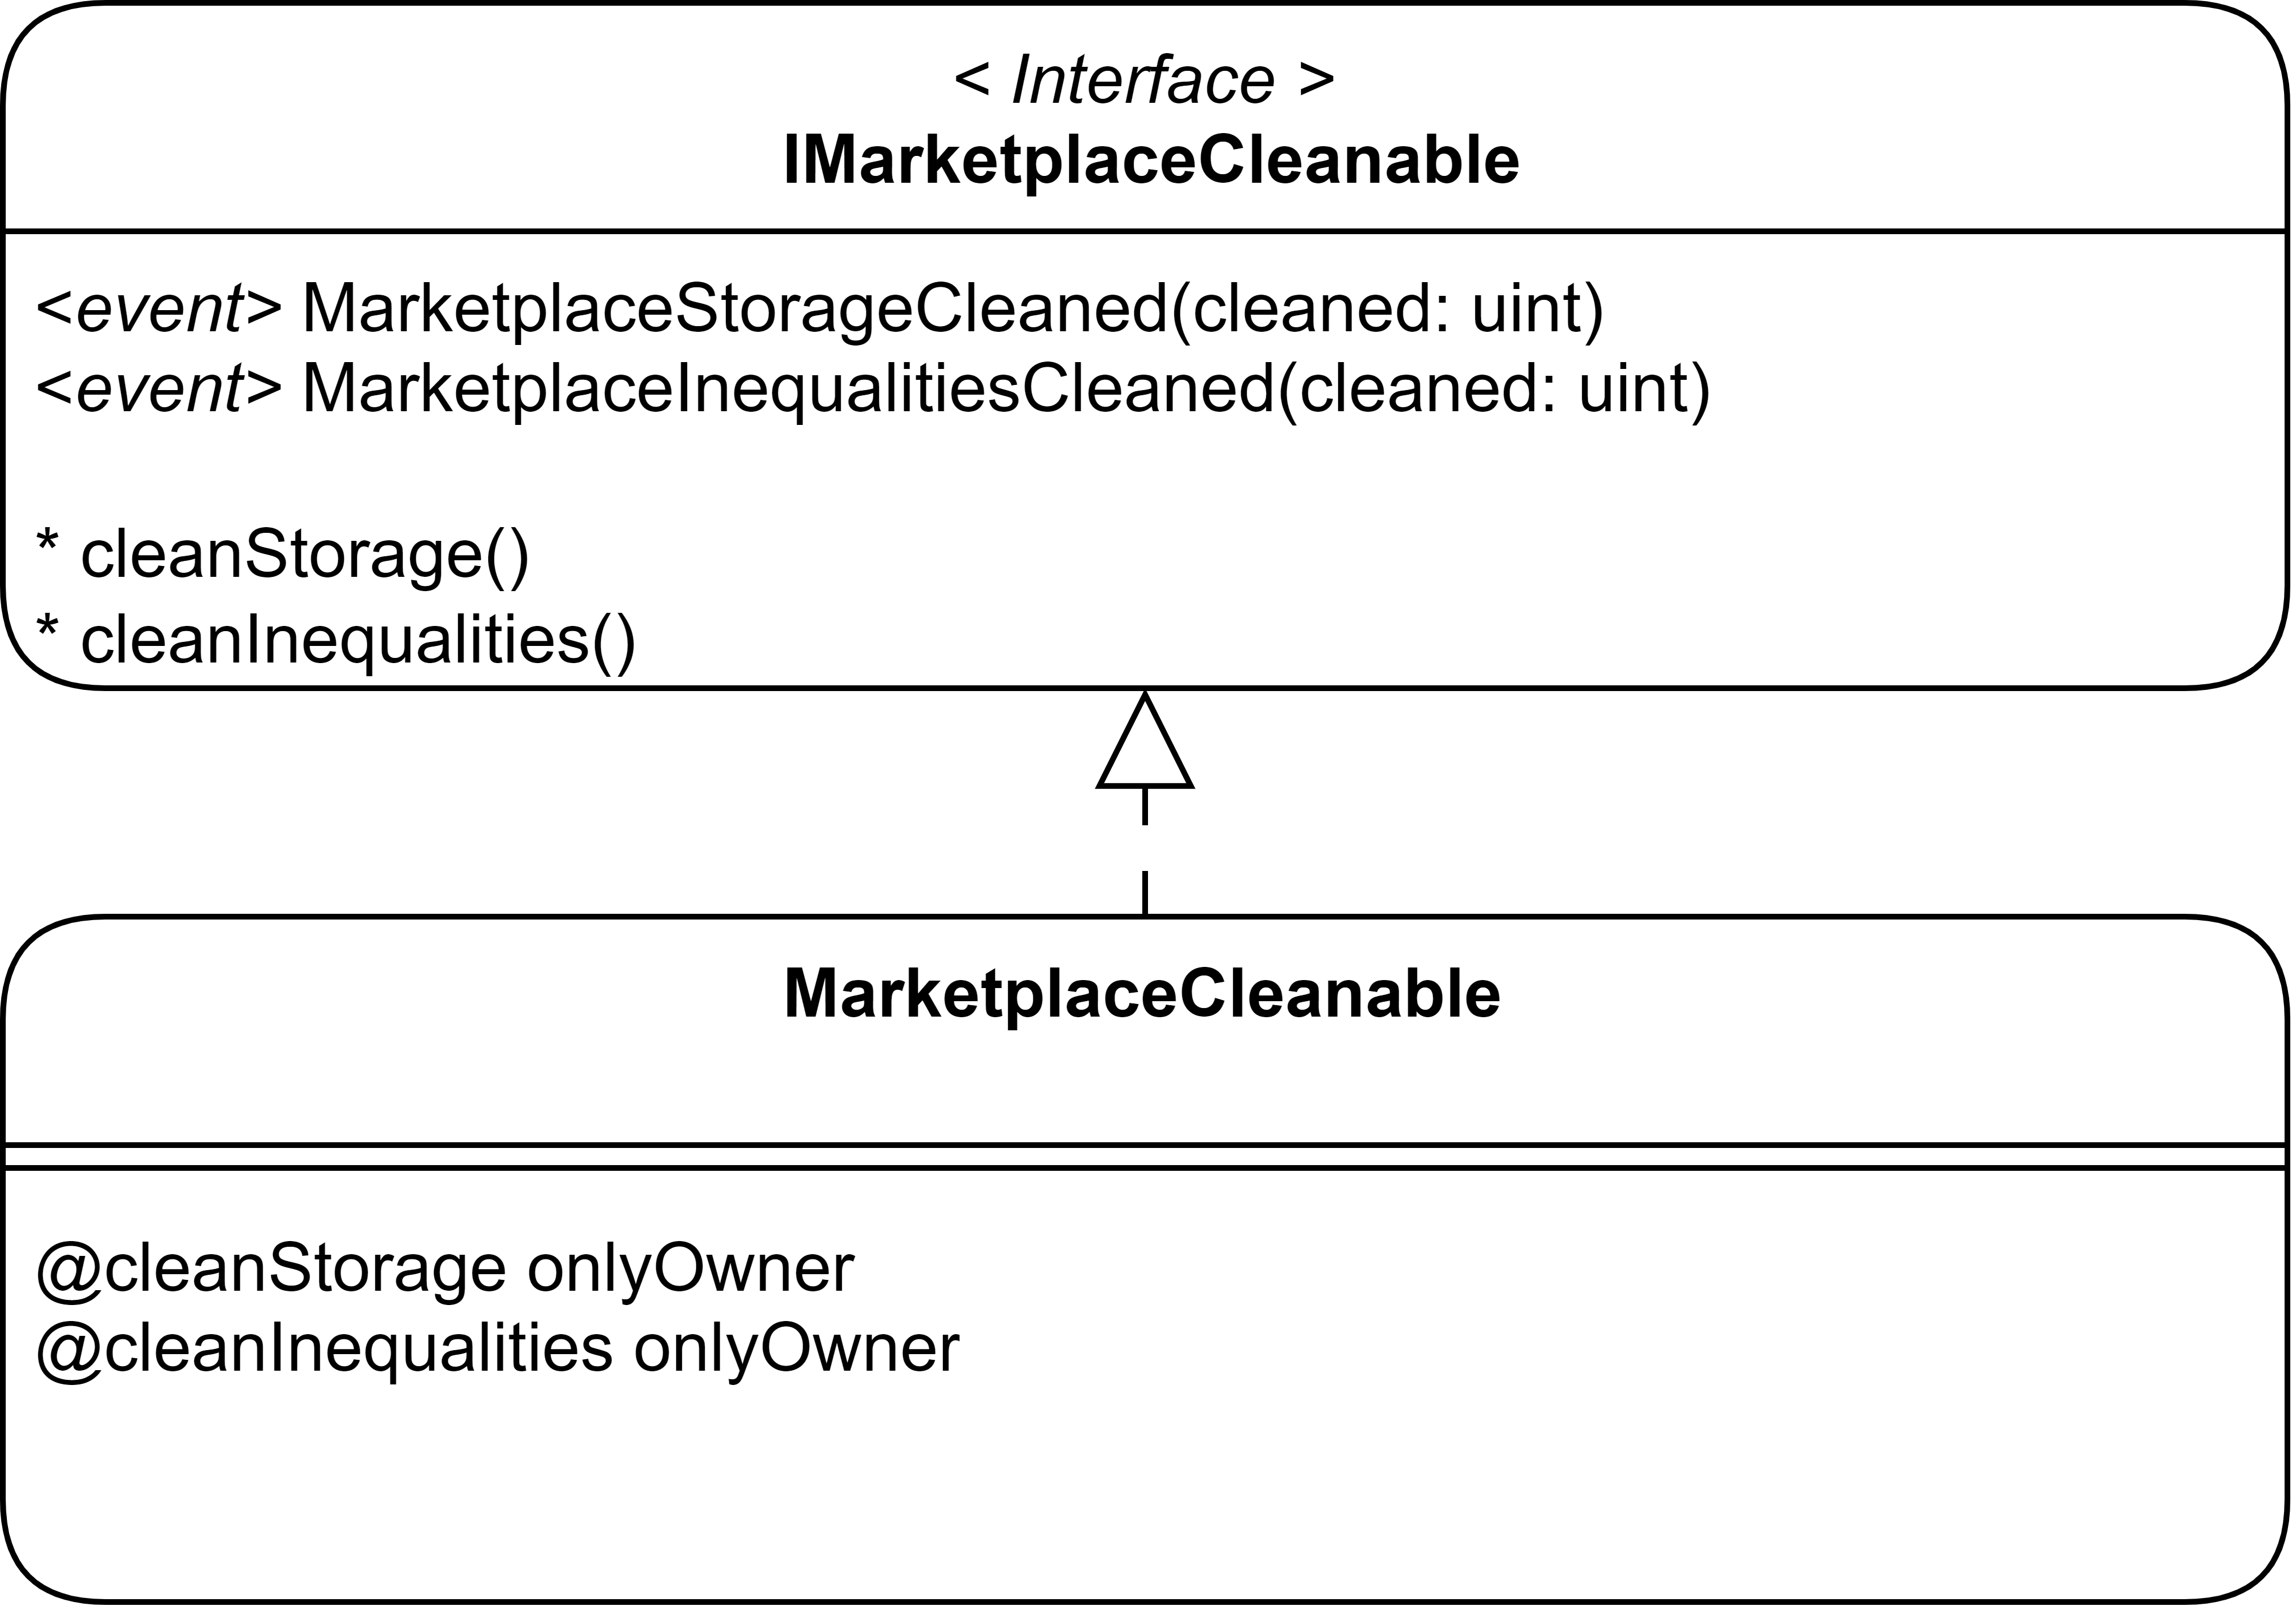
\includegraphics[width=0.7\textwidth]{images/blockchainContracts/MarketplaceCleanable.png}
    \caption{Marketplace Cleanable}
    \label{fig:marketplaceCleanable}
\end{figure}


\subsubsection{ERC721 Factory}

Come descritto nel capitolo \hyperref[sec:creazioneNFT]{\textit{Creazione NFT}}, l'utente ha tre possibilità per la generazione di un NFT, tra cui la creazione di una nuova collezione attraverso il \textit{depolyment} di un contratto ERC721. Per facilitare l'ultima operazione descritta, è stato sviluppato lo \textit{smart contract} \textit{ERC721 Factory}. Il quale permette di creare nuovi contratti utilizzando un \textit{template} chiamato \textit{Boilerplate ERC721}, analizzato nel prossimo capitolo. Come è possibile notare dalla figura \ref{fig:erc721Factory} il contratto presenta due metodi:

\begin{itemize}
    \item \textit{createERC721}: permette la creazione di un nuovo contratto ERC721, impostando un base URI per i metadati dei token (l'URI completo sarà composto da base URI + token ID), il nome e il simbolo della collezione. Inoltre, il metodo permette di impostare le \textit{royalties} di default per l'intero contratto e di effettuare l'operazione di \textit{mint} per un numero definito di asset.
    \item \textit{getAllERC721s}: questo metodo consente di ottenere tutti i contratti ERC721 creati attraverso la \textit{factory}. La sua utilità si presenta nel momento in cui l'utente vuole creare un nuovo NFT all'interno di una collezione già esistente. Infatti, filtrando in base all'\textit{owner} tutti i contratti ERC721, sarà possibile fornire all'utente unicamente quelli su cui ha il permesso di creare un nuovo NFT.
\end{itemize}

\begin{figure}[H]
    \centering
    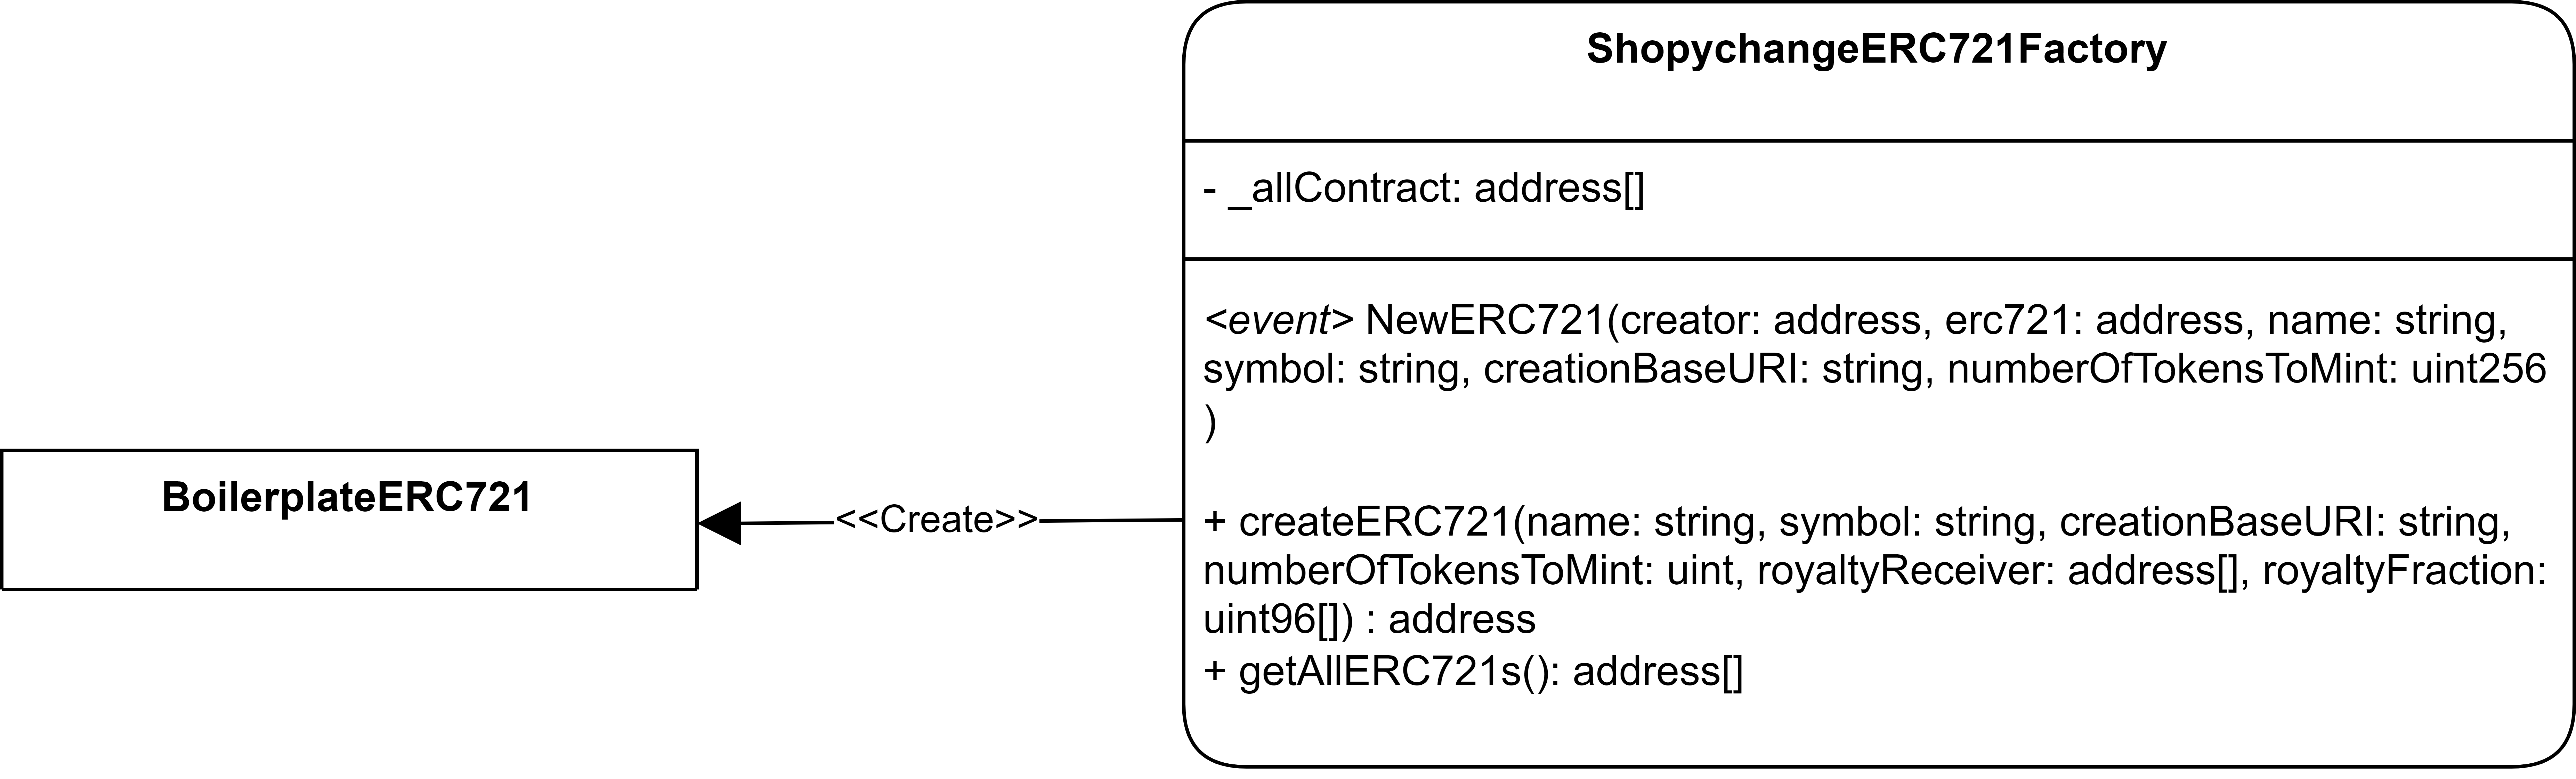
\includegraphics[width=0.7\textwidth]{images/blockchainContracts/ERC721Factory.png}
    \caption{ERC721 Factory}
    \label{fig:erc721Factory}
\end{figure}


\subsubsection{Boilerplate ERC721}

Il contratto \textit{Boilerplate ERC721} è un \textit{template} utilizzato per la creazione di nuovi contratti ERC721. Come visibile in figura \ref{fig:boilerplateERC721}, il contratto eredita da \textit{ERC721URIStorage}, \textit{ERC721Burnable} e \textit{ERC2981MultiReceiver}, questo permette di avere dei metadati per ogni token, di poter bruciare un token e di poter gestire le \textit{royalty} in maniera personalizzata.

\begin{figure}[H]
    \centering
    \includegraphics[width=0.7\textwidth]{images/blockchainContracts/BoilerplateERC721.png}
    \caption{BoilerplateERC721}
    \label{fig:boilerplateERC721}
\end{figure}

\paragraph{ERC2981MultiReceiver}
\label{sec:erc2981-multi-receiver}

Il contratto \textit{ERC2981MultiReceiver} è stato sviluppato per consentire la gestione delle \textit{royalty} in maniera personalizzata. 

Come visibile in figura \ref{fig:boilerplateERC721}, il contratto eredita da \textit{IERC2981Royalties}, il quale definisce le funzionalità obbligatorie per la gestione delle \textit{royalties}.

Come descritto più in dettaglio nel capitolo \hyperref[sec:utilizzo-erc2981-payment-splitter]{\textit{Utilizzo di ERC2981 e PaymentSplitter}} il contratto \textit{ERC2981MultiReceiver} è stato creato per poter gestire le \textit{royalties} con più di un ricevente. Infatti, già nel momento di creazione di un nuovo contratto \textit{BoilerplateERC721}, nel caso in cui vengano specificati più indirizzi, avverrà la creazione di un \textit{PaymentSplitter} di default. In questo modo, nel momento in cui avviene un acquisto, il saldo verrà diviso in base alla percentuale definita per ogni indirizzo. In aggiunta, il contratto permette la creazione di \textit{royalty} personalizzate per ogni token, creando contratti \textit{PaymentSplitter} all'occorenza.

\paragraph{PaymentSplitter}

Il contratto \textit{PaymentSplitter} offre la possibilità di dividere il saldo in base alla percentuale definita per ogni indirizzo. Nel momento in cui avviene un acquisto, il marketplace, o più specificamente il contratto \hyperref[sec:marketplace-royalty-applicable]{\textit{RoyaltyApplicable}}, invierà il saldo relativo alle \textit{royalties} al contratto \textit{PaymentSplitter}. Tuttavia, a causa di una limitazione implementativa del metodo \textit{receiver}, sarà compito dei riceventi di recupare il saldo ottenuto, l'operazione è possibile tramite il metodo \textit{release}. All'interno del capitolo \hyperref[sec:revenue-share]{\textit{Revenue Share}} è possibile osservare un esempio di utilizzo del contratto \textit{PaymentSplitter}.

\subsubsection{Storage}
Il contratto storage è semplicemente un contratto \textit{BoilerplateERC721} con la particolarità che chiunque può effettuare l'operazione di \textit{mint}. Esso è stato sviluppato per permettere a tutti glii utenti di creare un singolo asset senza la necessità di creare una collezione. 

\subsection{Scripts}

Per le operazioni di distribuzione dei contratti sono stati creati degli script appositi, i quali permettono l'automazione di alcuni processi ripetitivi.

Lo script chiamato \textit{copyArtifacts} permette di copiare gli artefatti generati dalla compilazione degli smart contracts in una cartella definita.

Lo script \textit{modifyEnv} ha lo scopo di modificare i file \textit{.env}, ovvero i file di configurazione presenti sia nel frontend che nel backend. Più in dettaglio, questo script permette di modificare il valore di variabili definite con uno nuovo. Il suo utilizzo è molto utile nel momento in cui si effettua il \textit{deploy} di un contratto. Infatti, il contratto appena distribuito avrà un indirizzo diverso rispetto a quello precedente ed è quindi necessario modificare i file di \textit{envirorment} per permettere al frontend e al backend di interagire con il nuovo contratto.

Infine, è stato creato uno script chiamato \textit{deployAll}, esso permette di distrubito tutti i contratti sopracitati aggiornando gli artefatti e modificando i file \textit{.env}.

\subsection{Test}

Per verificare il corretto funzionamento degli smart contracts sono stati sviluppati dei test utilizzando la libreria \textit{ethers}, già presente nel framework \textit{Hardhat}. I test effettuati sono di due tipi: \textit{unit test} e \textit{integration test}.
I primi si occupano di verificare il corretto funzionamento di una singola funzionalità all'interno di un contratto. Mentre i secondi, si occupano di verificare il corretto funzionamento di più funzionalità all'interno di più contratti oppure di un singolo contratto generato ereditando più moduli, come nel caso del contratto \textit{ShopychangeMarketplace}.

\subsection{Motivazioni e Alternative}

La scelta che ha portato all'utilizzo di \textit{Hardhat} è stata fatta in quanto è un framework molto utilizzato e ben documentato, inoltre permette di creare un'istanza di un nodo locale, così da poter utilizzare una blockchain locale rendendo più semplice lo sviluppo e i test dell'intera applicazione. Per quanto riguarda la scelta del linguaggio di programmazione, è stato deciso di utilizzare \textit{Solidity} in quanto è il linguaggio più utilizzato per lo sviluppo di smart contracts. Inoltre, è possibile trovare una vasta documentazione e numerosi esempi di codice. 

In aggiunta, Durante lo svolgimento del progetto è stato utilizzato anche il webtool \textit{Remix}, il quale permette di scrivere, compilare e distribuire gli \textit{smart contracts}. In aggiunta, \textit{Remix} ha la funzionalità di poter interagire con gli \textit{smart contracts} attraverso dei semplici pulsanti, velocizzando l'interazione.

Inoltre, durante la fase di sviluppo è stato deciso di non utilizzare \textit{Typechain}, il quale permette di generare dei tipi TypeScript a partire dagli smart contracts. Questa scelta è stata fatta in quanto la libreria di interazione con i contratti a livello frontend (\textit{wagmi}) non supporta i tipi generati da \textit{Typechain}. Tuttavia, è possibile utilizzare \textit{Typechain} in combinazione con \textit{ethers} (una libreria largamente utilizzata per l'interazione con gli smart contracts).

Le alternative in ambito implementativo sono molteplici, così come le tecnologie utilizzabili. In particolare, per lo sviluppo degli smart contracts è possibile utilizzare diversi linguaggi di programmazione, tra cui \textit{Solidity}, \textit{Vyper} e \textit{Fe}. Anche i framework utilizzabili sono numerosi, tra cui \textit{Hardhat}, \textit{Truffle}\footnote{https://trufflesuite.com/} e \textit{Embark}\footnote{https://framework.embarklabs.io/}.

\chapter{Approccio al problema}
\label{sec:approccioProblema}

Nel seguente capitolo verranno analizzati i requisiti del sistema, le scelte tecnologiche e implementative, nonché la metodologia di sviluppo adottata. 

Per affrontare il \hyperref[sec:problema]{problema} sono stati analizzati i principali \textit{marketplace decentralizzati} esistenti, in particolare \textit{OpenSea}\footnote{https://opensea.io/} e \textit{Rarible}\footnote{https://rarible.com/}, per comprendere le principali funzionalità e caratteristiche che un \textit{marketplace} dovrebbe avere.

Più in dettaglio, sono stati analizzati i seguenti aspetti:
\begin{itemize}
    \item Facilità d'uso
    \item Funzionalità disponibili
    \begin{itemize}
        \item Creazione di un asset
        \item Acquisto di un asset
        \item Vendita di un asset
        \item Modifica o cancellazione della vendita di un asset
    \end{itemize}
    \item Revenue share
    \item Interoperabilità con altri marketplace
    \item Conformità all'ideologia di decentralizzazione
    \item Recupero dei dati dalla blockchain
\end{itemize}

Come concordato con il relatore, è stato deciso di creare un marketplace che rispetti al meglio i principi di decentralizzazione, così da essere il più possibile trasparente. 

La scelta delle tecnologie utilizzate è stata fatta dallo studente, con l'approvazione del relatore, in modo da poter acquisire nuove conoscenze e competenze in ambito di sviluppo di applicazioni web (backend e frontend), di smart contracts e blockchain.

Il progetto realizzato è una \textit{Decentralized Appllication} (dApp), ovvero un'applicazione che utilizza la blockchain per fornire funzionalità e servizi. In contrasto alle applicazioni tradizionali che operano su server centralizzati, le dApp operano su una rete decentralizzata, consentendo miglioramenti come maggiore sicurezza dei dati, resistenza alla censura e trasparenza nelle operazioni. \cite{bitpanda-dApp}

La \textit{Decentralized Appllication} realizzata è composta da diversi componenti, ognuna delle quali è stata sviluppata utilizzando tecnologie e linguaggi di programmazione differenti, in particolare la soluzione realizzata è composta da:

\begin{itemize}
    \item \textit{Backend}: Si occupa della gestione delle richieste provenienti dal frontend, in particolare del recupero dei dati presenti nella blockchain e nel database, nonché della loro elaborazione e restituzione al frontend.
    \item \textit{Frontend}: Si occupa di gestire l'interazione con l'utente, richiedendo i dati al backend e mostrandoli all'utente, inoltre si occupa di gestire le richieste di interazione con la blockchain.
    \item \textit{Blockchain / Smart contracts}: \textit{Core} del progetto, più smart contracts si occupano di gestire la logica di \textit{business}, in particolare la creazione, modifica e vendita di un asset, nonché la gestione del revenue share.
    \item \textit{Database}: All'interno del database vengono salvati unicamente alcuni dati di personalizzazione utente del marketplace.
\end{itemize}

\section{Requisiti}

Analizzando i requisiti del sistema, si è deciso di suddividerli in due categorie: requisiti funzionali e requisiti non funzionali. Essi permettono di definire le funzionalità che il sistema deve possedere e le sue caratteristiche. 

\subsection{Requisiti funzionali}

I requisiti funzionali forniscono una chiara descrizione delle funzionalità e ciò che gli utenti si aspettano dal sistema.
Di seguito sono elencati i requisiti funzionali del sistema: 
\begin{itemize}
    \item \textit{RF1}: L'utente ha la possibilità di creare un asset
    \item \textit{RF2}: L'utente ha la possibilità di vendere un asset
    \item \textit{RF3}: L'utente ha la possibilità di acquistare un asset
    \item \textit{RF4}: L'utente ha la possibilità di visualizzare gli asset in vendita
    \item \textit{RF5}: L'utente ha la possibilità di modificare o cancellare un asset in vendita
    \item \textit{RF6}: La gestione della piattaforma è basata su un sistema a ruoli e permessi
    \item \textit{RF7}: Un asset può essere posseduto da un solo utente, ma altri utenti possono avere ruoli gestionali su di esso
    \item \textit{RF8}: Il sistema deve essere in grado di gestire aspetti di mercato come il \textit{listing} e \textit{revenue share}
\end{itemize}

\subsection{Requisiti non funzionali}

I requisiti non funzionali definiscono i limiti e vincoli nei quali il sistema deve operare.
Di seguito sono elencati i requisiti non funzionali del sistema:
\begin{itemize}
    \item \textit{RNF1 (Prestazioni)}: Il sistema deve essere in grado di elaborare le transazioni in modo rapido ed efficiente
    \item \textit{RNF2 (Sicurezza)}: Il sistema deve essere progettato per essere sicuro e trasparente, sia per venditori che per acquirenti
    \item \textit{RNF3 (Usabilità)}: Il sistema deve essere progettato per essere semplice ed intuitivo
    \item \textit{RNF4 (Scalabilità)}: Il sistema deve poter gestire un numero elevato di utenti e transazioni
    \item \textit{RNF5 (Integrità)}:  Il sistema deve essere in grado di fornire dati sempre aggiornati e veritieri
\end{itemize}

\newpage

\section{Creazione NFT}
\label{sec:creazioneNFT}
Come precedentemente descritto nei capitoli \hyperref[sec:erc721]{\textit{ERC721}} e \hyperref[sec:erc1155]{\textit{ERC1155}}, ovvero gli standard utilizzati per la creazione di NFT, alcuni dati relativi all'asset sono salvati all'interno dello \textit{smart contract}. Di norma i dati salvati sono:
\begin{itemize}
    \item \textit{Token ID}: Identificativo univoco dell'asset
    \item \textit{Token Owner}: Indirizzo Ethereum del possessore dell'asset
    \item \textit{Collection name}: Nome della collezione
    \item \textit{Collection symbol}: Simbolo della collezione, solitamente composto da 3 lettere
    \item \textit{Token URI}: URL che punta ad un file JSON contenente le informazioni relative all'asset
\end{itemize}

Come si può notare, i dati salvati nello \textit{smart contract} sono pochi e non contengono informazioni riguardanti l'asset stesso. Questo perché, le informazioni riguardanti l'asset, ovvero i \textit{metadati}, sono salvati in un file JSON esterno. Questo file è accessibile tramite l'URL definito come \textit{Token URI}, esso può essere diverso per ogni asset oppure avere una base comune e differenziarsi attraverso il \textit{Token ID}.

Per compatibilità con l'idea di decentralizzazione, il file JSON contenente i metadati dell'asset è spesso salvato su una rete peer-to-peer, come ad esempio \hyperref[sec:ipfs]{\textit{IPFS}}. Questo permette di avere un file accessibile da chiunque e immutabile, senza la necessità di un server centralizzato.



Come sarà possibile vedere a livello grafico nel capitolo \hyperref[sec:creazione]{\textit{Frontend - creazione}}, è stato deciso di fornire tre opzioni per la creazione di un NFT:

\begin{itemize}
    \item \textit{Creazione di una collezione}: Permette di creare una collezione di NFT, ovvero uno \textit{smart contract} che implementa lo standard ERC721.
    \item \textit{Creazione di un NFT su una propria collezione}: Permette di creare un NFT all'interno di una collezione precedentemente creata. 
    \item \textit{Aggiunta di un NFT ad una collezione comune}: Permette di aggiungere un NFT ad una collezione comune, ovvero ad uno \textit{smart contract} già esistente. Questo permette di ridurre notevolmente i costi di creazione.
\end{itemize}

Come è possibile osservare in figura \ref{fig:creazioneNFT}, il processo di creazione di un NFT completo consiste inizialmente nel creare un file JSON contenente i metadati dell'asset e salvarlo su una rete peer-to-peer. Il prossimo passo consiste nel creare uno \textit{smart contract} (oppure aggiungere il token ad uno \textit{smart contract} già esistente) che implementi uno degli standard precedentemente descritti e che sia collegato all'URL del file JSON creato. Infine, è necessario pubblicare lo \textit{smart contract} sulla rete Ethereum.

\begin{figure}[H]
    \centering
    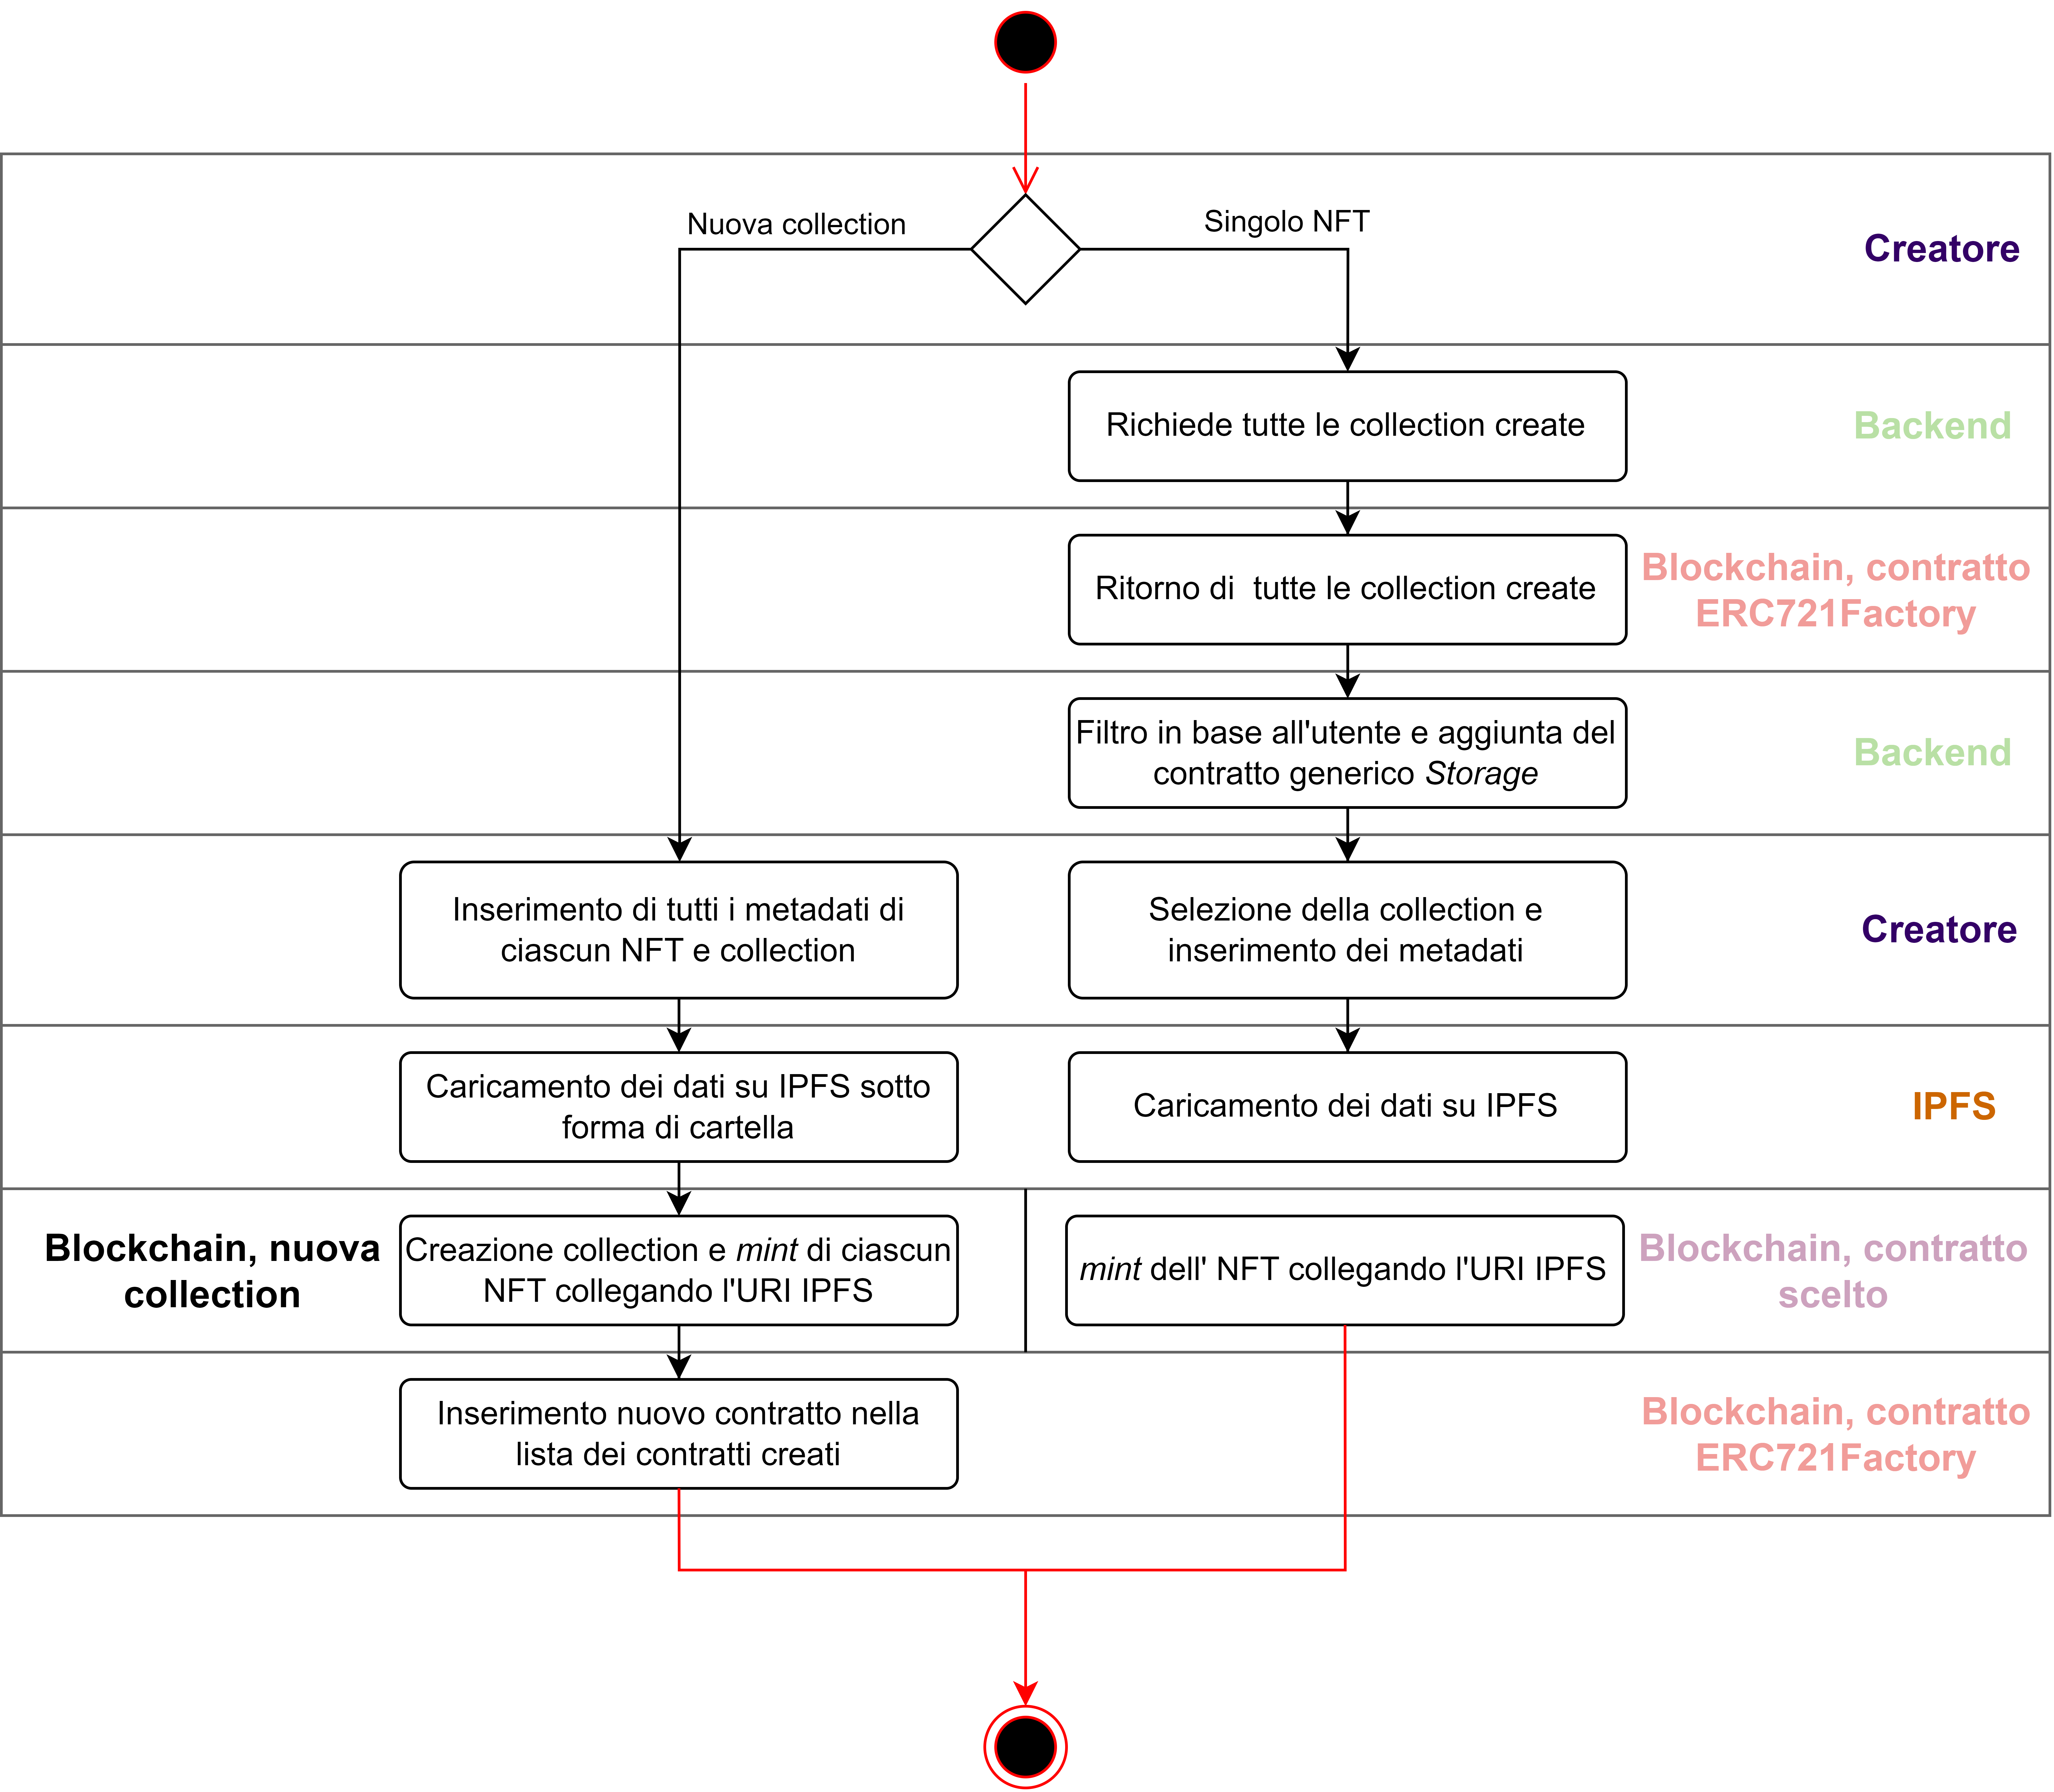
\includegraphics[width=1\textwidth]{images/creazioneNFT.png}
    \caption{Schema del processo di creazione di un NFT o più}
    \label{fig:creazioneNFT}
\end{figure}

\section{Recupero dei dati dalla blockchain}
\label{sec:recuperoDatiBlockchain}

Le blockchain possono contenere una grande quantità di dati e spesso per recuperare le informazioni di interesse è necessario analizzare l'intera blockchain filtrando le varie transazioni. Per esempio, l'operazione necessaria per recuperare tutti gli NFT presenti in una collezione, consiste nell'analizzare tutti gli eventi di \textit{transfer} emessi e selezionare unicamente quelli destinati ad un indirizzo specifico che non sia lo \textit{zero address}, ovvero l'indirizzo che rappresenta l'assenza di un indirizzo valido.

Come è possibile dedurre, questa semplice operazione può portare ad avere tempi di attesa più lunghi rispetto a quelli di un database tradizionale. 

Per semplicità, all'inizio del progetto è stato scelto di utilizzare un servizio di terze parti per recuperare i dati dalla blockchain. Si è optato per  \textit{Alchemy}\footnote{https://www.alchemy.com/}, il quale tramite alcune API permette di recuperare facilmente i dati necessari. Poichè implementano un sistema di \textit{caching}, i tempi di risposta sono molto più veloci rispetto a quelli che si avrebbero interrogando direttamente la blockchain.

Considerato che, il servizio da loro offerto risulta gratuito fino ad un certo numero di richieste, è stato deciso di utilizzare questo servizio unicamente nella fase iniziale. Inoltre, il servizio presenta alcune limitazioni e incongruenze sui dati. Per esempio, anche se un NFT è stato \textit{burned}, ovvero distrutto, il servizio continua a restituire l'informazione che l'NFT è ancora presente nella collezione.

Perciò, per avere un controllo maggiore sui dati, è stato implementato un sistema di recupero dati che non dipendesse da servizi esterni. Come verrà analizzato più in dettaglio nel capitolo \hyperref[sec:backend]{\textit{Backend}}, sono state implementate delle API che permettono di recuperare i dati direttamente dalla blockchain. Per fare ciò, è stato necessario imporre una limitazione sui dati che è possibile recuperare. In particolare, è possibile recuperare i dati di una collezione solamente se si conosce l'indirizzo del contratto che la rappresenta. Infatti, all'interno del interfaccia grafica è possibile gestire gli indirizzi delle collezioni che si vogliono monitorare. 


\section{Revenue Share}
\label{sec:revenue-share}
Nel seguente capitolo verrà analizzato il concetto di \textit{revenue share}, le soluzioni implementate nei principali marketplace e i problemi che ne derivano. In aggiunta, verranno analizzate le soluzioni proposte dallo studente.

Il \textit{revenue share} è un aspetto fondamentale di un marketplace, esso permette di distribuire i guadagni (\textit{royalty}) tra i vari operatori, i quali possono essere il creatore dell'asset, il marketplace stesso e/o eventuali altri utenti definiti dal creatore.

La gestione del \textit{revenue share} è stata implementata tramite smart contracts, in modo da garantire trasparenza e sicurezza. 
Essendoci più attori coinvolti, il \textit{revenue share} è stato diviso in due parti:

\begin{itemize}
    \item Marketplace \textit{revenue share}
    \item Creator / Users \textit{revenue share}
\end{itemize}

Come si può osservare in figura \ref{fig:distribuzione-royalty} l'ordine di detrazione del \textit{revenue share} consiste nel sottrarre prima il \textit{revenue share} del marketplace e poi quello del creatore. 

\begin{figure}[H]
    \centering
    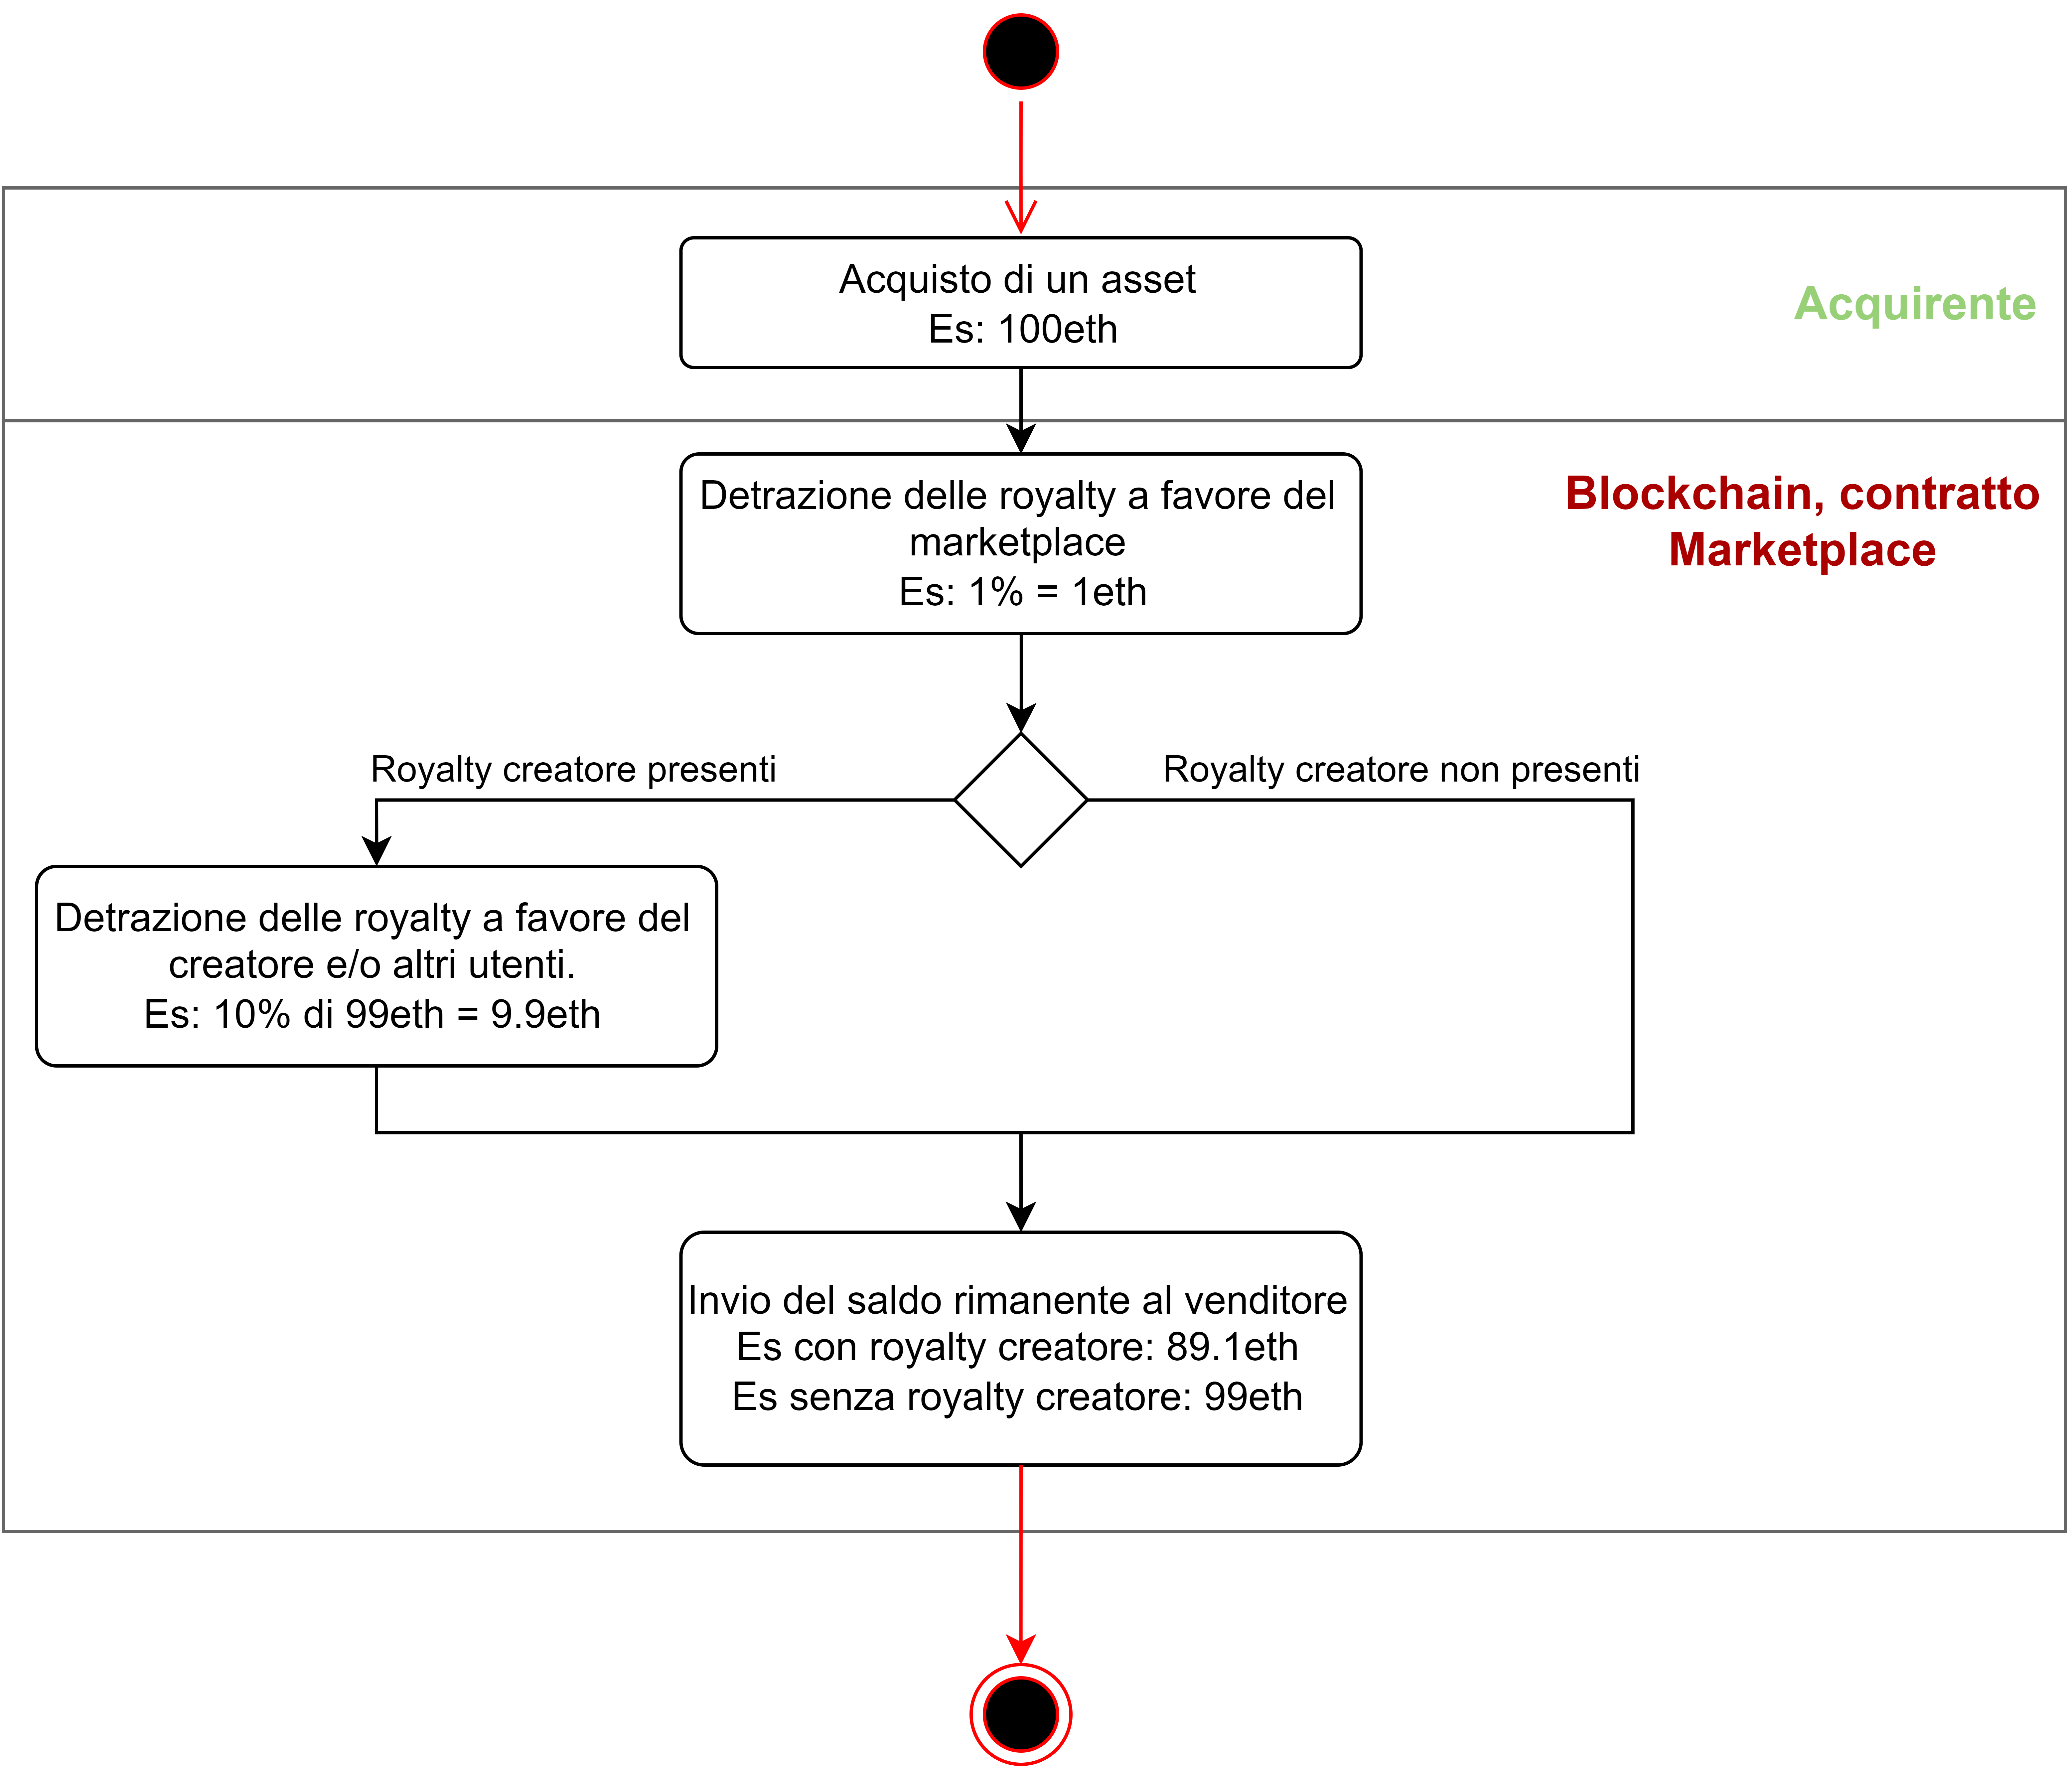
\includegraphics[width=0.8\textwidth]{images/SuddivisioneRoyalty.png}
    \caption{Suddivisione del revenue share}
    \label{fig:distribuzione-royalty}
\end{figure}



\subsection{Marketplace revenue share}
Come sarà approfondito nel capitolo \hyperref[sec:smart-contract-shopychange]{\textit{Blockchain - Smart contracts}}, il contratto principale del marketplace è composto da più moduli che si occupano di gestire le varie funzionalità di esso.

In particolare, il modulo \textit{MarketplaceEarnable} si occupa di gestire il \textit{revenue share} del marketplace, le sue funzionalità sono:

\begin{itemize}
    \item Salvare la percentuale di \textit{revenue share} a favore del marketplace.
    \item Fornire metodi di lettura e scrittura della percentuale di \textit{revenue share}, nonchè del calcolo del \textit{revenue share} in base al prezzo di vendita di un asset.
    \item Fornire metodi di ritiro dell'ammontare ottenuto dalle varie vendite.
\end{itemize}

Tramite queste funzionalità l'utente amministratore ha la possibilità di modificare e ritirare il \textit{revenue share} in qualsiasi momento. Per semplicità, è stata sviluppata un'interfaccia grafica che permette l'interazione con lo \textit{smart contract}, analizzata più in dettaglio nel capitolo \hyperref[sec:admin-dashboard]{\textit{Admin Dashboard}}.

\subsection{Creator / Users revenue share}
La ripartizione del \textit{revenue share} a favore del creatore risulta più complessa, essendo un tema attualmente in fase di sviluppo con diverse soluzioni proposte.

Il problema nasce dal fatto che non esiste uno standard ad oggi largamente utilizzato, il che ha portato i marketplace a sviluppare soluzioni proprietarie e non interoperabili tra loro. 

La causa principale di questa mancanza è a livello implementativo, non è possibile sapere se l'asset è stato acquistato tramite un marketplace o se il possessore abbia deciso di cederlo, dove in quest'ultimo caso il \textit{revenue share} non dovrebbe essere applicato.
Più in dettaglio, nel momento in cui avviene la chiamata ai diversi metodi di \textit{transfer}, definiti negli standard \textit{ERC721} e \textit{ERC1155}, il valore inviato con la transazione (ovvero il prezzo di vendita) non è accessibile, in quanto i metodi di \textit{transfer} sono di tipo \textit{non payable}, ovvero non permettono di inviare ETH. 

Perciò, per risolvere questo problema sono state analizzate le soluzioni implementate da due dei marketplace più famosi e utilizzati, cioè \textit{OpenSea}\footnote{https://opensea.io/} e \textit{Rarible}\footnote{https://rarible.com/}.

\begin{itemize}
    \item \textit{OpenSea} \cite{operator-filter-registry}: la soluzione da loro adottata si basa su smart contracts.
    In particolare, su un registro distribuito chiamato \textit{Operator Filter Registry} che permette di definire una lista di indirizzi abilitati alla gestione degli \textit{assets}. 

    Il creatore di una collezione dovrà modificare il proprio contratto  \textit{ERC721} o \textit{ERC1155} per risultare compatibile. Tramite questa modifica il nuovo contratto delegherà il controllo degli operatori approvati all'\textit{Operator Filter Registry}.

    L'\textit{enforcement}, ovvero il controllo che le \textit{revenue share} siano ripartite nel modo definito, avviene semplicemente con il fatto che, i marketplace riconosciuti per \textbf{non} applicare il \textit{revenue share} vengono inseriti in una \textit{blacklist} e quindi non possono gestire gli \textit{assets}.

    Il registro distribuito, inizialmente gestito e popolato da OpenSea, è ora gestito dal gruppo \textit{Creator Ownership Research Institute} (CORI).

    In aggiunta, i marketplace che sono riconosciuti per applicare il \textit{revenue share} hanno la possibilità di implementare il sistema di \textit{revenue share} a loro piacimento.
    \item \textit{Rarible} \cite{rarible-community-marketplaces}: la soluzione implementata da Rarible consiste anch'essa in un registro distribuito tra una lista di marketplace creati con l'aiuto di Rarible stesso, questo gruppo è chiamato \textit{Community Marketplaces}.
\end{itemize}

Le soluzioni implementate da OpenSea e Rarible sono molto simili, tuttavia presentano problemi di interoperabilità. Nel momento in cui un creatore decidesse di utilizzare uno dei due marketplace, dovrebbe ripetere la stessa configurazione nell'altro mercato digitale. Inoltre, potrebbe essere necessario modificare anche lo \textit{smart contract} così da risultare compatibile, il che potrebbe essere un problema per i creatori meno esperti. Purtroppo però, anche con gli accorgimenti sopra descritti, non è possibile garantire che il \textit{revenue share} venga applicato correttamente in altri marketplace.

Riassumendo, la gestione di \textit{revenue share} presenta due principali problematiche:
\begin{enumerate}
    \item \textit{Interoperabilità}: Non esiste uno standard largamente utilizzato e quindi non è possibile garantire l'interoperabilità tra i diversi marketplace
    \item \textit{Enforcement}: Non è possibile essere sicuri che il \textit{revenue share} venga applicato correttamente, essendo un'azione che deve essere effettuata in modo volontario dal marketplace 
\end{enumerate}

I due problemi sopra descritti hanno soluzioni non compatibili tra loro. Analizzando più in dettaglio le soluzioni proposte da OpenSea e Rarible, è possibile notare che entrambe presentano un registro distribuito che permette di definire una lista di marketplace abilitati alla gestione degli \textit{assets}, tuttavia risulta essere un gruppo chiuso, non rispecchiando l'ideologia di decentralizzazione. D'altronde, in caso di gruppo aperto ed essendo il pagamento di \textit{revenue share} un'azione volontaria, non è possibile garantire che il \textit{revenue share} venga applicato correttamente.

Nei prossimi capitoli verranno analizzate in maniera più approfondita le soluzioni proposte.

\subsubsection{Utilizzo di ERC2981 e PaymentSplitter}
\label{sec:utilizzo-erc2981-payment-splitter}

La prima soluzione implementata nel marketplace \textit{Shopychange}, include l'utilizzo di una variante dello standard ERC2981. Come descritto nel capitolo \hyperref[sec:erc2981]{\textit{ERC2981}}, questo standard permette di aggiungere le informazioni relative al \textit{revenue share} all'interno del contratto \textit{ERC721} o \textit{ERC1155}. Tuttavia, presenta un importante limitazione, è il marketplace stesso che deve recuperare le informazioni relative al \textit{revenue share} e applicarlo.

In aggiunta, è possibile definire un solo destinatario di \textit{revenue share}, il che potrebbe essere un problema nel caso in cui il creatore volesse distribuire il guadagno tra più utenti. 

Per risolvere questo problema, lo studente ha proposto un nuovo standard definito con il nome \textit{ERC2981MultiReceiver}, il quale permette di definire più destinatari. A livello implementativo è stato utilizzato il contratto \textit{PaymentSplitter}, il quale consente di definire più destinatari e di ripartire il guadagno in base alla percentuale scelta per ogni partecipante. Maggiori informazioni saranno fornite nel capitolo \hyperref[sec:erc2981-multi-receiver]{\textit{ERC2981MultiReceiver}}.

La soluzione proposta risolve il problema di interoperabilità tra i diversi marketplace utilizzando lo standard emergente \textit{ERC2981} e permette di definire più destinatari. Ciononstante, non risolve il problema di \textit{enforcement} del \textit{revenue share}.
Attraverso la figura \ref{fig:creazioneVenditaNFTRoyaltyERC2981MultiReceiver} è possibile osservare il processo di creazione di un NFT (o collezione) con la rispettiva vendita con \textit{revenue share}.

\begin{figure}[H]
    \centering
    \includegraphics[width=0.9\textwidth]{images/creazioneVenditaNFTRoyaltyERC2981MultiReceiver.png}
    \caption{processo di creazione e vendita di un NFT con ERC2981MultiReceiver}
    \label{fig:creazioneVenditaNFTRoyaltyERC2981MultiReceiver}
\end{figure}


\subsubsection{Override del metodo transfer}

La seconda soluzione analizzata, consiste nell'override del metodo \textit{transfer} definito negli standard \textit{ERC721} e \textit{ERC1155}. In maniera più approfondita, è stato creato un ulteriore modulo definito come \textit{ERC721EnforceRoyalty}, il quale permette di definire le informazioni di \textit{revenue share}, ovvero il destinatario con la relativa percentuale e il prezzo dell'asset. Le operazioni necessarie per effettuare un \textit{transfer} sono le seguenti:

\begin{enumerate}
    \item Il creatore della collezione deve definire il destinatario e la percentuale di \textit{revenue share} per ogni asset (o per la collezione)
    \item Il possessore dell'asset imposta un prezzo di vendita
    \item L'acquirente deve inviare l'ammontare relativo al \textit{revenue share} al contratto, il quale si occuperà di salvare il valore e sbloccare il \textit{transfer}
    \item L'acquirente o il marketplace approvato effettua il \textit{transfer} dell'asset
    \item Automaticamente l'ammontare del \textit{revenue share} viene inviato al destinatario
\end{enumerate}

La soluzione analizzata risolve il problema di \textit{enforcement}, in quanto il metodo \textit{transfer} viene bloccato finchè non viene inviato l'ammontare del \textit{revenue share}. Essendo che l'interoperabilità non è garantita, la soluzione potrebbe essere adatta a marketplace che non hanno o non vogliono offrire la possibilità di acquistare asset tramite altri marketplace. Un esempio di questo tipo, potrebbe essere un mercato digitale specializzato nella vendita di asset relativi a biglietti di ingresso ad eventi. Nei quali si vuole garantire che il biglietto non venga rivenduto ad un prezzo superiore a quello originale.

Attraverso la figura \ref{fig:creazioneVenditaNFTOverride} è possibile osservare il processo di creazione di un NFT (o collezione) con la rispettiva vendita con \textit{revenue share} tramite override del metodo \textit{transfer}.

\begin{figure}[H]
    \centering
    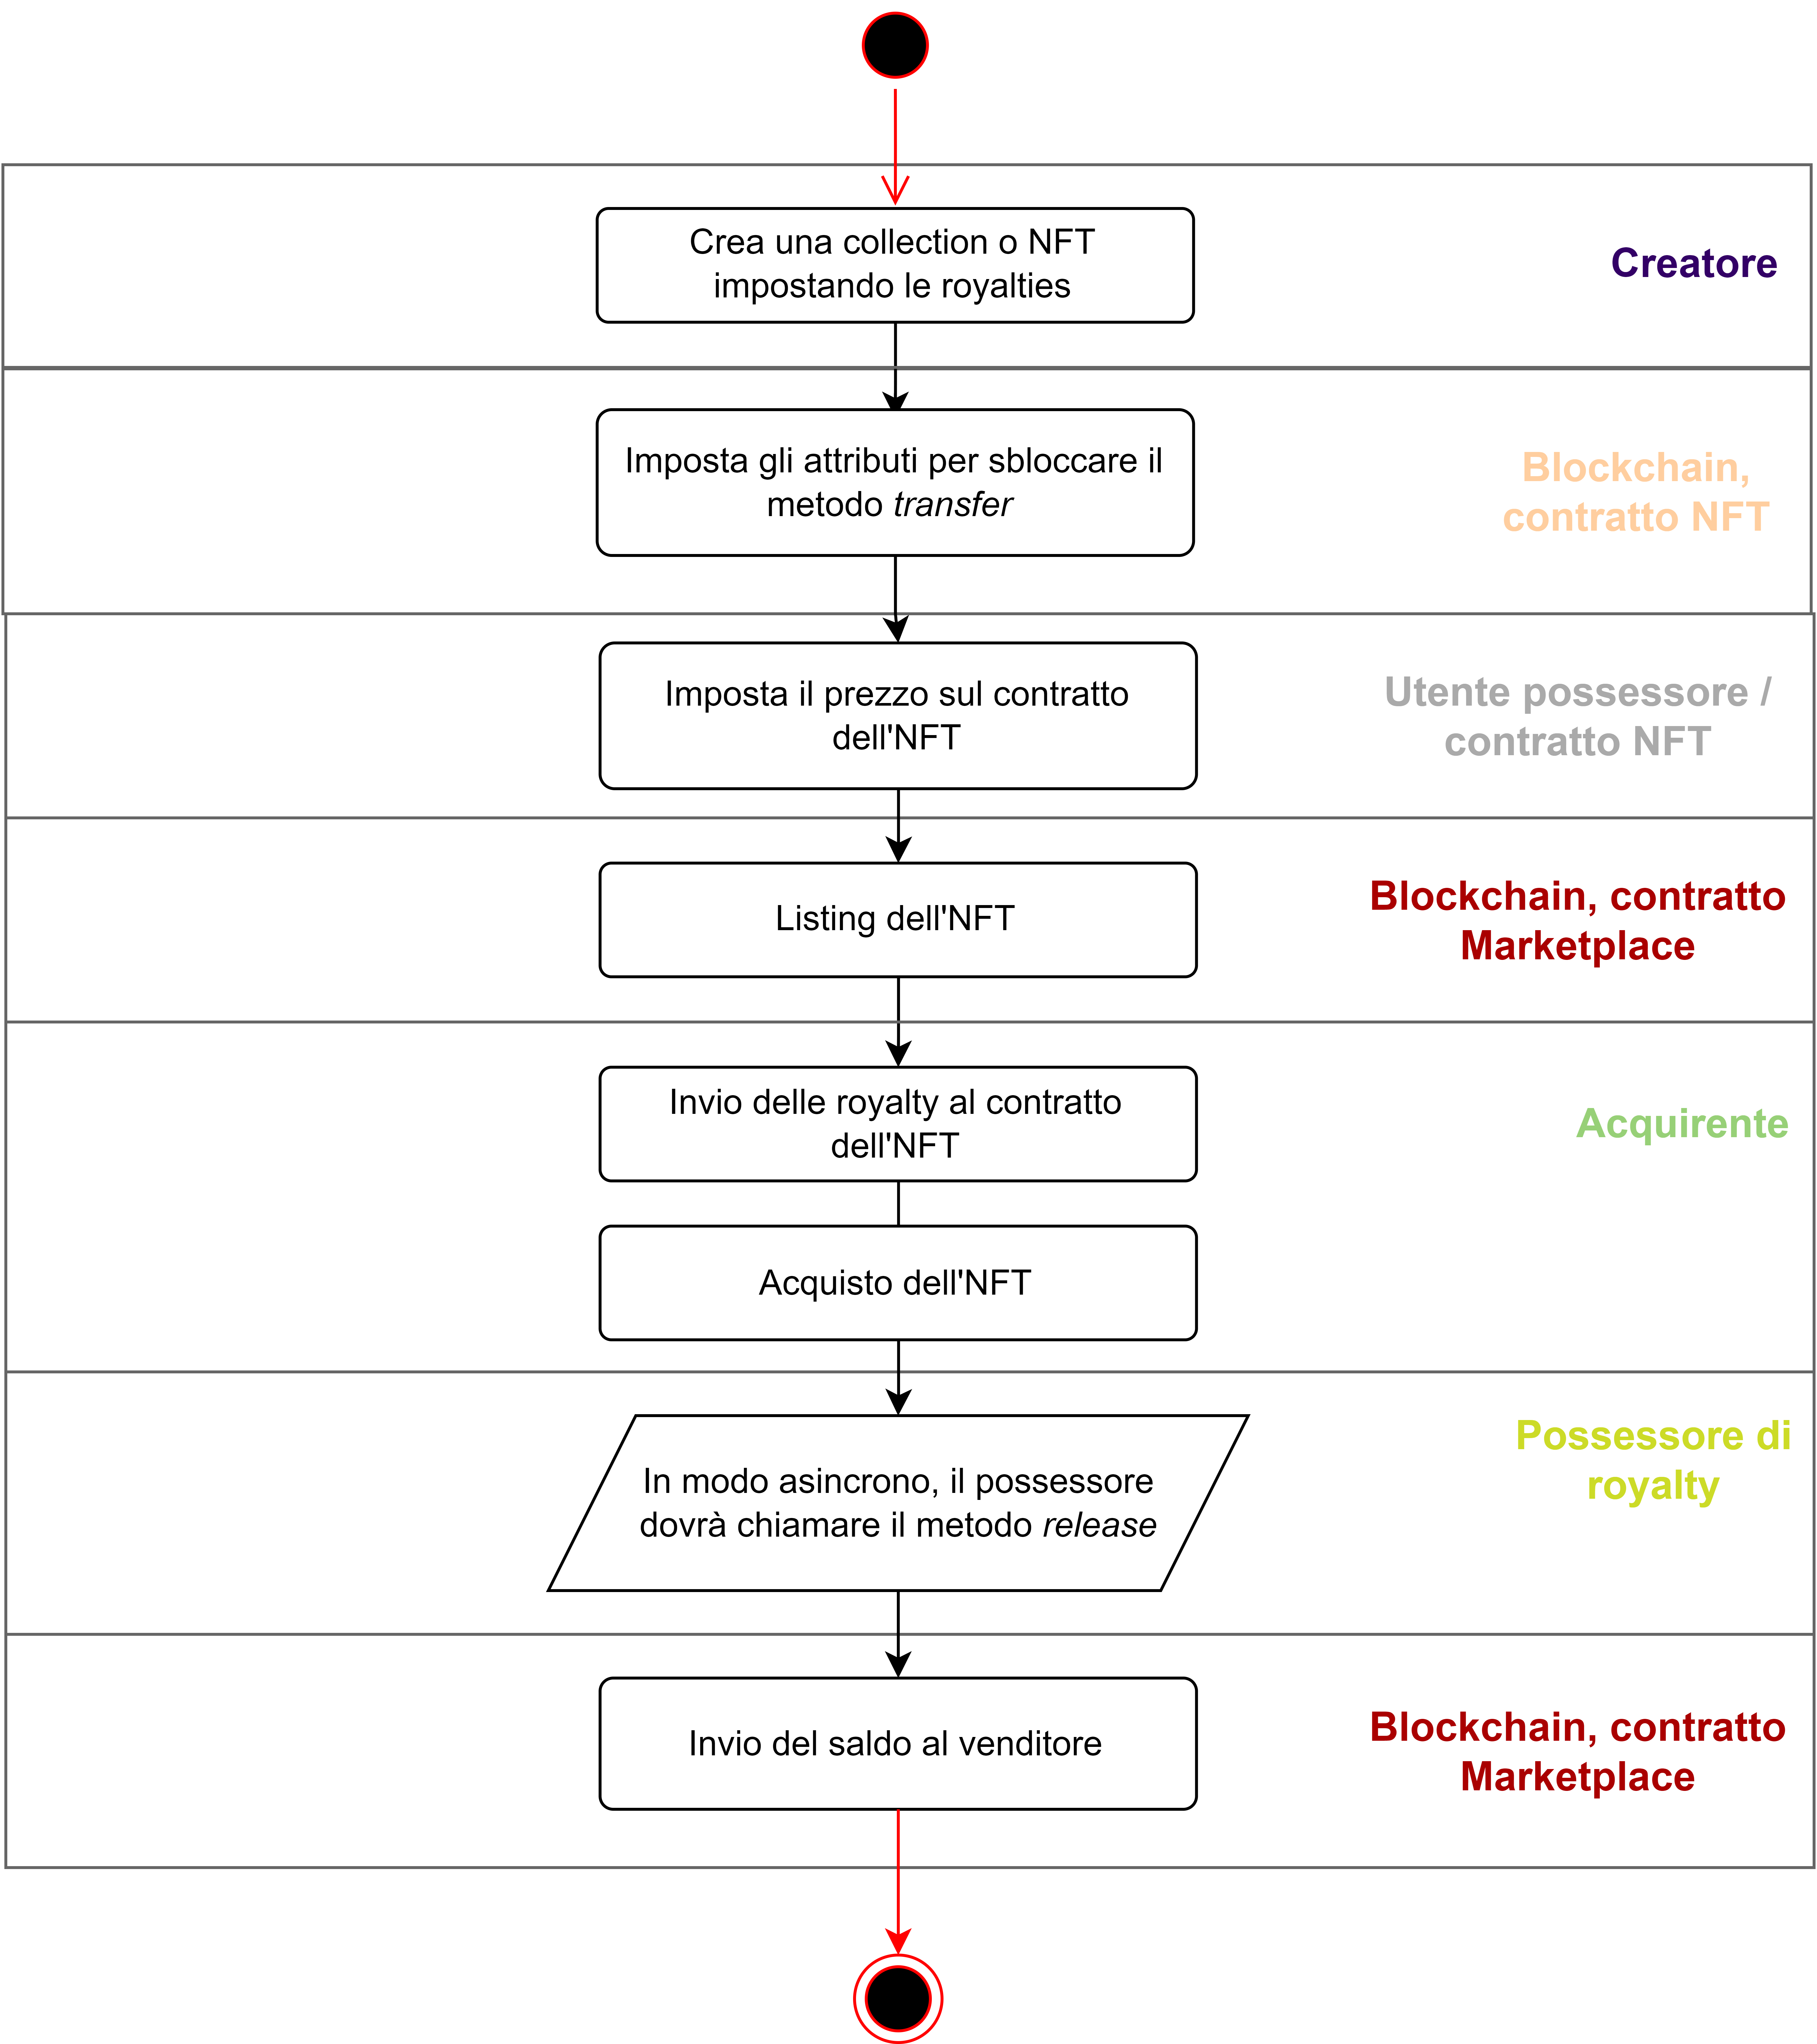
\includegraphics[width=1\textwidth]{images/creazioneVenditaNFTOverride.png}
    \caption{processo di creazione e vendita di un NFT con override del metodo transfer}
    \label{fig:creazioneVenditaNFTOverride}
\end{figure}

\newpage
\section{Architettura}
\label{sec:architettura}

Di seguito viene presentata l'architettura del sistema prodotto. La figura \ref{fig:architettura} mostra come le varie componenti interagiscono tra loro.

\begin{figure}[H]
    \centering
    \includegraphics[width=1.0\textwidth]{images/infrastruttura}
    \caption{Architettura del sistema}
    \label{fig:architettura}
\end{figure}

Come si può notare il sistema è composto da diversi componenti chiave. 

Il \textit{frontend} è stato sviluppato utilizzando il framework \textit{React} e il linguaggio di programmazione \textit{Typescript}. Esso si occupa di gestire l'interazione con l'utente, in particolare si occupa di richiedere i dati al backend e di mostrare all'utente le varie informazioni, nonché di inviare le richieste di interazione alla blockchain.

Come è osservabile dalla figura \ref{fig:architettura}, il frontend comunica con il backend tramite delle API di tipo GraphQL. Queste API sono state sviluppate utilizzando il framework \textit{Django} e il linguaggio di programmazione \textit{Python}. Il backend si occupa di gestire le richieste provenienti dal frontend, ovvero di recuperare i dati presenti nella blockchain e nel database, nonché di elaborarli e restituirli al frontend.

Tramite l'utilizzo del framework \textit{Hardhat} è stato possibile sviluppare gli smart contracts, i quali sono stati scritti utilizzando il linguaggio 
\textit{Solidity}. Inoltre, sono stati compilati e distribuiti sulla blockchain di test \textit{Sepolia}. Essi si occupano di gestire la logica di \textit{business}, in particolare la creazione, modifica e vendita di un asset, nonché la gestione del revenue share. In aggiunta, il framework permette di creare un'istanza di un nodo locale, così da poter utilizzare una blockchain locale.

Infine, il database è \textit{MongoDB}, ovvero un database di tipo \textit{NoSQL} basato su documenti. All'interno di esso vengono salvati unicamente alcuni dati di personalizzazione utente del marketplace.

In figura \ref{fig:architettura}, sono presenti due frecce tratteggiate, di seguito la loro spiegazione:
\begin{itemize}
    \item \textit{(1)}: L'esperienza utente è completamente compatibile sia con \textit{Desktop Browser} che con \textit{Mobile Browser}, tuttavia la connessione di un \textit{wallet} su \textit{Mobile Browser} presenta una funzionalità ridotta. La causa potrebbe essere dovuta da un problema di \textit{deep linking mobile}, ovvero la possibilità di aprire una comunicazione diretta tra due applicazioni, in questo caso tra il \textit{wallet} e il \textit{browser}. Questo problema è stato riscontrato utilizzando il \textit{wallet} \textit{MetaMask} su dispositivo \textit{Android}. Una possibile soluzione è quella di mettere in sicurezza l'applicativo frontend tramite l'utilizzo di certificati, in modo da poter utilizzare il protocollo \textit{https}.  
    \item \textit{(2)}: Non è attualmente presente un database di \textit{caching} dei dati presenti nella blockchain. In caso di forte utilizzo del marketplace in una blockchain pubblica e principale, come Ethereum mainnet, i tempi di risposta potrebbero essere molto alti. Perciò, sarebbe necessario implementare un database di questo tipo, un possibile candidato è \textit{Redis}.
\end{itemize}

Maggiori informazioni riguardo ad ogni componente e le motivazioni dietro le scelte effettuate sono presenti nei capitoli successivi.
\section{Blockchain}
\label{sec:blockchain-module}

Nel seguente capitolo viene descritto in maniera più approfondita il componente \textit{Blockchain}. In particolare, vengono analizzati gli smart contracts, i quali sono stati sviluppati utilizzando il framework \textit{Hardhat} e il linguaggio di programmazione \textit{Solidity} ma anche gli script utilizzati per l'automazione di alcune operazioni, i test effettuati e le possibili alternative.

\subsection{Smart contracts}
\label{sec:smart-contract-shopychange}

Per il corretto funzionamento del marketplace, sono stati sviluppati diversi smart contracts. In particolare, il contratto principale è \textit{ShopychangeMarketplace}, il quale si occupa di gestire la creazione, modifica, cancellazione e acquisto di una vendita. Inoltre, gestisce le \textit{royalty} e fornisce delle funzionalità di controllo per gli amministratori.

In aggiunta, il contratto \textit{ERC721 Factory} offre la possibilità di creazione di nuovi smart contracts di tipo \textit{ERC721} utilizzando un \textit{template} chiamato \textit{Boilerplate ERC721}. 

Infine, lo \textit{smart contract} \textit{Storage} viene utilizzato dagli utenti che non hanno necessità di creare una nuova collezione ma di generare un singolo asset.  

Nei prossimi capitoli verranno analizzati in dettaglio i contratti che compongono il marketplace. Di seguito, a figura \ref{fig:legenda}, è osservabile una legenda per la comprensione dei diagrammi.
\begin{figure}[H]
    \centering
    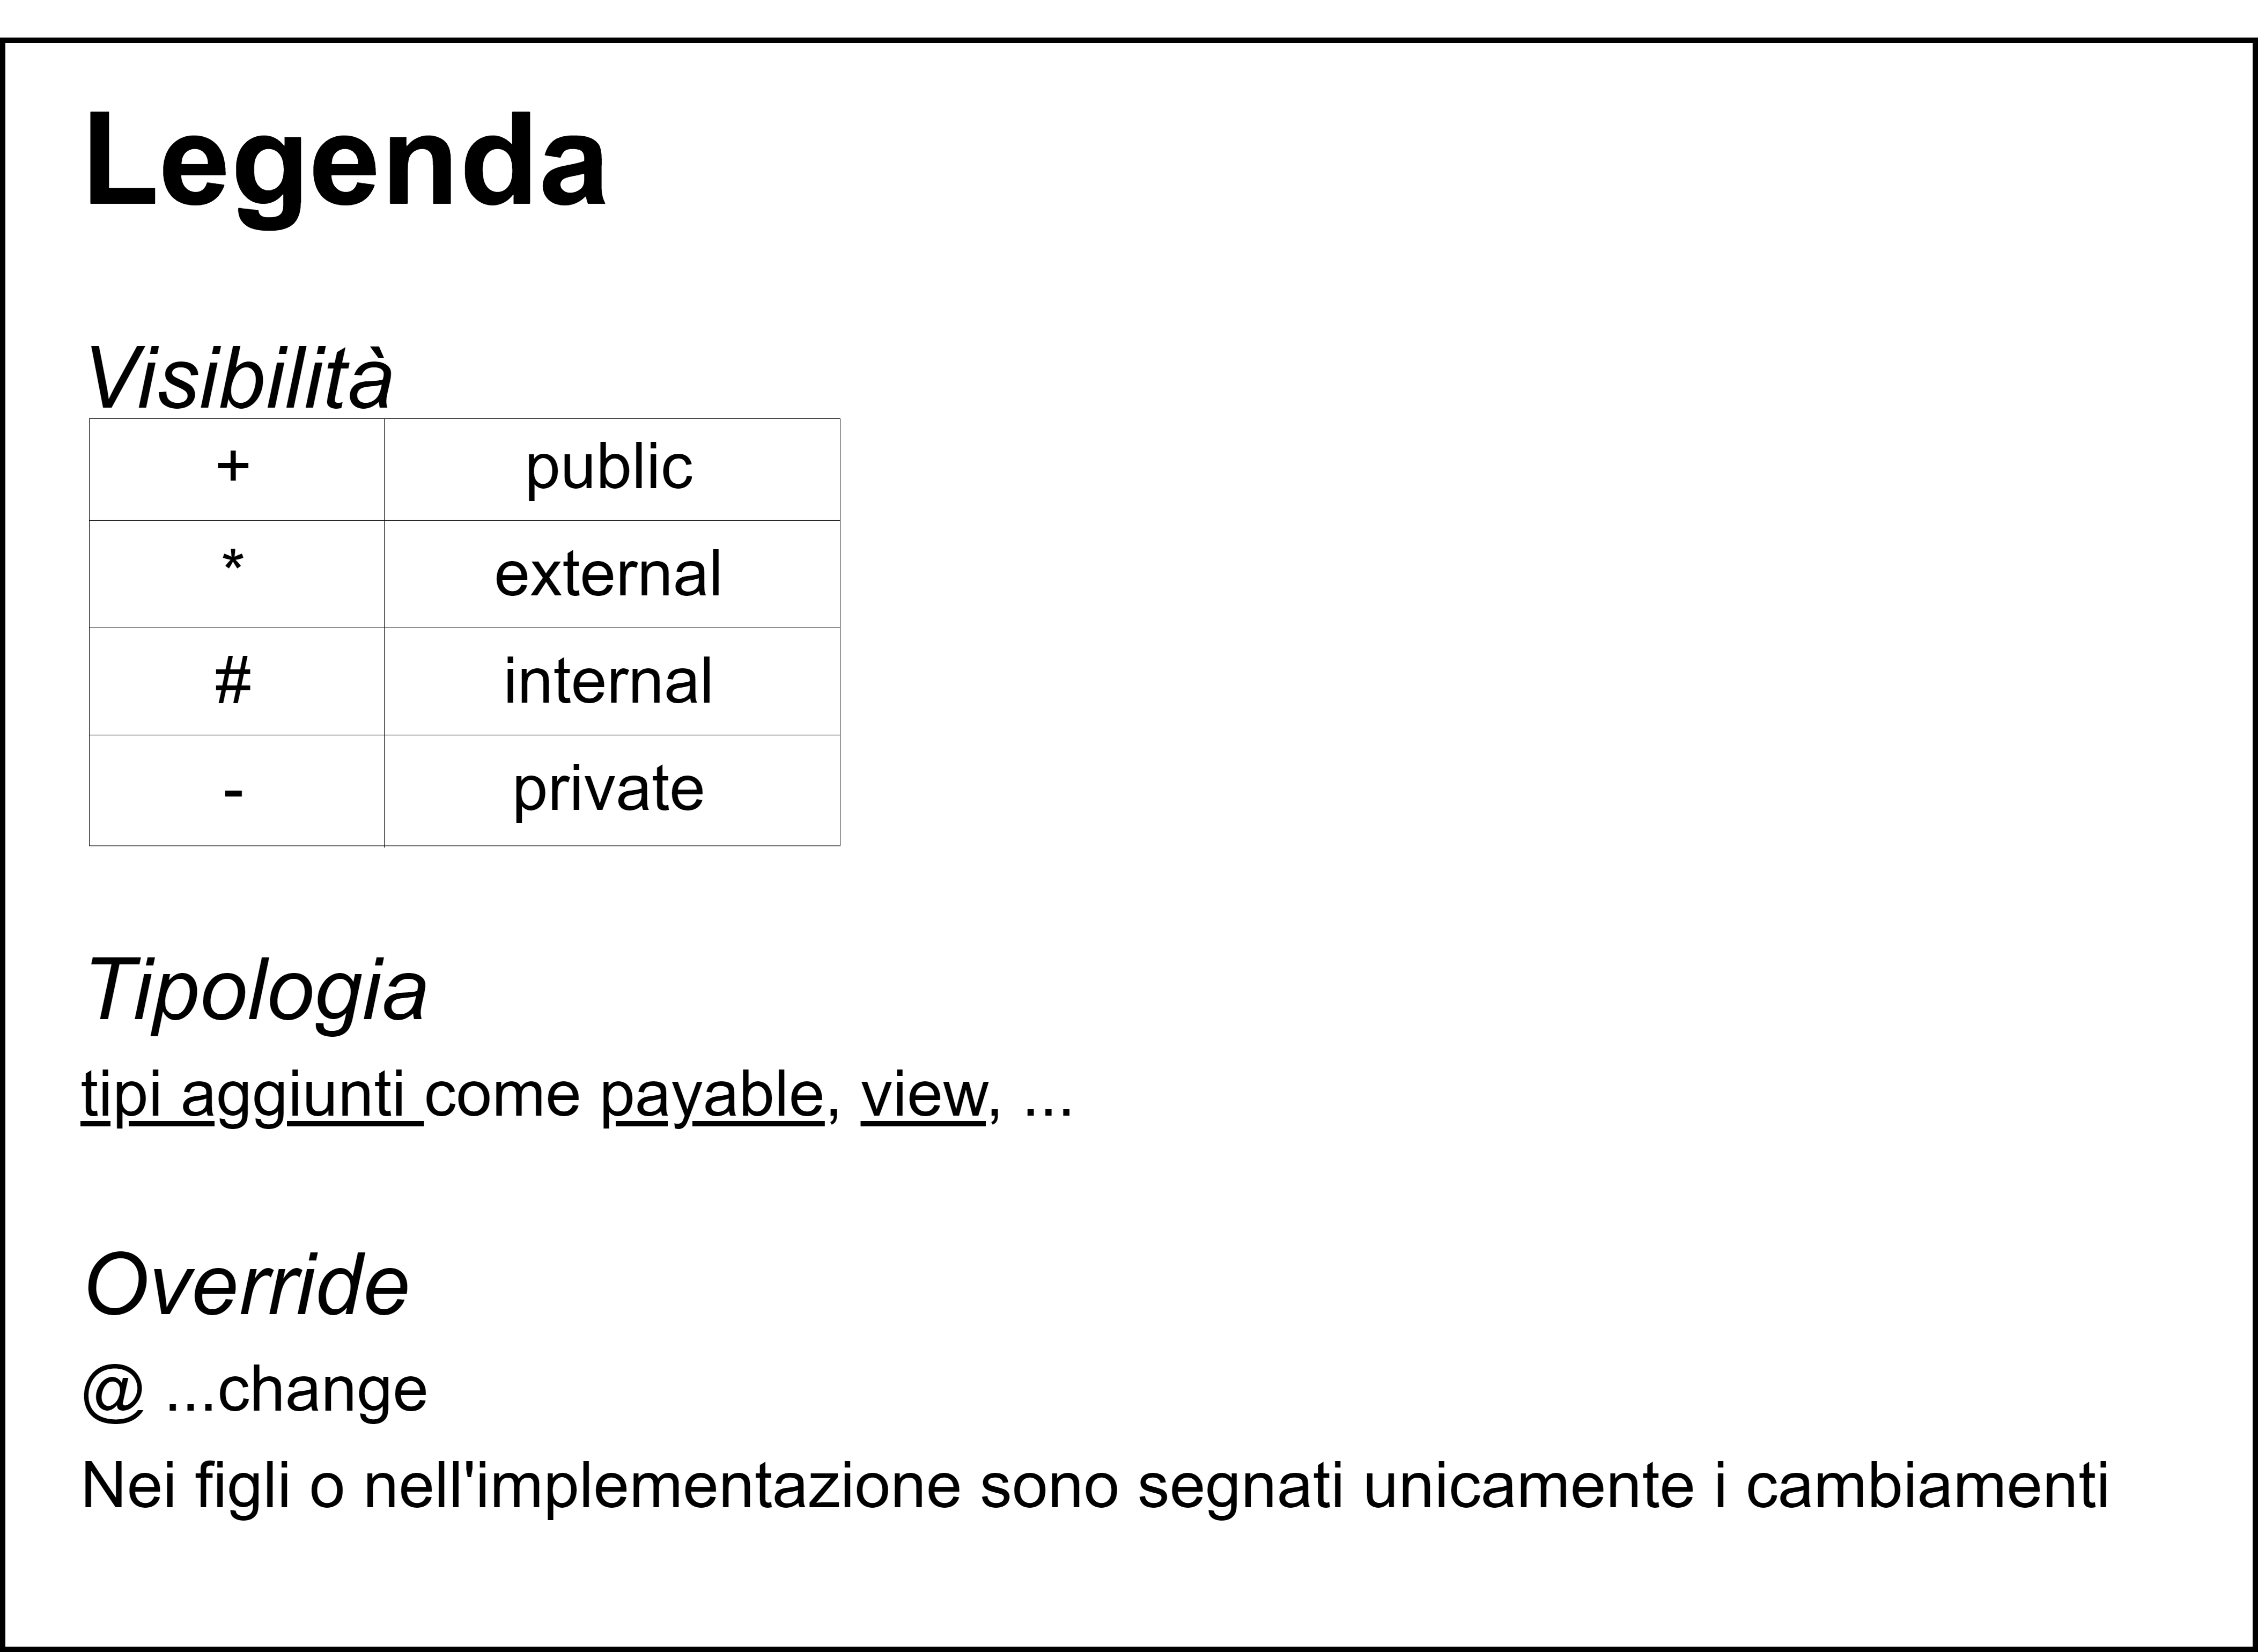
\includegraphics[width=0.8\textwidth]{images/blockchainContracts/LegendaBordo.png}
    \caption{Legenda Smart contracts}
    \label{fig:legenda}
\end{figure}

\subsubsection{Marketplace}

Il contratto \textit{core} del marketplace è \textit{ShopychangeMarketplace}. Per la sua realizzazione è stato deciso di utlizzare un approccio simile allo standard \textit{ERC721}, ovvero separando la logica in più contratti per facilitare la manutenzione, comprensione e testabilità del codice. Inoltre, grazie alla struttura a modelli è possibile decidere quali funzionalità abilitare o meno. Il contratto \textit{ShopychangeMarketplace} possiede tutte le funzionalità. La figura \ref{fig:marketplaceContract} mostra il diagramma UML del contratto.

\begin{figure}[H]
    \centering
    \includegraphics[width=1\textwidth]{images/blockchainContracts/ShopychangeMarketplaceReduced.png}
    \caption{Diagramma smart contract ShopychangeMarketplace}
    \label{fig:marketplaceContract}
\end{figure}


\paragraph{Fundamental}

Come si può osservare dalla figura \ref{fig:marketplaceFundamental}, il contratto \textit{MarketplaceFundamental} eredita dall'interfaccia \textit{IMarketplaceFundamental}. Questa interfaccia definisce le funzionalità obbligatorie del contratto \textit{Fundamental}, ovvero la creazione e acquisto di una vendita. Le informazioni relative alla vendita sono salvate in una struttura dati chiamata \textit{Sale}. Più in dettaglio, la struttura dati contiene le seguenti informazioni:

\begin{itemize}
    \item \textit{contractAddress}: indirizzo del contratto che rappresenta la collezione
    \item \textit{tokenId}: identificativo dell'asset all'interno della collezione
    \item \textit{price}: prezzo di vendita
    \item \textit{seller}: indirizzo del venditore
    \item \textit{status}: stato della vendita, può essere \textit{None} = 0 (Non presente nel marketplace), \textit{Cancelled} = 1 (Cancellata), \textit{Sold} = 2 (Venduta), \textit{Listed} = 3 (In vendita)
\end{itemize}

Gli attributi \textit{\_sales} e \textit{\_salesIds} presenti nel contratto \textit{MarketplaceFundamental} sono utilizzati per mantenere le informazioni relative alle vendite. In maniera più approfondita, \textit{\_sales} è una \textit{map} che associa ad ogni identificativo di una vendita la struttura dati \textit{Sale}. Mentre, \textit{\_salesIds} è un array che contiene gli identificativi delle vendite presenti nel marketplace. L'id in formato \textit{bytes32} è generato crittografando l'indirizzo del contratto e l'identificativo dell'asset, creando così un valore univoco per ogni vendita. L'id generato è ottenibile utilizzando la funzione \textit{getKey}. 

Nel momento in cui avviene la creazione di una vendita, lo smart contract controllerà che le informazioni fornite siano valevoli e che il chiamante sia effettivamente il possessore dell'asset. Un processo simili avviene anche all'acquisto del token, dove il contratto verifica che il \textit{seller} sia ancora il possessore. Maggiori dettagli su questa possibile situazioni sono presenti nel capitolo \hyperref[sec:controllo-integrita-nft-in-vendita]{\textit{Controllo integrità NFT in vendita}}.

Nel momento in cui avviene un acquisto, il metodo \textit{buy} eseguirà \textit{payShares}, questo meccanismo permetterà ai contratti figli di poter gestire le \textit{royalty} in maniera personalizzata. Maggiori informazioni nei capitoli \hyperref[sec:marketplace-earnable]{\textit{Earnable}} e \hyperref[sec:marketplace-royalty-applicable]{\textit{RoyaltyApplicable}}.

Infine, il contratto presenta alcune funzioni di tipo \textit{view}, le quali permettono di ottenere le vendite presenti nel marketplace.

\begin{figure}[H]
    \centering
    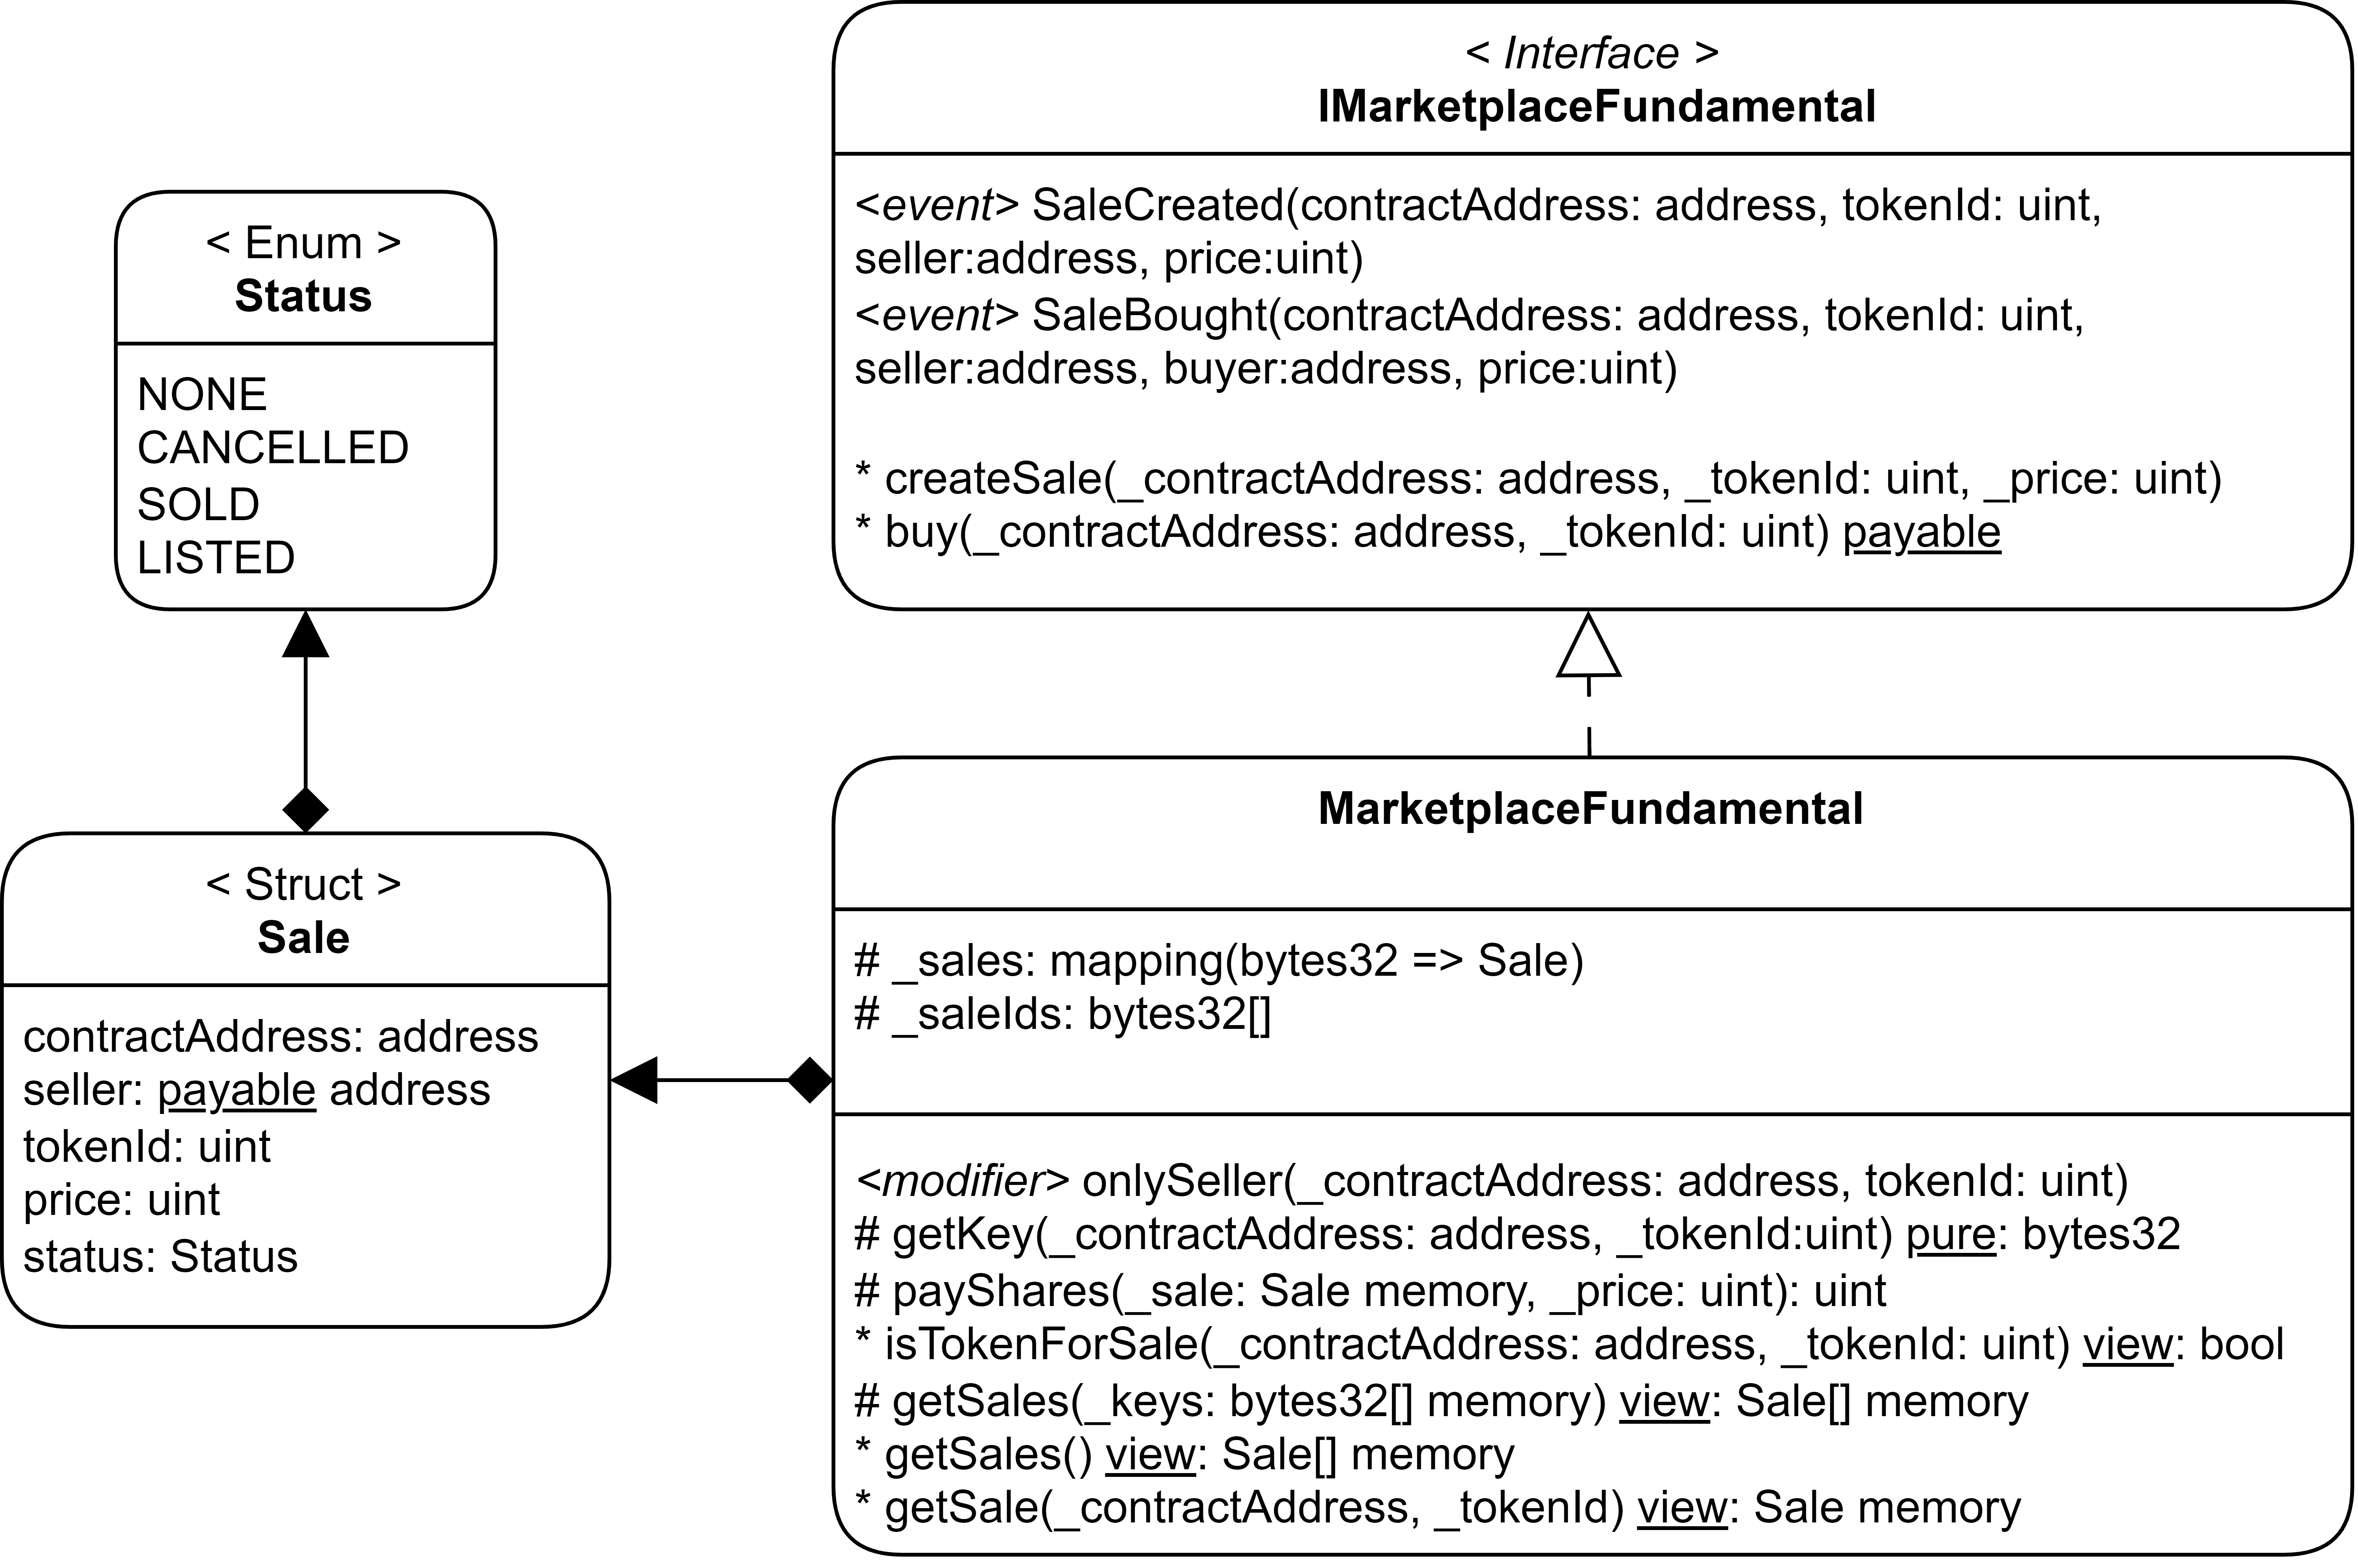
\includegraphics[width=1\textwidth]{images/blockchainContracts/MarketplaceFundamental.png}
    \caption{Marketplace Fundamental}
    \label{fig:marketplaceFundamental}
\end{figure}



\paragraph{Cancellable}
L'estensione \textit{Cancellable} permette la cancellazione di una vendita in corso. Nello specifico, il contratto \textit{MarketplaceCancellable} eredita da \textit{IMarketplaceCancellable} e \textit{MarketplaceFundamental}. Come visibile in figura \ref{fig:marketplaceCancellable} il contratto presenta la funzione \textit{cancelSale}, la quale è utilizzabile unicamente dal possessore dell'asset o dall'amministratore.

\begin{figure}[H]
    \centering
    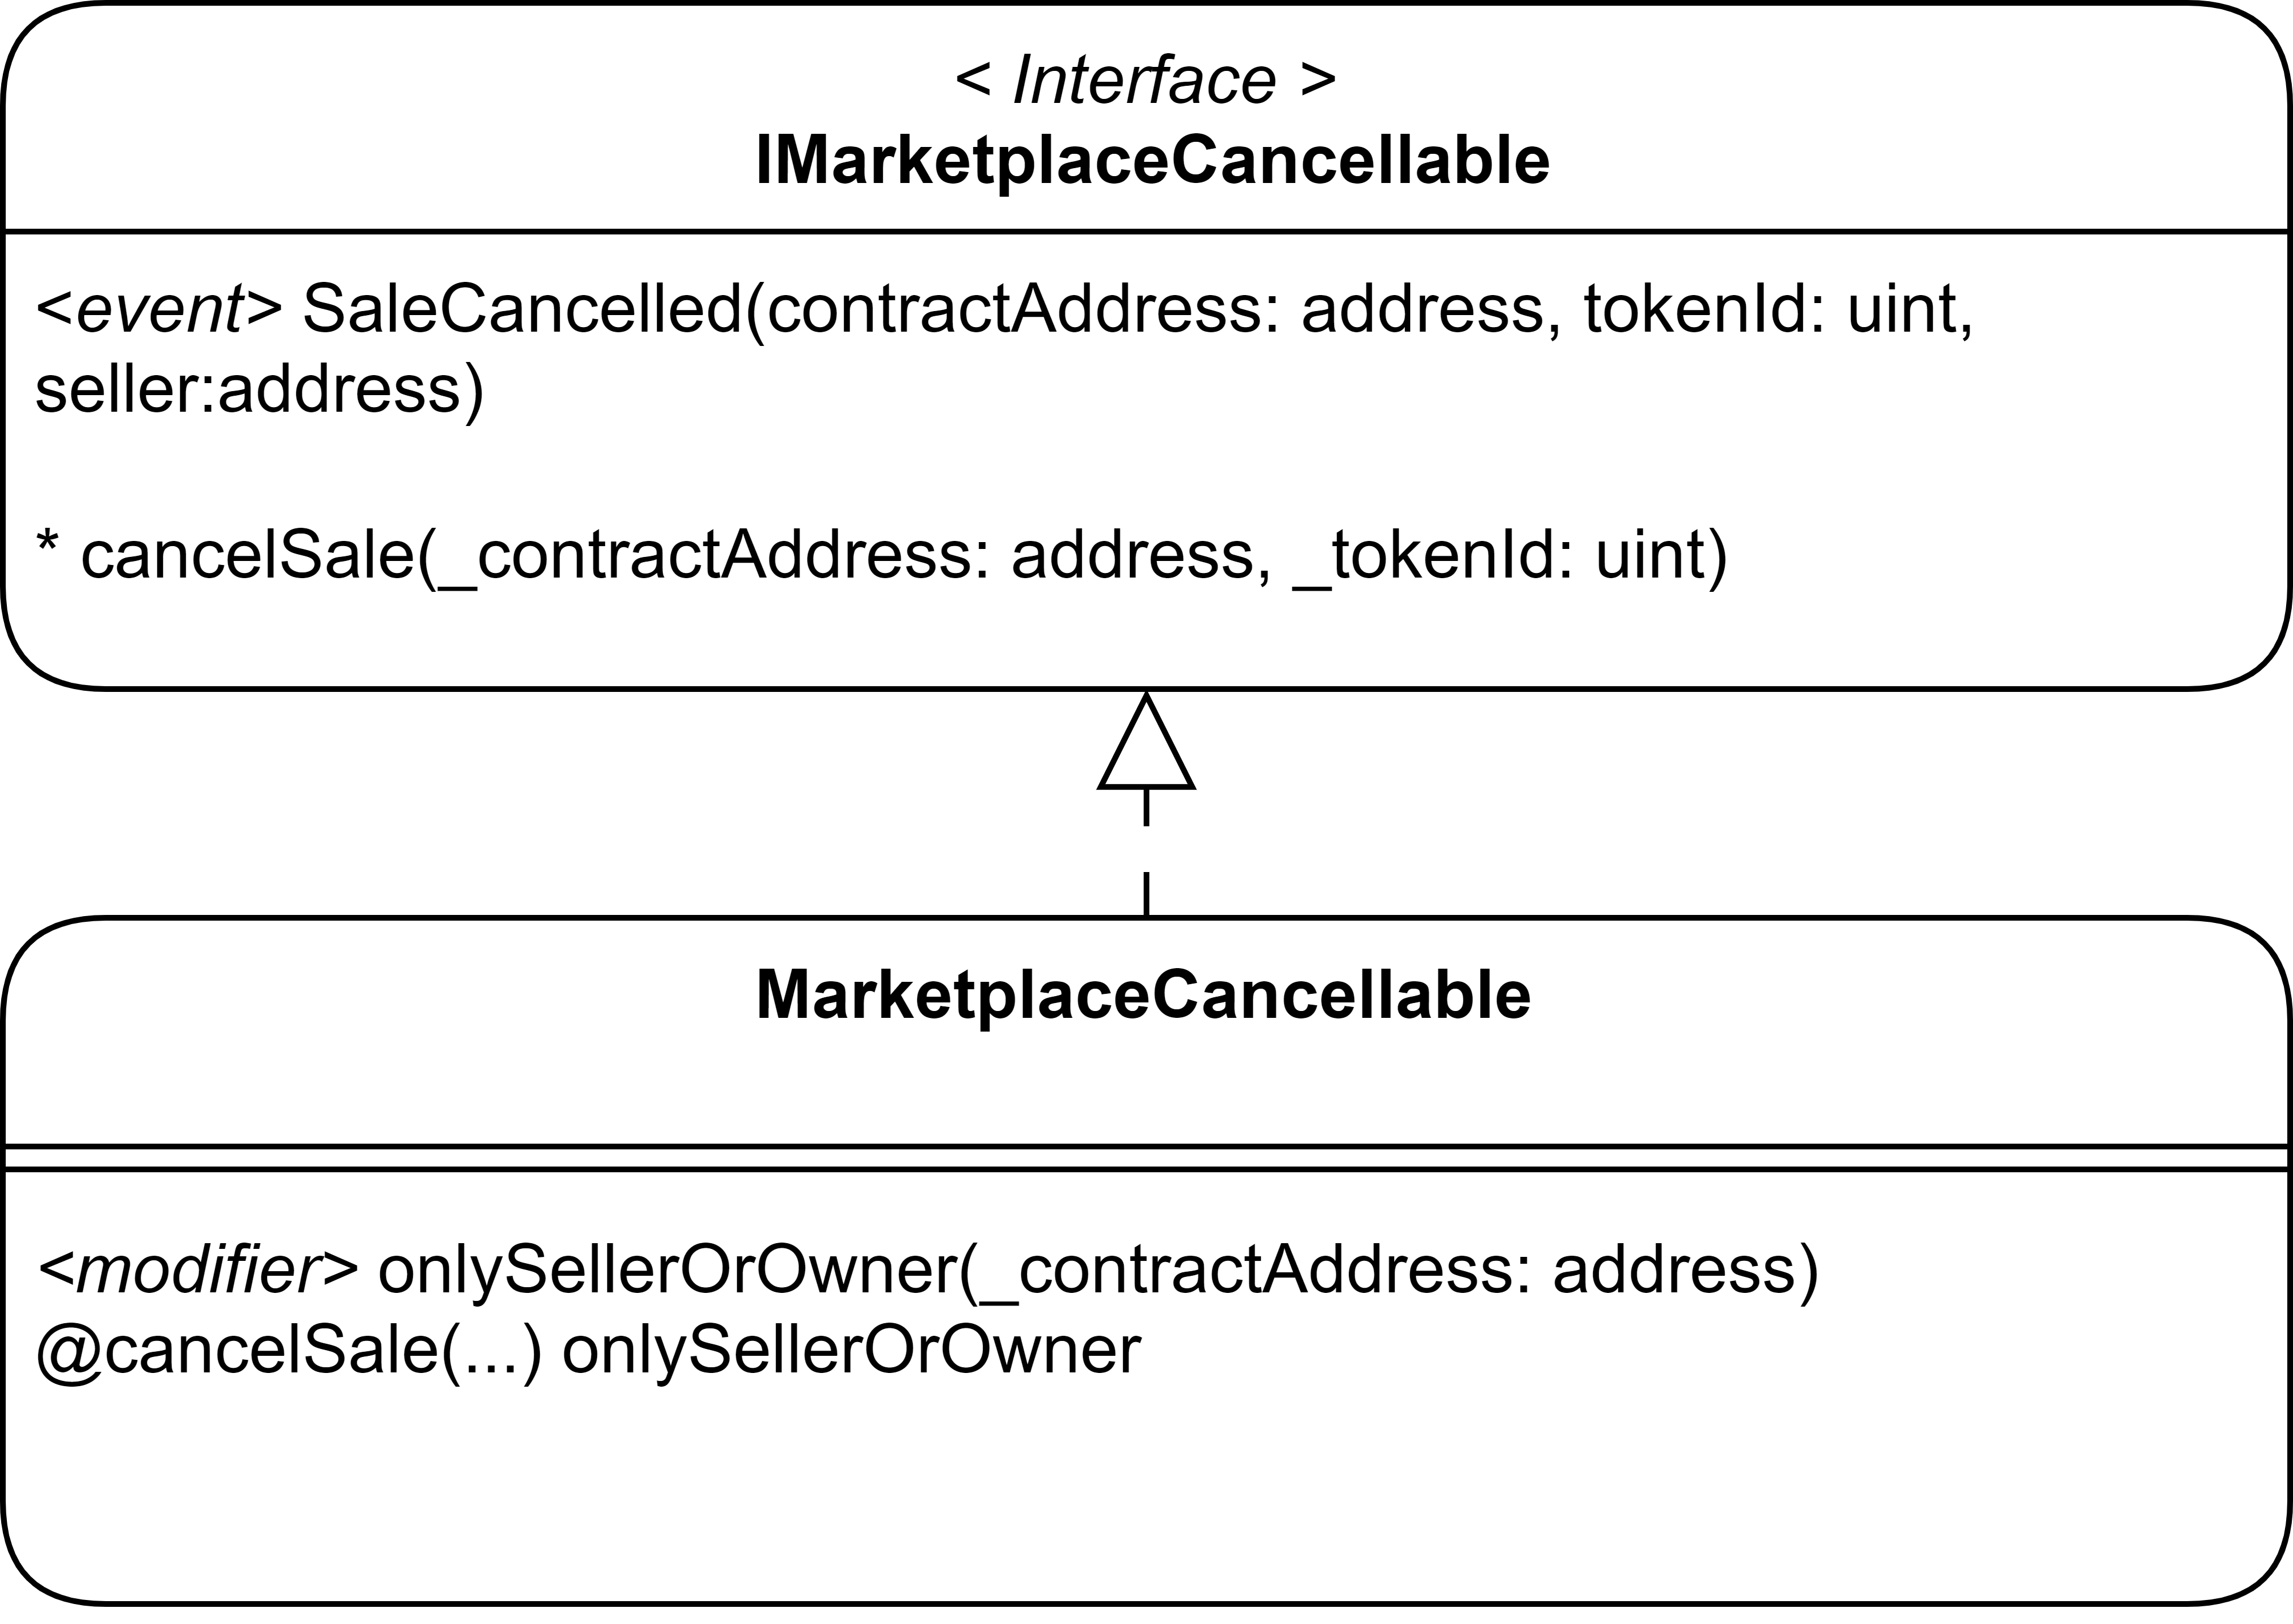
\includegraphics[width=0.7\textwidth]{images/blockchainContracts/MarketplaceCancellable.png}
    \caption{Marketplace Cancellable}
    \label{fig:marketplaceCancellable}
\end{figure}

\paragraph{Modifiable}
Il contratto \textit{MarketplaceModifiable} estende \textit{IMarketplaceModifiable} e \textit{IMarketplaceCancellable}. La sua funzione è quella di consentire la modifica del prezzo di vendita di un asset. Questa operazione è eseguibile unicamente dal possessore dell'asset, come visibile in figura \ref{fig:marketplaceModifiable}.

\begin{figure}[H]
    \centering
    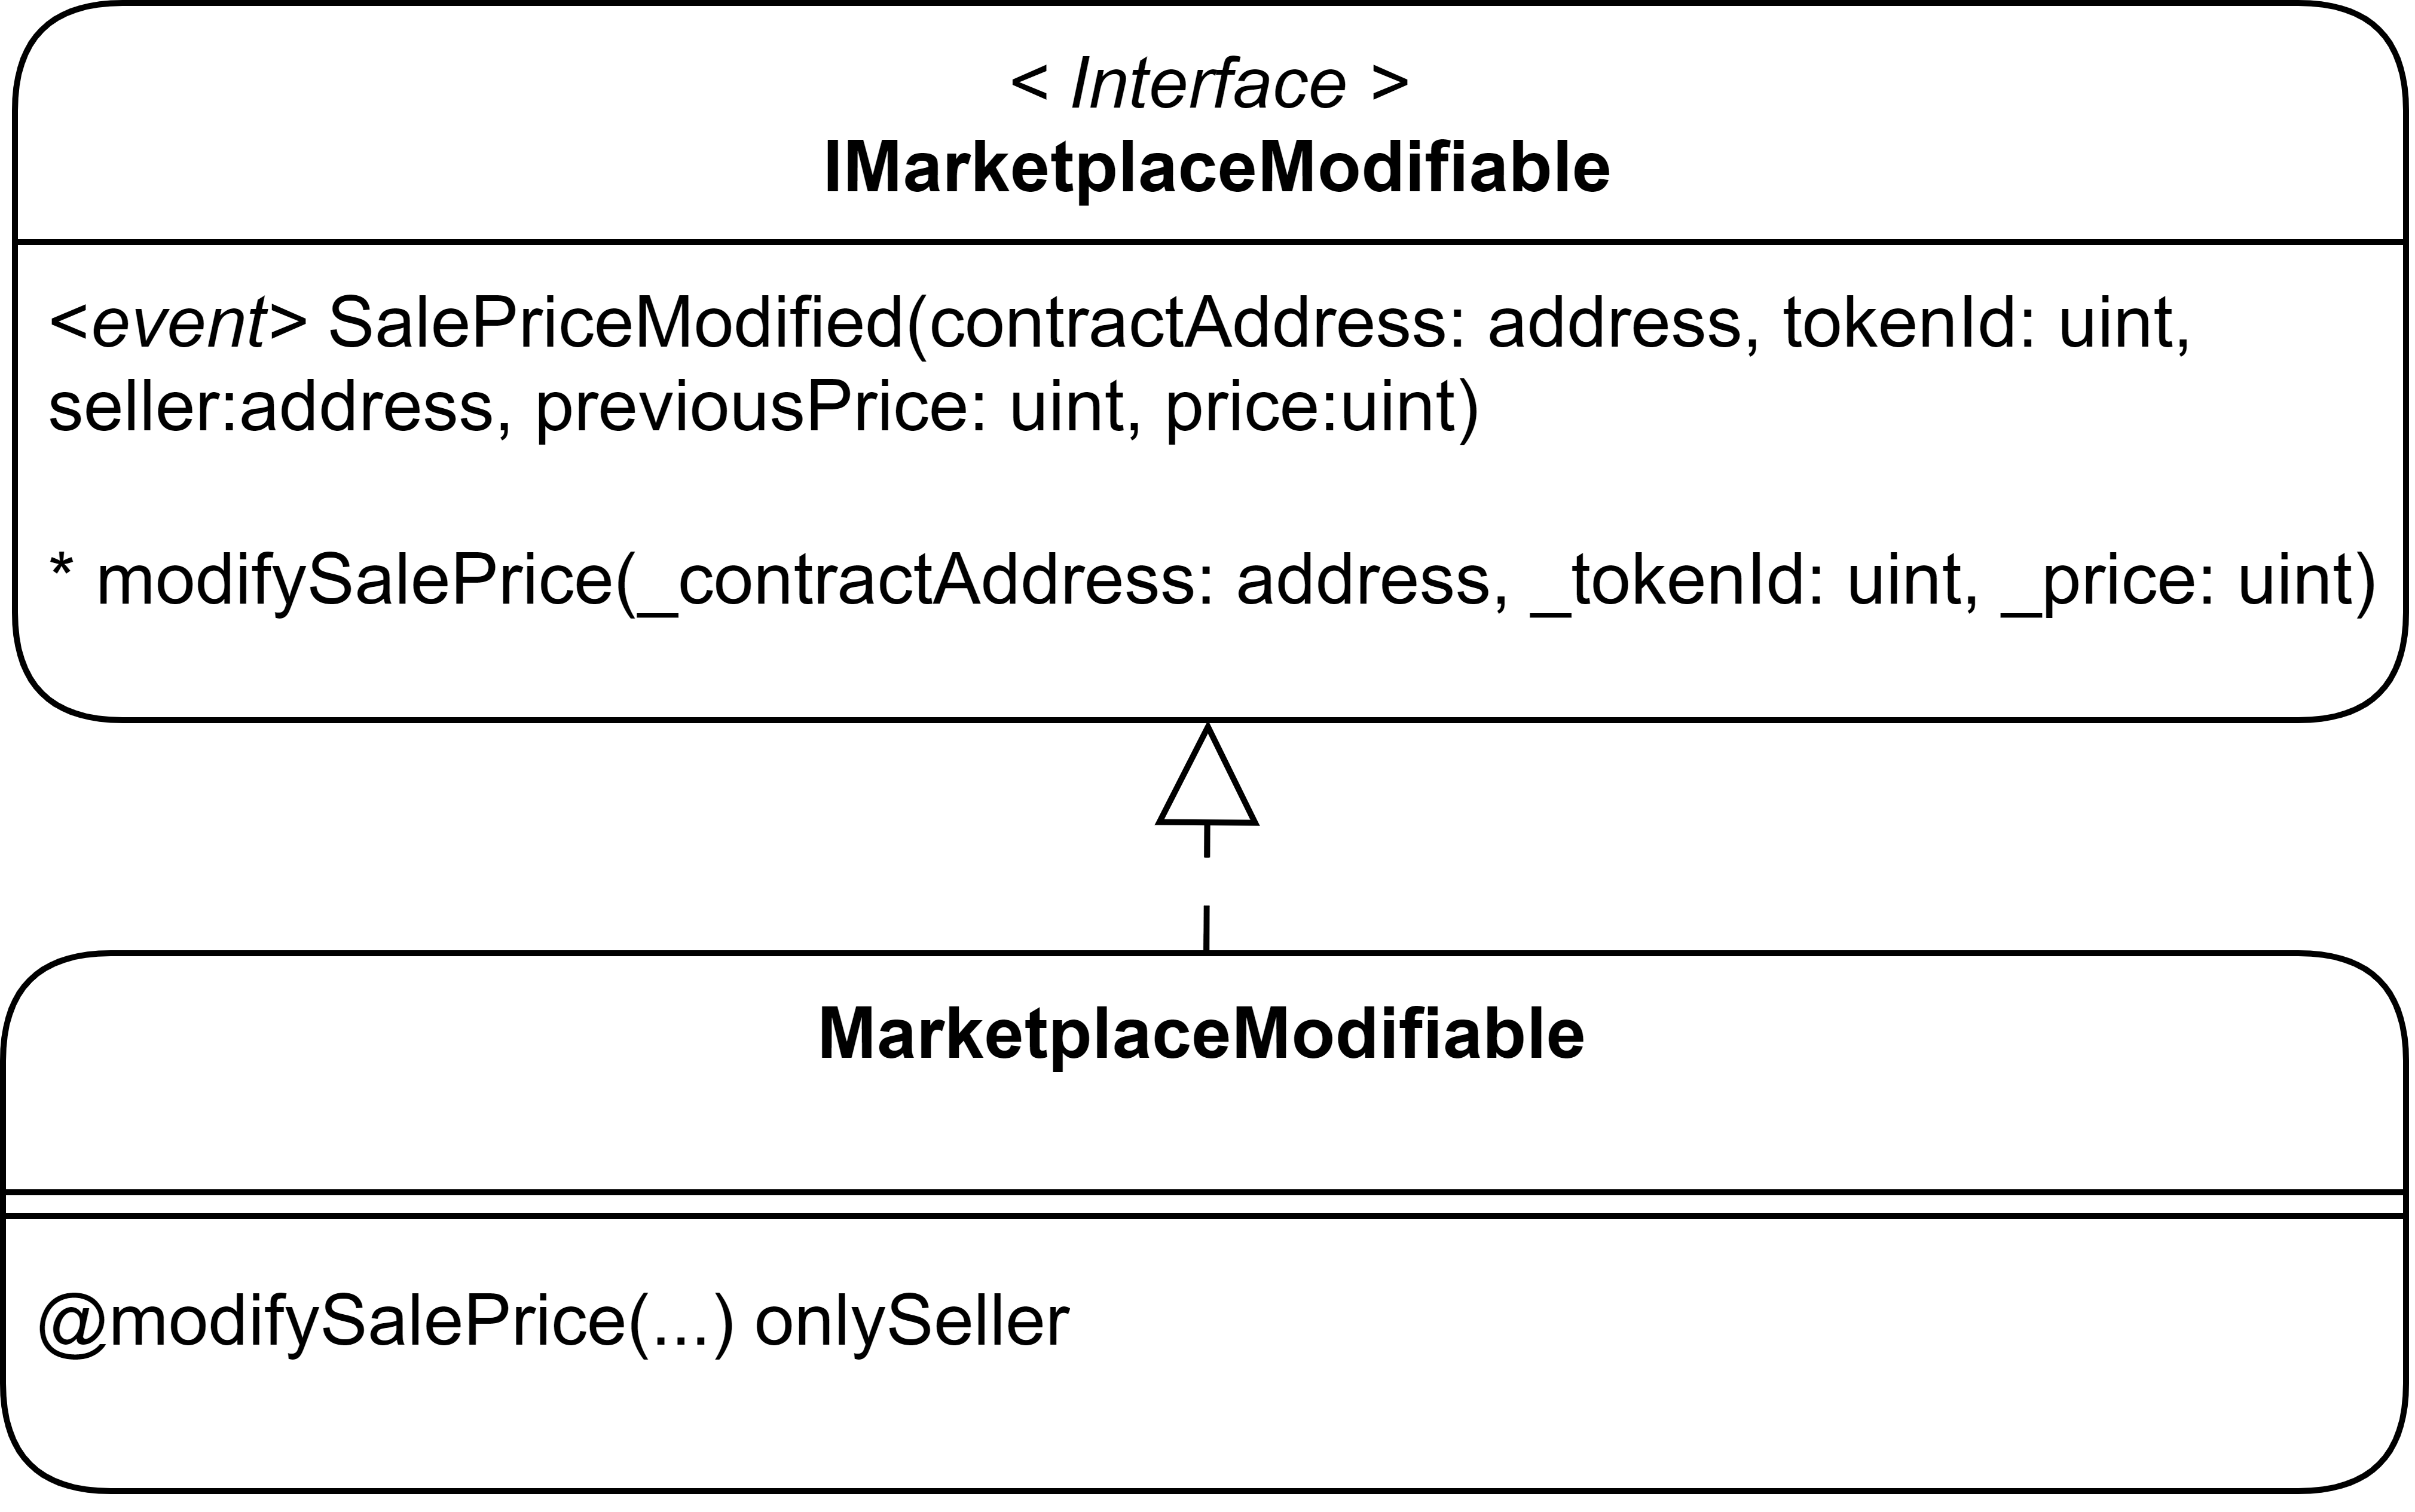
\includegraphics[width=0.7\textwidth]{images/blockchainContracts/MarketplaceModifiable.png}
    \caption{Marketplace Modifiable}
    \label{fig:marketplaceModifiable}
\end{figure}

\paragraph{Earnable}
\label{sec:marketplace-earnable}

Questo contratto consente il collezionamento di royalty a favore del marketplace per ogni acquisto effettuato. Come visibile in figura \ref{fig:marketplaceEarnable}, il contratto contiene il metodo \textit{receiver}, ovvero uno speciale metodo che permette al contratto di ricevere \textit{ETH}. La possibilità di collezionare le royalty è data dal metodo \textit{payShares}, il quale viene chiamato all'interno contratto \textit{MarketplaceFundamental}  nel momento in cui avviene un acquisto. 

Più in dettaglio, effettuando l'\textit{override} del metodo \textit{payShares}, che sarà chiamato dal metodo \textit{buy}, avviene una divisione del prezzo di vendita in base al valore presente nell'attributo \textit{royalty}. Questo valore rappresenta la percentuale di royalty che il marketplace riceverà per ogni acquisto, esso è un \textit{uint16} in quanto rappresenta un valore percentuale in \textit{basis point} (il valore 1 corrisponde allo 0.01\%, mentre il valore 10000 rappresenta il 100\%). In aggiunta, sono presenti alcune funzionalità di \textit{get} e \textit{set} per modificare il valore percentuale, nonchè diversi metodi per ritirare il saldo del contratto. 

\begin{figure}[H]
    \centering
    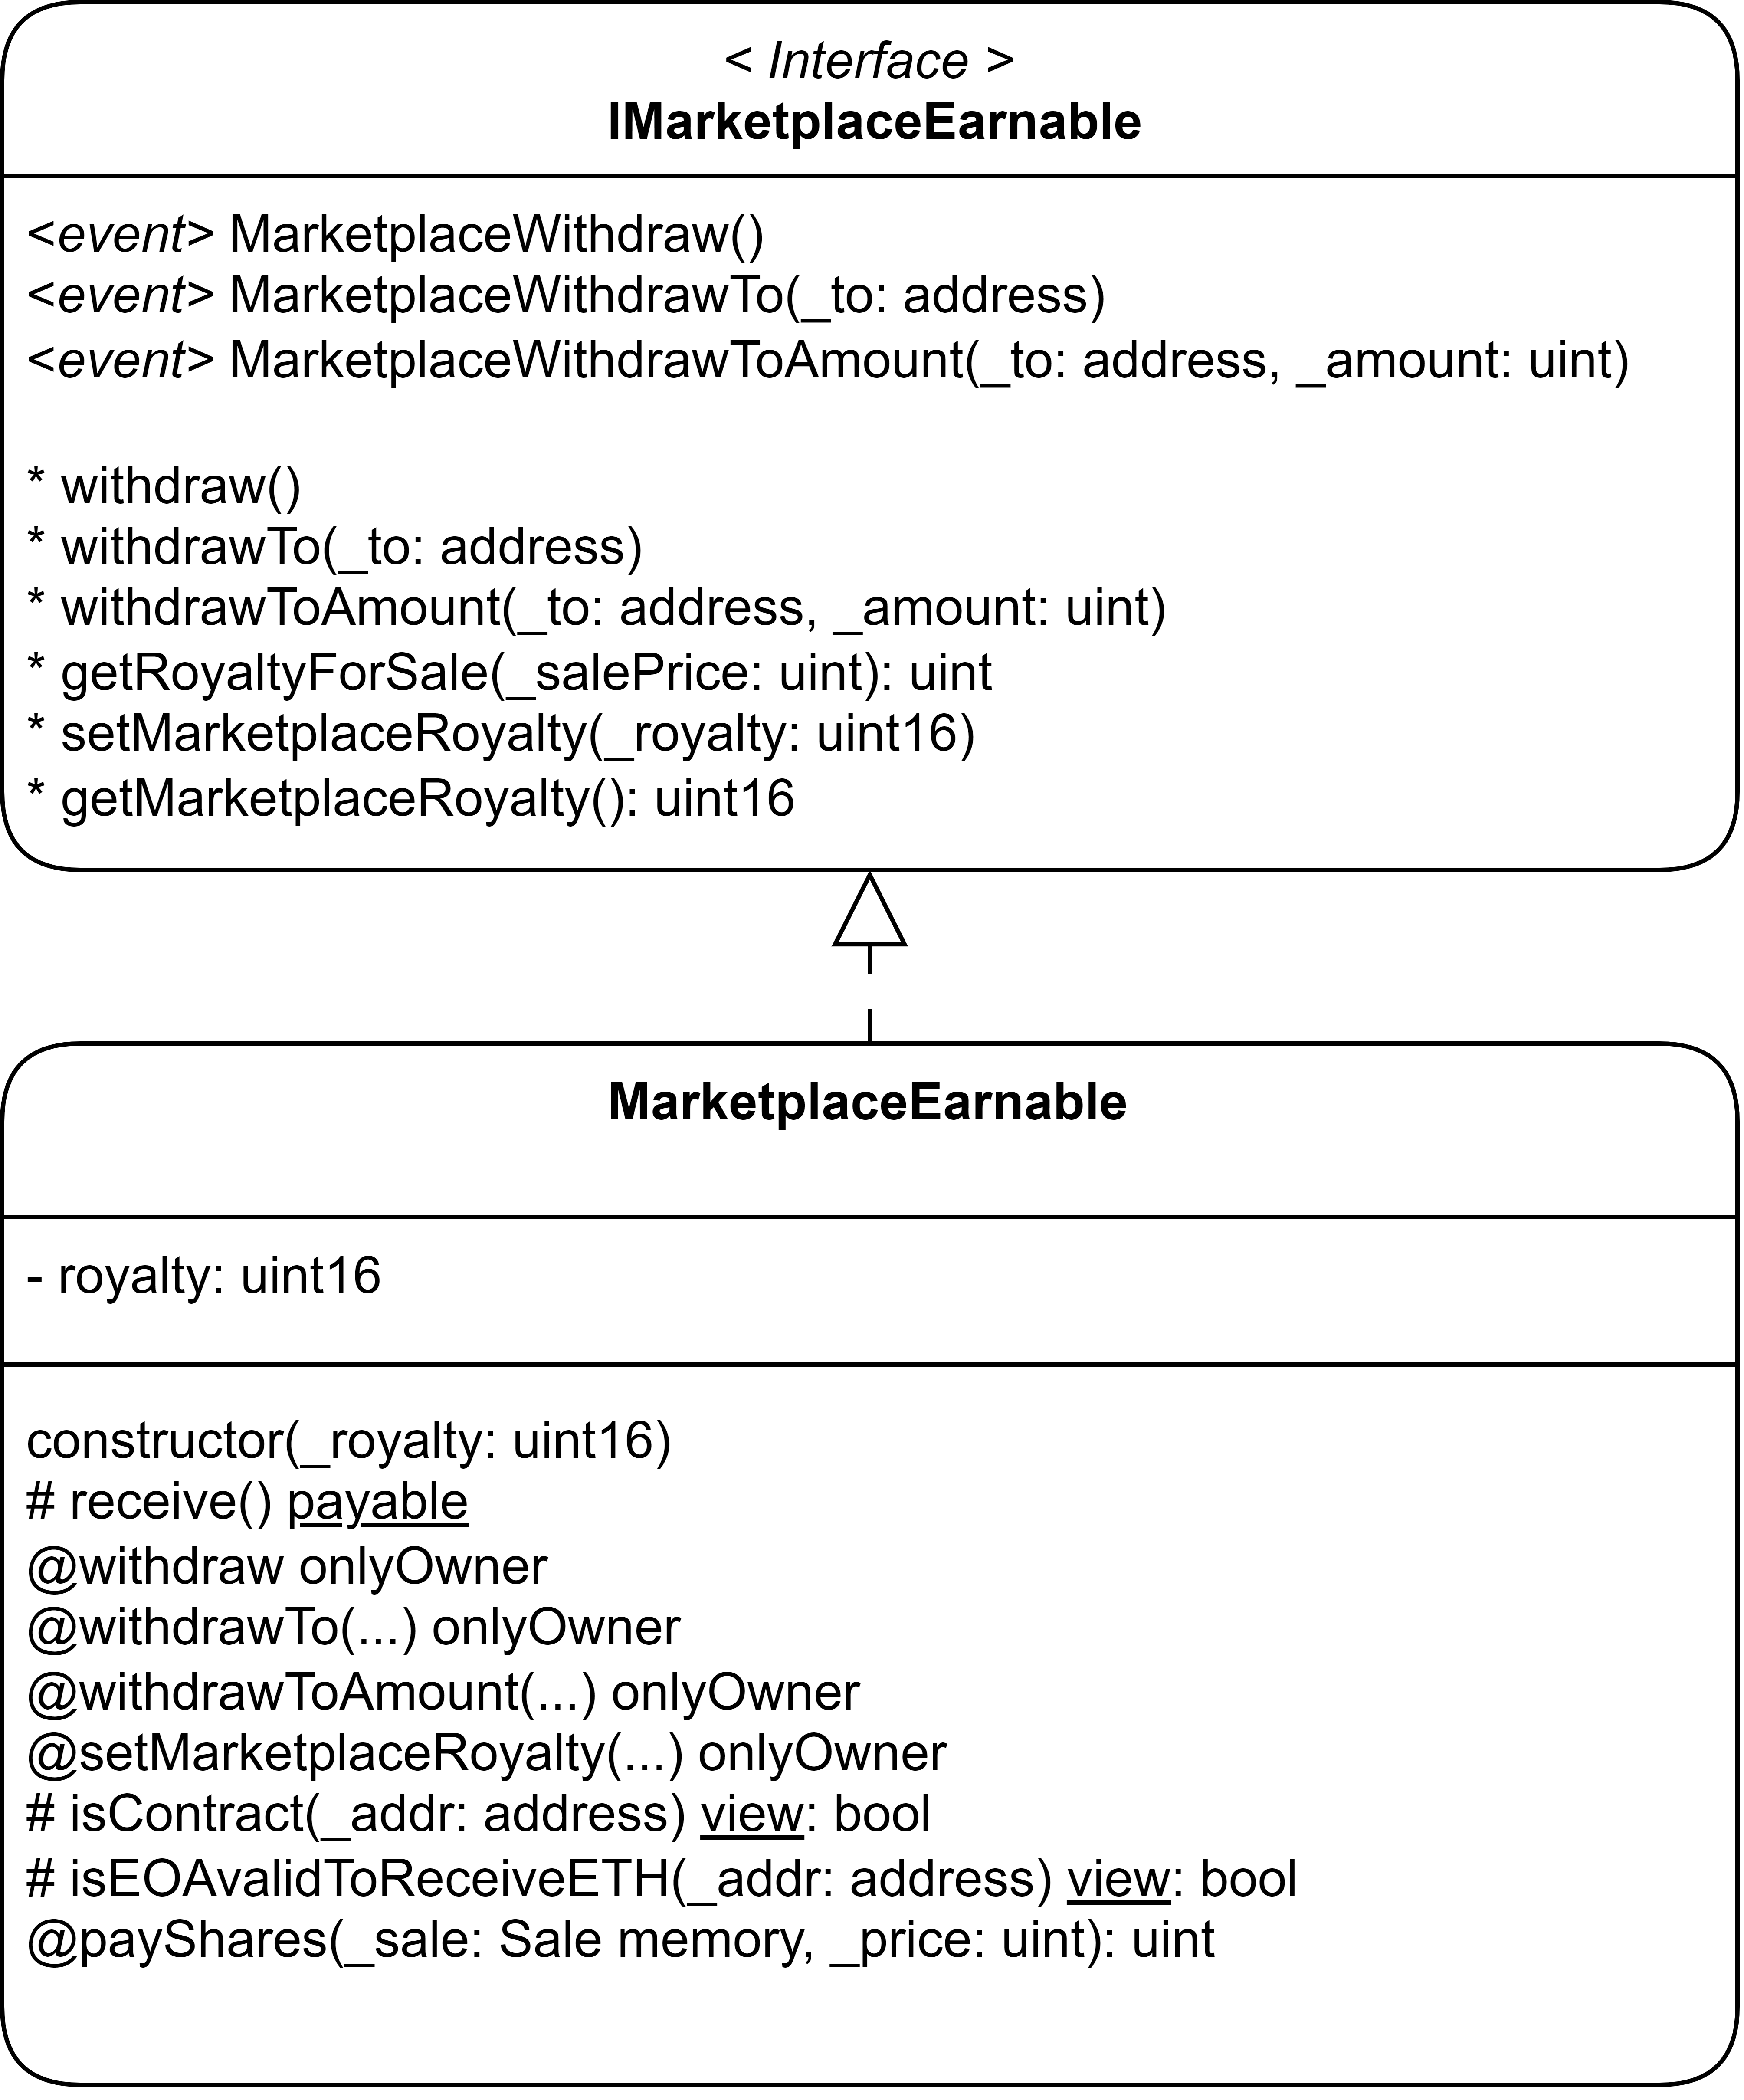
\includegraphics[width=0.7\textwidth]{images/blockchainContracts/MarketplaceEarnable.png}
    \caption{Marketplace Earnable}
    \label{fig:marketplaceEarnable}
\end{figure}

\paragraph{RoyaltyApplicable}
\label{sec:marketplace-royalty-applicable}

Il contratto \textit{RoyaltyApplicable} ha un funzionamento simile al contratto \hyperref[sec:marketplace-earnable]{\textit{Earnable}}. Ovvero, effettuando l'\textit{override} del metodo \textit{payShares} il saldo sarà diviso. In questo caso,
nel momento in cui avviene un acquisto il saldo inviato sarà separato tra il venditore e gli indirizzi definiti dal creatore dell'asset.

\begin{figure}[H]
    \centering
    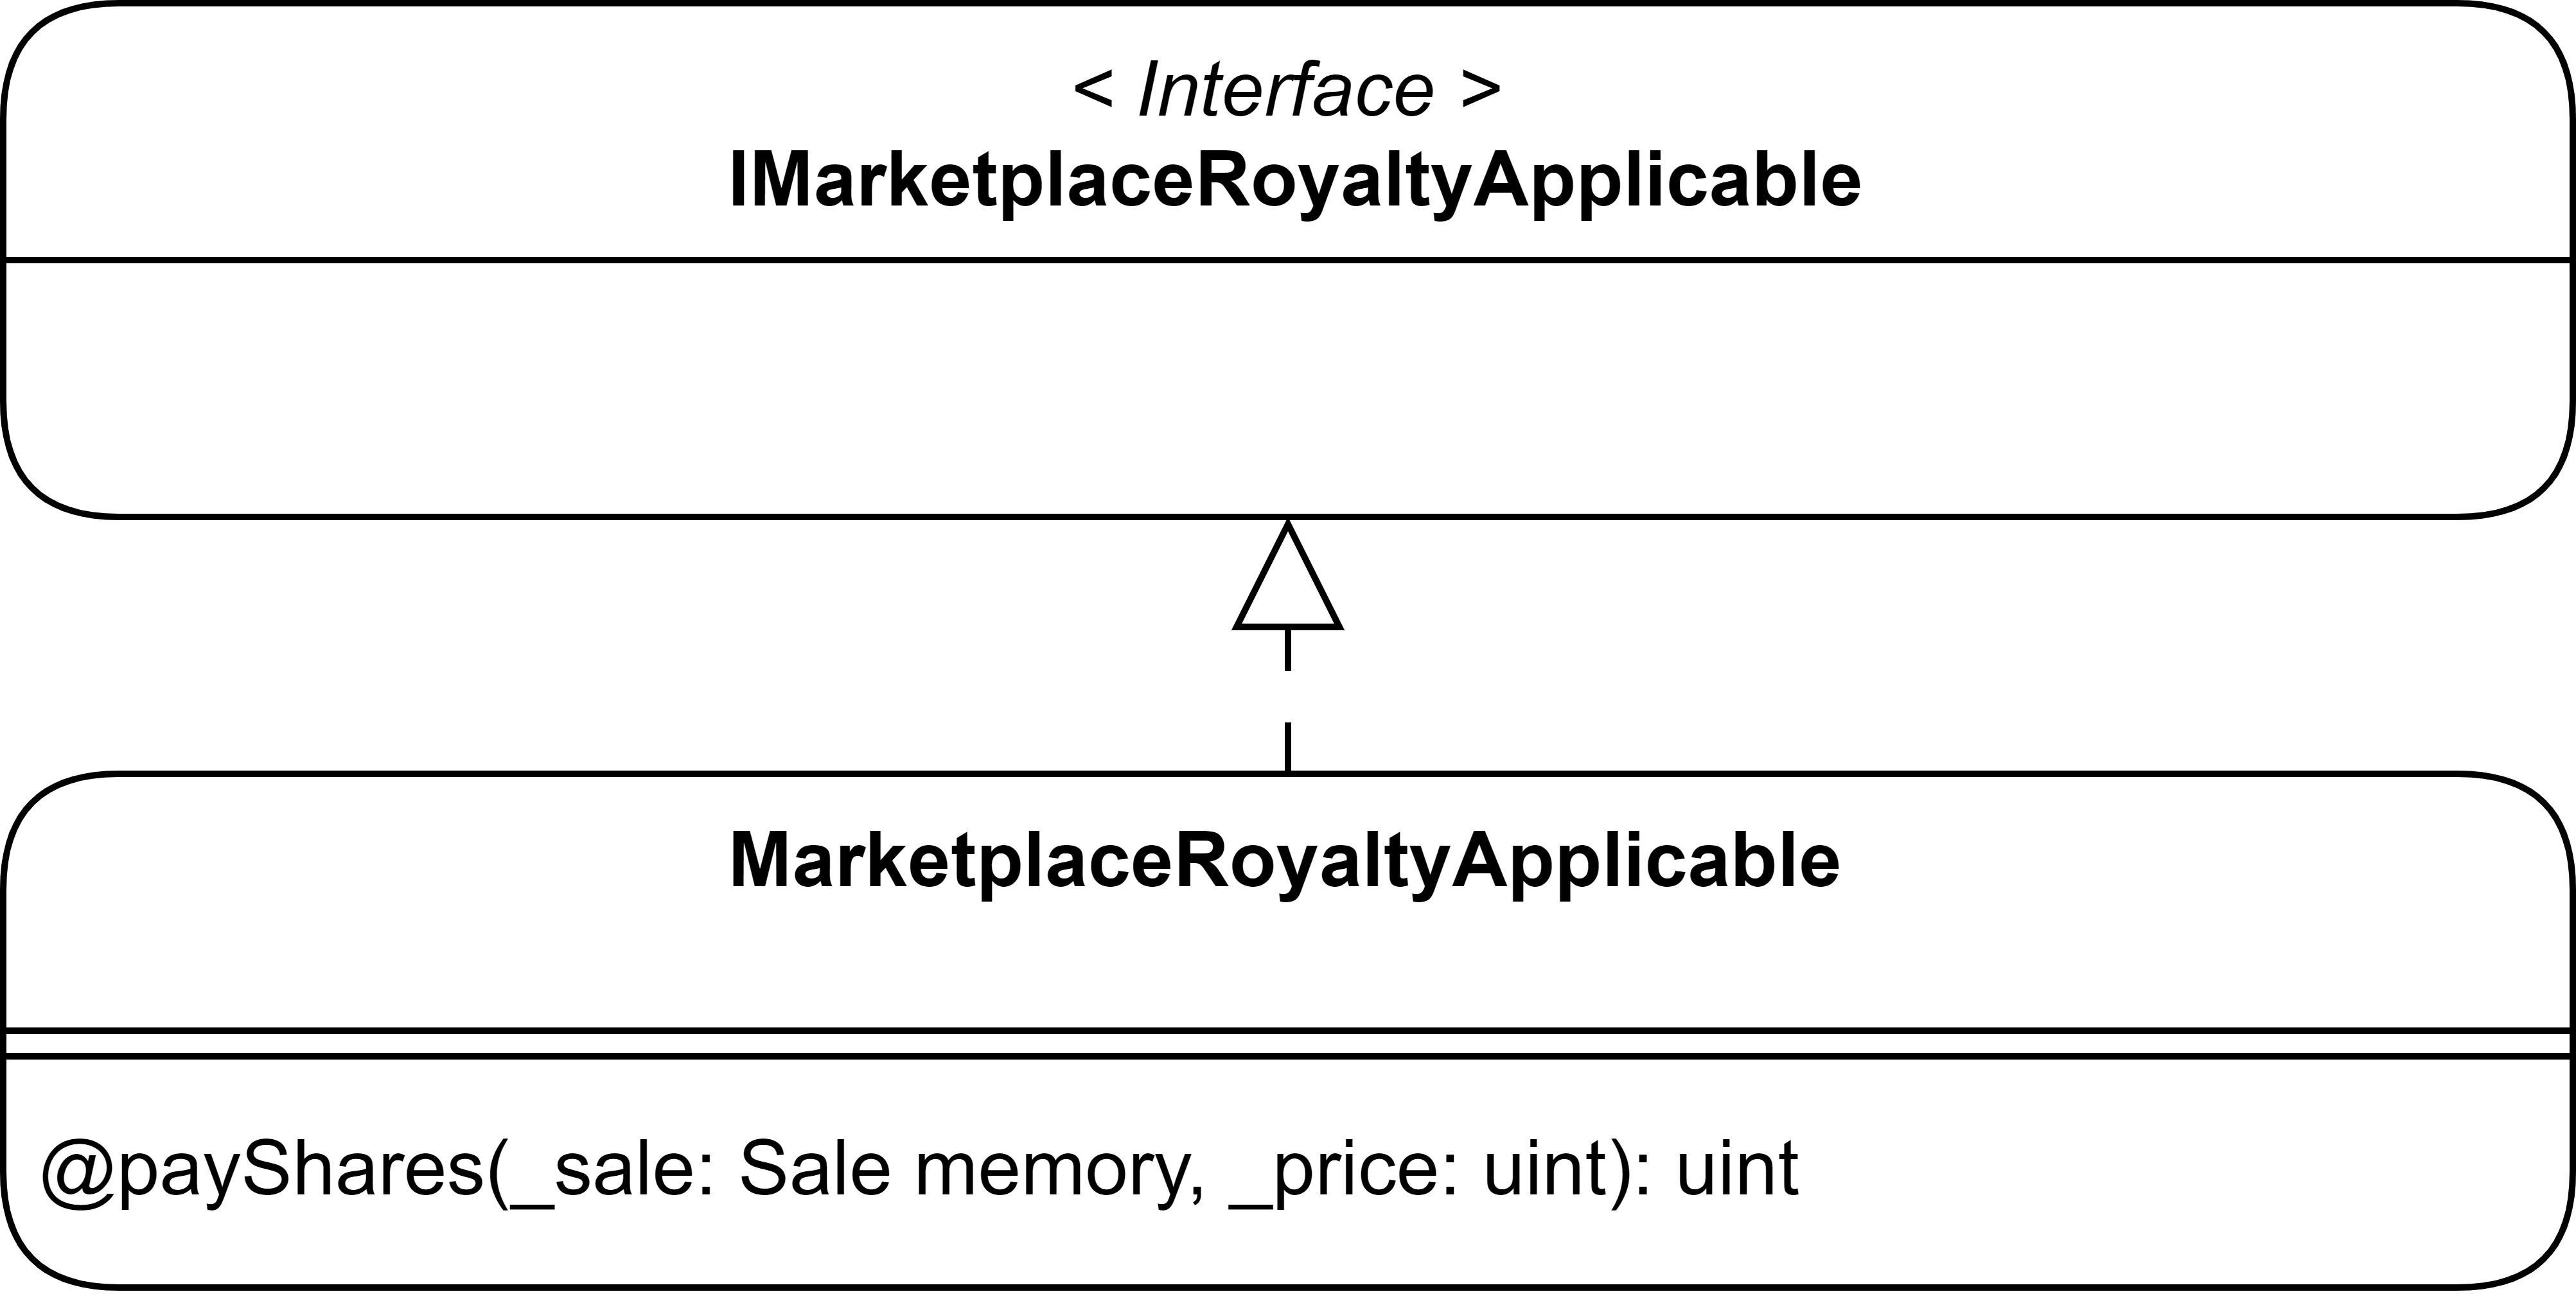
\includegraphics[width=0.7\textwidth]{images/blockchainContracts/MarketplaceRoyaltyApplicable.png}
    \caption{Marketplace RoyaltyApplicable}
    \label{fig:marketplaceRoyaltyApplicable}
\end{figure}


\paragraph{Cleanable}

All'interno del contratto \textit{Cleanable}, come rappresentato in figura \ref{fig:marketplaceCleanable}, sono presenti due metodi di gestione utilizzabili unicamente dall'amministratore, le loro funzionalità sono le seguenti:

\begin{itemize}
    \item \textit{cleanStorage}: Le informazioni relative a vendite cancellate o vendute rimangono all'interno del contratto. \textit{cleanStorage} permette di eliminare le informazioni relative a queste vendite allo scopo di ridurre la quantità di dati salvati all'interno del contratto, permettendo la riduzione dei tempi di attesa per l'esecuzione di alcune funzionalità sia \textit{on-chain} che \textit{off-chain}. Durante la progettazione del contratto è stato deciso di non cancellare queste informazioni all'acquisto, così da permettere agli utenti di risparmiare sulle \textit{gas fee}.
    \item \textit{cleanInqualities}: Questo metodo permette di eliminare le informazioni relative a vendite che non sono più corrette. Tale situazione può accadere nel momento in cui un utente trasferisce un asset in vendita esternamente al marketplace. In questo caso, la vendita rimarrebbe presente nel marketplace ma non sarebbe più valida. Un'alternativa per risolvere il problema è descritta nel capitolo \hyperref[sec:marketplace-royalty-applicable]{\textit{RoyaltyApplicable}}.
\end{itemize}

\begin{figure}[H]
    \centering
    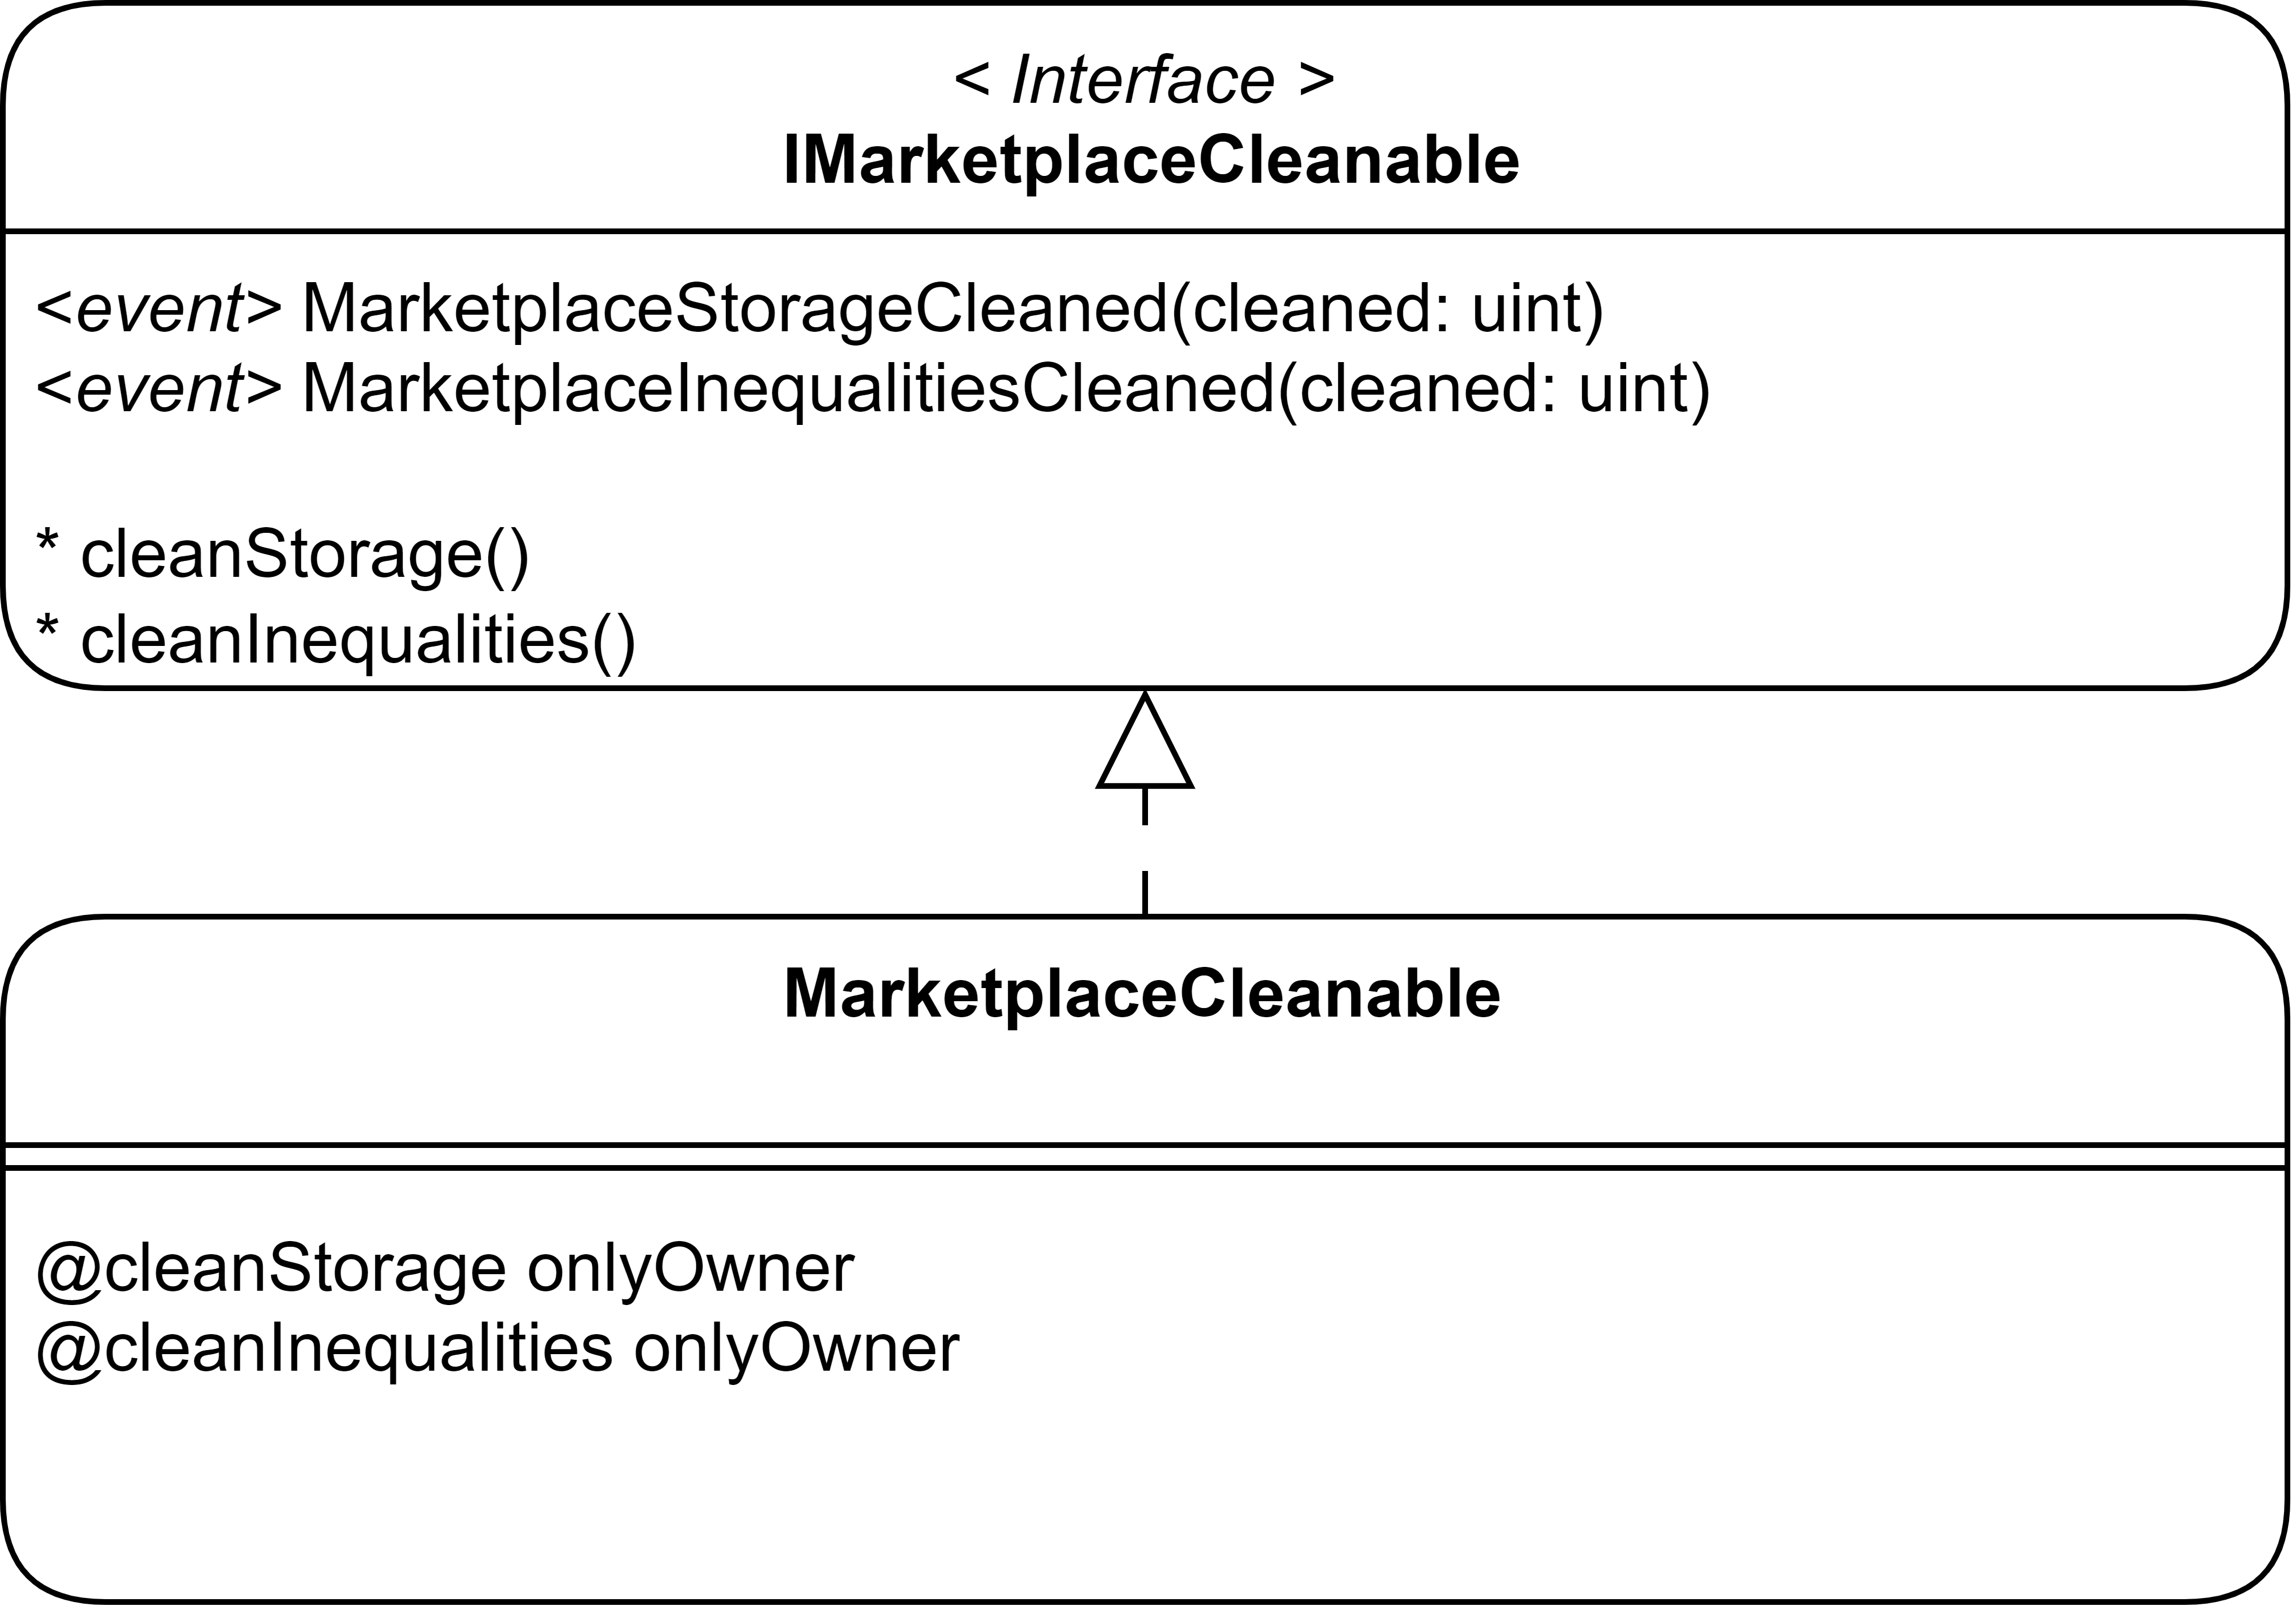
\includegraphics[width=0.7\textwidth]{images/blockchainContracts/MarketplaceCleanable.png}
    \caption{Marketplace Cleanable}
    \label{fig:marketplaceCleanable}
\end{figure}


\subsubsection{ERC721 Factory}

Come descritto nel capitolo \hyperref[sec:creazioneNFT]{\textit{Creazione NFT}}, l'utente ha tre possibilità per la generazione di un NFT, tra cui la creazione di una nuova collezione attraverso il \textit{depolyment} di un contratto ERC721. Per facilitare l'ultima operazione descritta, è stato sviluppato lo \textit{smart contract} \textit{ERC721 Factory}. Il quale permette di creare nuovi contratti utilizzando un \textit{template} chiamato \textit{Boilerplate ERC721}, analizzato nel prossimo capitolo. Come è possibile notare dalla figura \ref{fig:erc721Factory} il contratto presenta due metodi:

\begin{itemize}
    \item \textit{createERC721}: permette la creazione di un nuovo contratto ERC721, impostando un base URI per i metadati dei token (l'URI completo sarà composto da base URI + token ID), il nome e il simbolo della collezione. Inoltre, il metodo permette di impostare le \textit{royalties} di default per l'intero contratto e di effettuare l'operazione di \textit{mint} per un numero definito di asset.
    \item \textit{getAllERC721s}: questo metodo consente di ottenere tutti i contratti ERC721 creati attraverso la \textit{factory}. La sua utilità si presenta nel momento in cui l'utente vuole creare un nuovo NFT all'interno di una collezione già esistente. Infatti, filtrando in base all'\textit{owner} tutti i contratti ERC721, sarà possibile fornire all'utente unicamente quelli su cui ha il permesso di creare un nuovo NFT.
\end{itemize}

\begin{figure}[H]
    \centering
    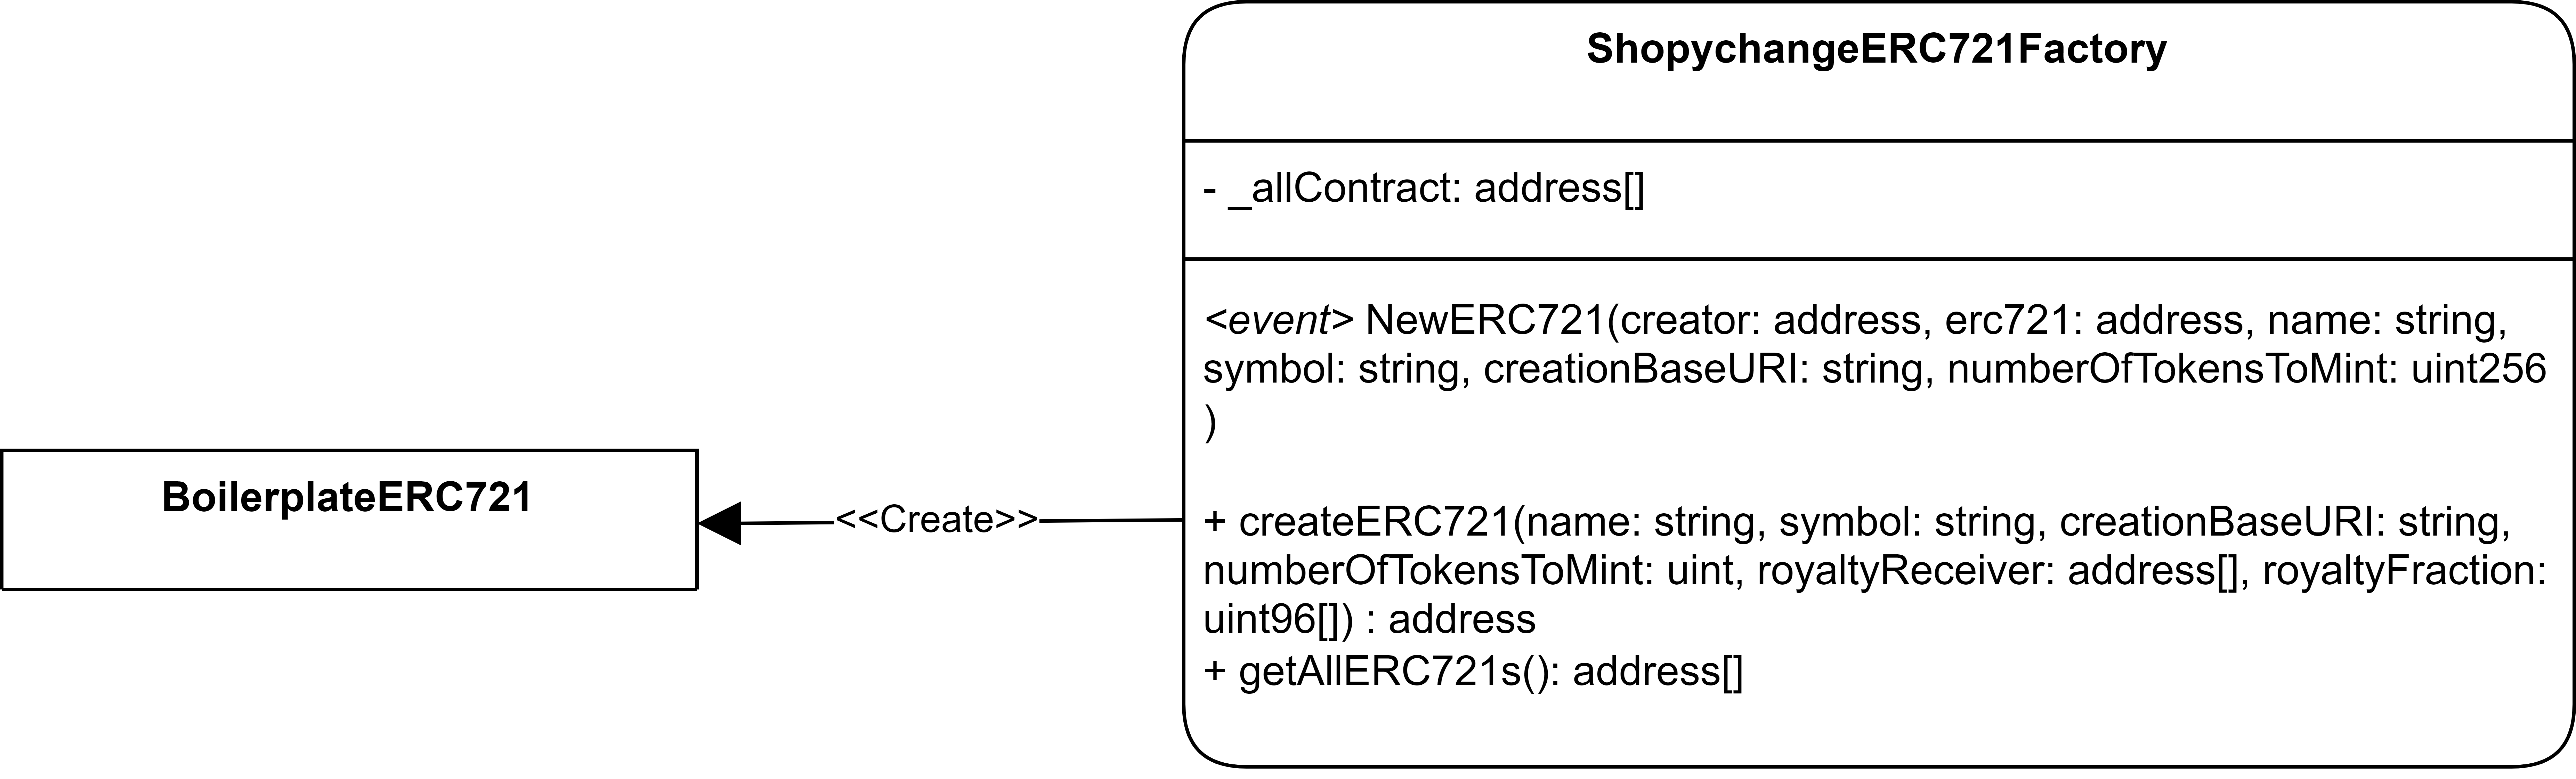
\includegraphics[width=0.7\textwidth]{images/blockchainContracts/ERC721Factory.png}
    \caption{ERC721 Factory}
    \label{fig:erc721Factory}
\end{figure}


\subsubsection{Boilerplate ERC721}

Il contratto \textit{Boilerplate ERC721} è un \textit{template} utilizzato per la creazione di nuovi contratti ERC721. Come visibile in figura \ref{fig:boilerplateERC721}, il contratto eredita da \textit{ERC721URIStorage}, \textit{ERC721Burnable} e \textit{ERC2981MultiReceiver}, questo permette di avere dei metadati per ogni token, di poter bruciare un token e di poter gestire le \textit{royalty} in maniera personalizzata.

\begin{figure}[H]
    \centering
    \includegraphics[width=0.7\textwidth]{images/blockchainContracts/BoilerplateERC721.png}
    \caption{BoilerplateERC721}
    \label{fig:boilerplateERC721}
\end{figure}

\paragraph{ERC2981MultiReceiver}
\label{sec:erc2981-multi-receiver}

Il contratto \textit{ERC2981MultiReceiver} è stato sviluppato per consentire la gestione delle \textit{royalty} in maniera personalizzata. 

Come visibile in figura \ref{fig:boilerplateERC721}, il contratto eredita da \textit{IERC2981Royalties}, il quale definisce le funzionalità obbligatorie per la gestione delle \textit{royalties}.

Come descritto più in dettaglio nel capitolo \hyperref[sec:utilizzo-erc2981-payment-splitter]{\textit{Utilizzo di ERC2981 e PaymentSplitter}} il contratto \textit{ERC2981MultiReceiver} è stato creato per poter gestire le \textit{royalties} con più di un ricevente. Infatti, già nel momento di creazione di un nuovo contratto \textit{BoilerplateERC721}, nel caso in cui vengano specificati più indirizzi, avverrà la creazione di un \textit{PaymentSplitter} di default. In questo modo, nel momento in cui avviene un acquisto, il saldo verrà diviso in base alla percentuale definita per ogni indirizzo. In aggiunta, il contratto permette la creazione di \textit{royalty} personalizzate per ogni token, creando contratti \textit{PaymentSplitter} all'occorenza.

\paragraph{PaymentSplitter}

Il contratto \textit{PaymentSplitter} offre la possibilità di dividere il saldo in base alla percentuale definita per ogni indirizzo. Nel momento in cui avviene un acquisto, il marketplace, o più specificamente il contratto \hyperref[sec:marketplace-royalty-applicable]{\textit{RoyaltyApplicable}}, invierà il saldo relativo alle \textit{royalties} al contratto \textit{PaymentSplitter}. Tuttavia, a causa di una limitazione implementativa del metodo \textit{receiver}, sarà compito dei riceventi di recupare il saldo ottenuto, l'operazione è possibile tramite il metodo \textit{release}. All'interno del capitolo \hyperref[sec:revenue-share]{\textit{Revenue Share}} è possibile osservare un esempio di utilizzo del contratto \textit{PaymentSplitter}.

\subsubsection{Storage}
Il contratto storage è semplicemente un contratto \textit{BoilerplateERC721} con la particolarità che chiunque può effettuare l'operazione di \textit{mint}. Esso è stato sviluppato per permettere a tutti glii utenti di creare un singolo asset senza la necessità di creare una collezione. 

\subsection{Scripts}

Per le operazioni di distribuzione dei contratti sono stati creati degli script appositi, i quali permettono l'automazione di alcuni processi ripetitivi.

Lo script chiamato \textit{copyArtifacts} permette di copiare gli artefatti generati dalla compilazione degli smart contracts in una cartella definita.

Lo script \textit{modifyEnv} ha lo scopo di modificare i file \textit{.env}, ovvero i file di configurazione presenti sia nel frontend che nel backend. Più in dettaglio, questo script permette di modificare il valore di variabili definite con uno nuovo. Il suo utilizzo è molto utile nel momento in cui si effettua il \textit{deploy} di un contratto. Infatti, il contratto appena distribuito avrà un indirizzo diverso rispetto a quello precedente ed è quindi necessario modificare i file di \textit{envirorment} per permettere al frontend e al backend di interagire con il nuovo contratto.

Infine, è stato creato uno script chiamato \textit{deployAll}, esso permette di distrubito tutti i contratti sopracitati aggiornando gli artefatti e modificando i file \textit{.env}.

\subsection{Test}

Per verificare il corretto funzionamento degli smart contracts sono stati sviluppati dei test utilizzando la libreria \textit{ethers}, già presente nel framework \textit{Hardhat}. I test effettuati sono di due tipi: \textit{unit test} e \textit{integration test}.
I primi si occupano di verificare il corretto funzionamento di una singola funzionalità all'interno di un contratto. Mentre i secondi, si occupano di verificare il corretto funzionamento di più funzionalità all'interno di più contratti oppure di un singolo contratto generato ereditando più moduli, come nel caso del contratto \textit{ShopychangeMarketplace}.

\subsection{Motivazioni e Alternative}

La scelta che ha portato all'utilizzo di \textit{Hardhat} è stata fatta in quanto è un framework molto utilizzato e ben documentato, inoltre permette di creare un'istanza di un nodo locale, così da poter utilizzare una blockchain locale rendendo più semplice lo sviluppo e i test dell'intera applicazione. Per quanto riguarda la scelta del linguaggio di programmazione, è stato deciso di utilizzare \textit{Solidity} in quanto è il linguaggio più utilizzato per lo sviluppo di smart contracts. Inoltre, è possibile trovare una vasta documentazione e numerosi esempi di codice. 

In aggiunta, Durante lo svolgimento del progetto è stato utilizzato anche il webtool \textit{Remix}, il quale permette di scrivere, compilare e distribuire gli \textit{smart contracts}. In aggiunta, \textit{Remix} ha la funzionalità di poter interagire con gli \textit{smart contracts} attraverso dei semplici pulsanti, velocizzando l'interazione.

Inoltre, durante la fase di sviluppo è stato deciso di non utilizzare \textit{Typechain}, il quale permette di generare dei tipi TypeScript a partire dagli smart contracts. Questa scelta è stata fatta in quanto la libreria di interazione con i contratti a livello frontend (\textit{wagmi}) non supporta i tipi generati da \textit{Typechain}. Tuttavia, è possibile utilizzare \textit{Typechain} in combinazione con \textit{ethers} (una libreria largamente utilizzata per l'interazione con gli smart contracts).

Le alternative in ambito implementativo sono molteplici, così come le tecnologie utilizzabili. In particolare, per lo sviluppo degli smart contracts è possibile utilizzare diversi linguaggi di programmazione, tra cui \textit{Solidity}, \textit{Vyper} e \textit{Fe}. Anche i framework utilizzabili sono numerosi, tra cui \textit{Hardhat}, \textit{Truffle}\footnote{https://trufflesuite.com/} e \textit{Embark}\footnote{https://framework.embarklabs.io/}.

\newpage

\section{Backend}
\label{sec:backend}

Nel capitolo seguente verrà descritto in maniera più approfondita il modulo \textit{backend}, ovvero il modulo che si occupa di gestire le richieste provenienti dal \textit{frontend} filtrando i dati presenti nella blockchain e nel database. Il modulo è stato sviluppato utilizzando il linguaggio di programmazione \textit{python} ed il framework \textit{Django}. 

È importante sottolineare che sebbene avere un server di \textit{backend} possa sembrare in contrasto con il principio di decentralizzazione, la sua presenza è fondamentale per ottimizzare i tempi di risposta e fornire agli utenti un'esperienza d'uso migliore.  Inoltre, come si potrà notare nel capitolo, il \textit{backend} ha il solo scopo di essere da tramite e filtro tra il \textit{frontend} e la blockchain.

\subsection{API}

Lo scopo principale del modulo \textit{backend} è quello di fornire delle \textit{Application programming interface} (API) al \textit{frontend} con i dati necessari per la visualizzazione delle informazioni. In particolare, le API devono permettere di recuperare le informazioni relative ad un asset, ad una collezione e ad un utente. Inoltre, devono permettere di recuperare le informazioni relative alle vendite in corso presenti sul marketplace. Per offrire le funzionalità appena descritte, è stato deciso di utilizzare \textit{GraphQL}\footnote{https://graphql.org/}, un linguaggio di \textit{query} API alternativo a \textit{REST}.

Di seguito è possibile vedere un esempio di \textit{query} GraphQL per recuperare le informazioni degli asset posseduti da un utente. Si noti come sia possibile specificare quali informazioni si vogliono ricevere in risposta, in questo caso il nome, l'indirizzo del contratto e l'identificativo dell'asset. Seppure nell'API progettata sia possibile richiedere anche altre informazioni come l'immagine e i metadati.

\begin{lstlisting}[basicstyle=\small]
    query {
        ownedNfts(address: "0x...") {
            contractAddress
            tokenId
            name
        }
    }
\end{lstlisting}

Il framework \textit{Django} permette la creazione di \textit{app}, ovvero moduli interni che consentono una maggiore modularità e organizzazione del codice. Quando configurato con \textit{GraphQL}, ogni \textit{app} genera automaticamente uno \textit{schema}, ossia un insieme di \textit{query} e \textit{mutation}. Le \textit{query} sono funzioni che permettono di recuperare i dati, mentre le \textit{mutation} permettono di modificarli. In particolare, le \textit{mutation} sono utilizzate per interagire con il database.

Con la configurazione di base di \textit{Graphene}\footnote{https://graphene-python.org/} (libreria con lo scopo di semplificare l'integrazione di \textit{GraphQL}), ogni \textit{app} genera un proprio URI nel quale è possibile effettuare le richieste. 

Per semplificare l'implementazione e l'interazione con le API è stato deciso di implementare il concetto di \textit{Federation schema}. Esso permette di creare uno schema unico che contiene tutte le \textit{query} e le \textit{mutation} disponibili, mantenendo comunque la modularità del codice. In questo modo, è possibile effettuare una singola richiesta per recuperare i dati da più \textit{app} differenti.

Entrando più nel dettaglio nell'implementazione effettuata, il \textit{backend} è composto da tre \textit{app} differenti:

\begin{itemize}
    \item \textit{BlockchainAPI}: Si occupa di recuperare i dati dalla blockchain, specialmente i dati relativi a collezioni, asset ed eventi.
    \item \textit{MarketplaceAPI}: Recupera tutte le informazioni relative al marketplace.
    \item \textit{databaseAPI}: Interagisce con il database, in particolare con i dati relativi all'utente.
\end{itemize}

La figura \ref{fig:federationSchema} rappresenta lo schema delle API, in particolare è possibile notare il funzionamento del \textit{Federation schema} e del modulo \textit{backend}.

\begin{figure}[H]
    \centering
    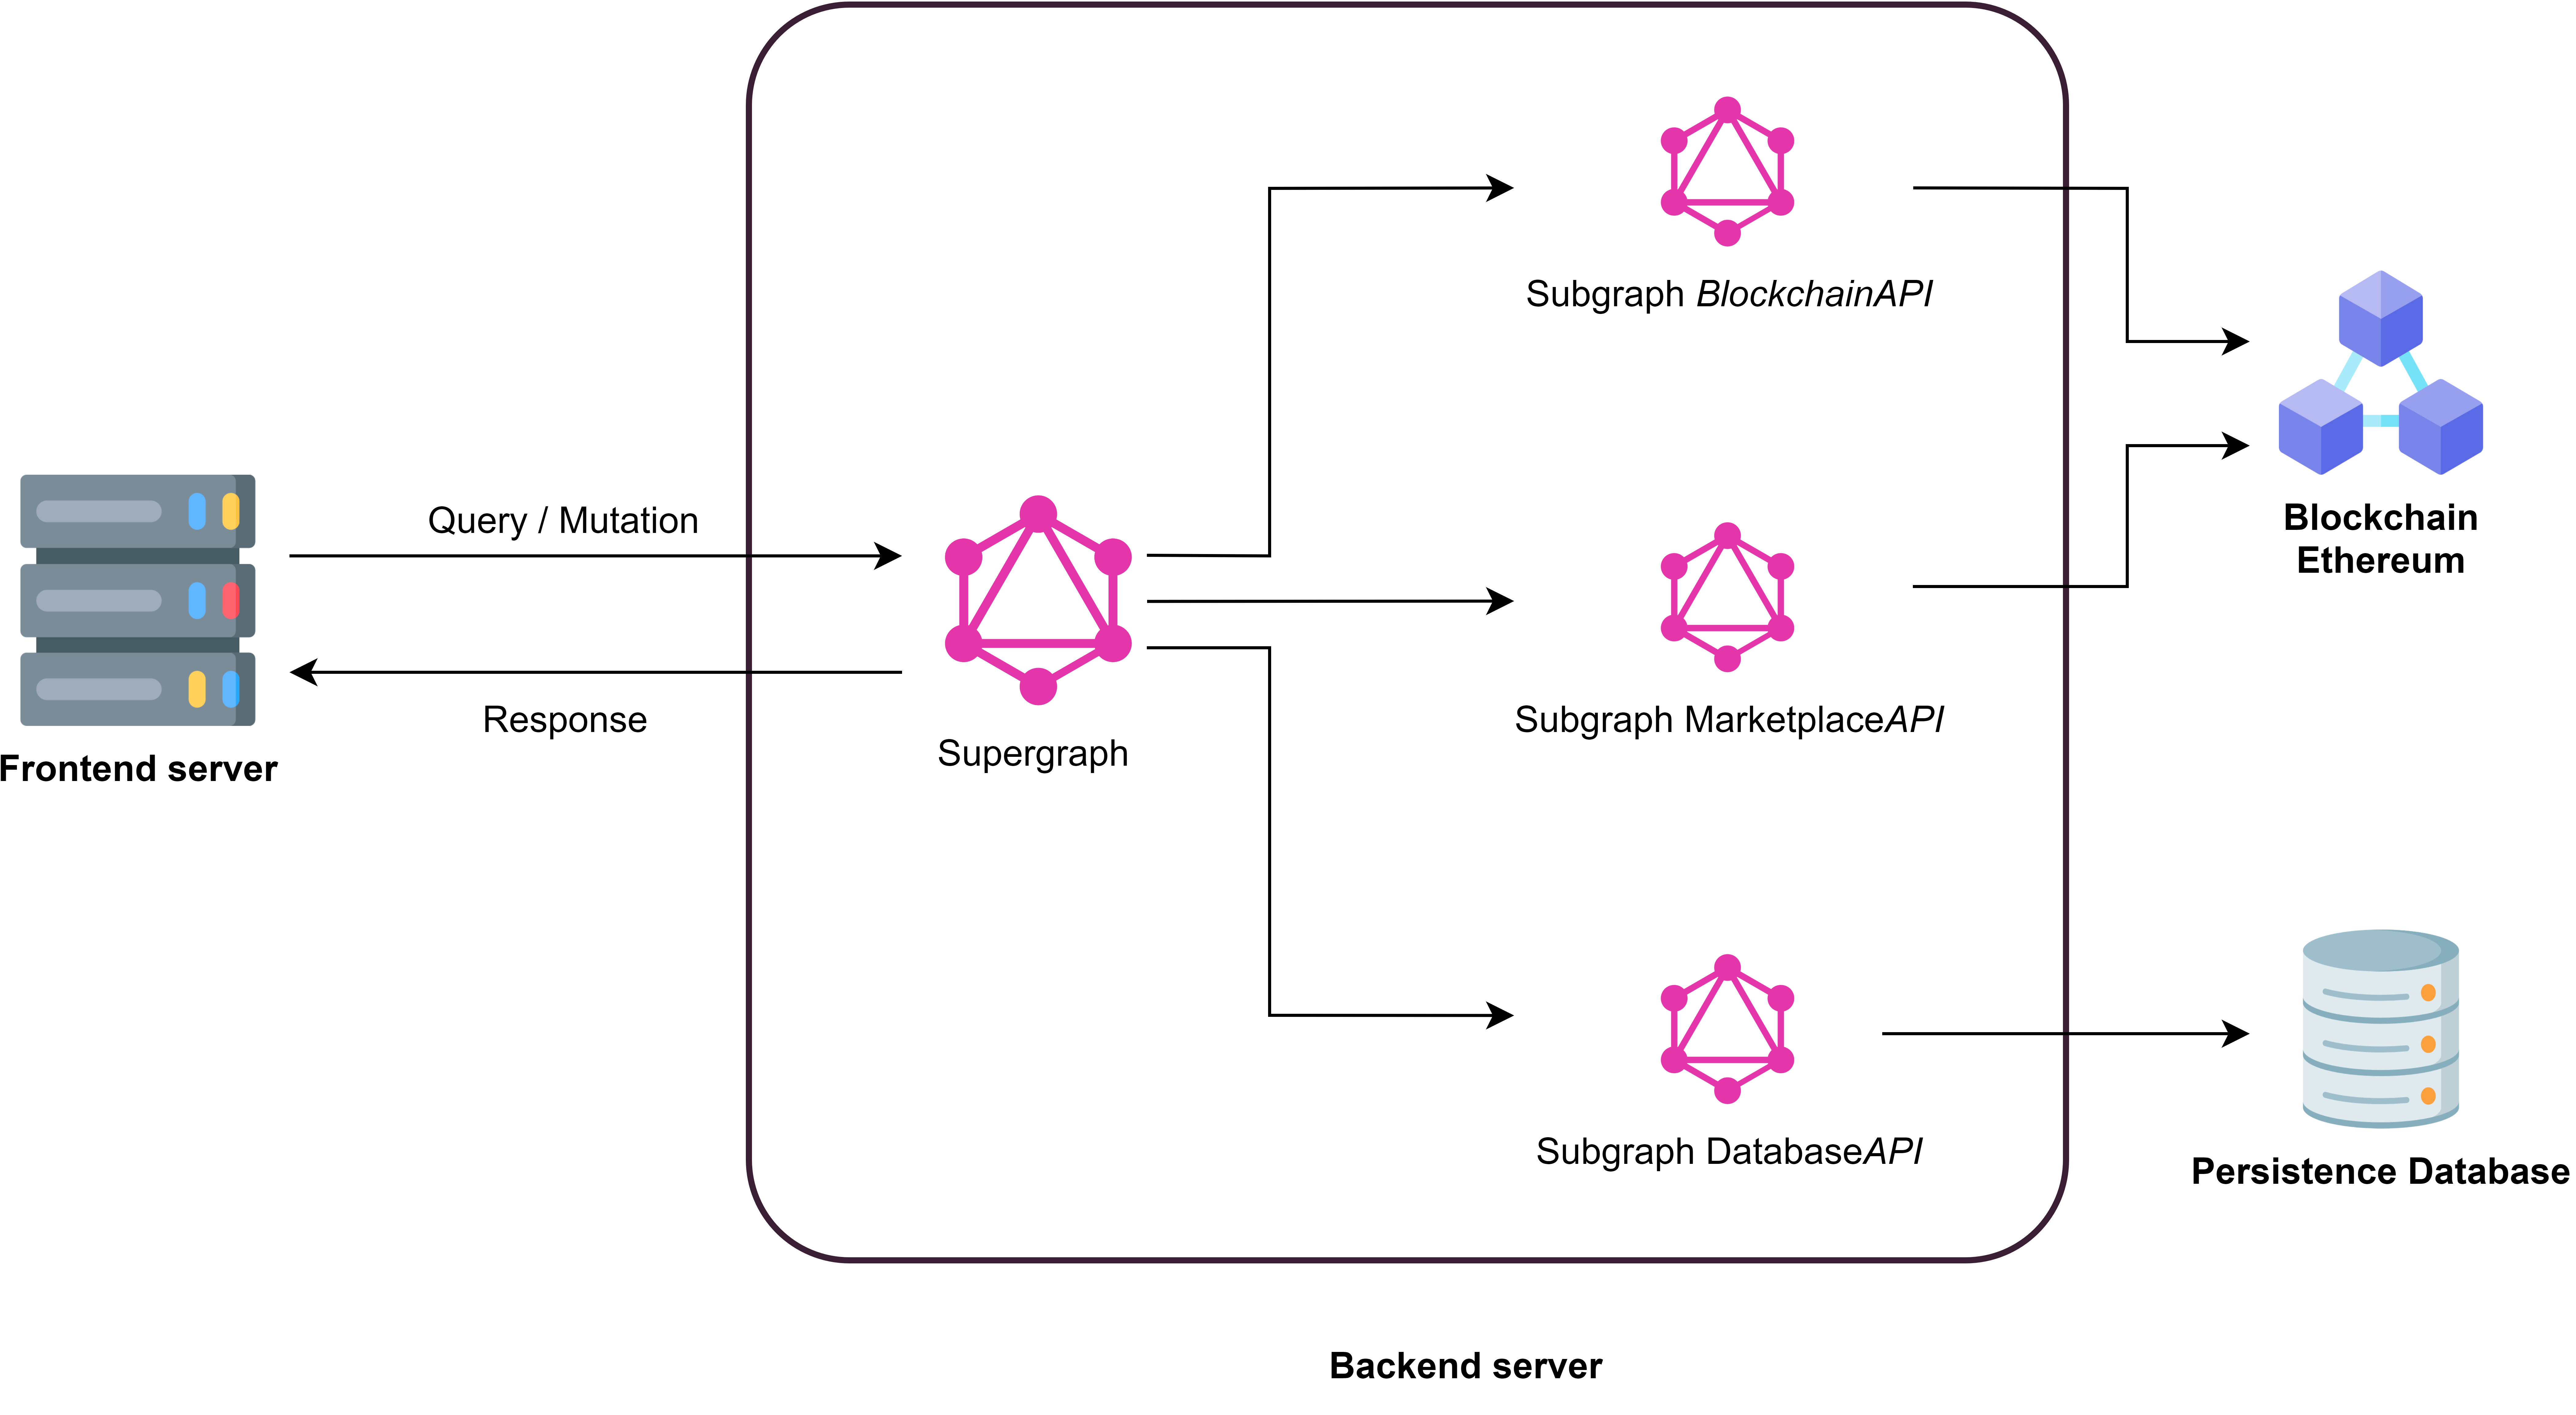
\includegraphics[width=1\textwidth]{images/GraphQLFederationSchema.png}
    \caption{Schema delle API}
    \label{fig:federationSchema}
\end{figure}

All'interno dei prossimi capitoli verranno analizzate le \textit{query} e le \textit{mutation} disponibili nelle tre \textit{app}.

\subsubsection{Blockchain API}

All'interno del \textit{subgraph Blockchain API} sono presenti diverse query che permettono di recuperare le informazioni presenti nella blockchain. Come descritto nel capitolo \hyperref[sec:recuperoDatiBlockchain]{\textit{Recupero dei dati dalla blockchain}} è possibile recuperare i dati di una collezione solamente se si conosce l'indirizzo del contratto che la rappresenta.
Di seguito è presente una lista delle principali \textit{query} disponibili, con il relativo scopo e funzionamento.

\begin{itemize}
    \item \textit{ownedNfts}: Recupera tutti gli asset posseduti da un utente specifico. filtrando gli eventi \textit{Transfer} presenti negli smart contracts da lui osservati.
    \item \textit{nftComplete}: Recupera tutte le informazioni relative ad un asset, contattando lo smart contract e analizzando i metadati su IPFS.
    \item \textit{collection}: Ritorna le informazioni di una collezione e tutti gli asset presenti al suo interno, contattando lo smart contract e filtrando gli eventi di \textit{Transfer} in base alla tipologia (\textit{Mint} o \textit{Burn}).
    \item \textit{contract}: Risolve unicamente le informazioni base di un contratto. Ovvero il nome, il simbolo e l'indirizzo.
    \item \textit{nftHistory}: Analizzando gli eventi di trasferimento, approvazione e relativi al marketplace di un asset, ritorna la cronologia completa di un asset.
    \item \textit{royaltyCollection}: Contattando il contratto della collezione, recupera le informazioni riguardanti le royalty di default per una collezione, ritornando la compatibilità con lo standard ERC2981 e/o ERC2981MultiReceiver, nonchè la percentuale per ogni ricevente.
    \item \textit{withdrawRoyaltyCollection}: Nel caso in cui la collection possieda un PaymentSplitter, ritorna l'ammontare che è possibile prelevare.
    \item \textit{royaltyToken} e \textit{withdrawRoyaltyToken}: Come le \textit{query} precedenti, ma per un singolo asset.
    \item \textit{collectionOwner}: Verifica che l'indirizzo passato come parametro sia il proprietario di una collezione, anch'essa passata come parametro. Questa \textit{query} è utilizzata per verificare che l'utente abbia il diritto di accedere alla pagina di gestione di una collezione.
    \item \textit{contractOwnedCreatedWithShopychange}: Come descritto nel capitolo \hyperref[sec:creazioneNFT]{\textit{Creazione NFT}}, questa \textit{query} ritorna gli indirizzi di collezioni creati tramite Shopychange.
\end{itemize}

\subsubsection{Marketplace API}

L'\textit{app Marketplace API} si occupa di recuperare le informazioni relative al marketplace. All'interno dello schema sono presenti le seguenti \textit{query}:

\begin{itemize}
    \item  \textit{sales}: Recupera tutte le vendite in corso presenti sul marketplace, contattando il metodo all'interno del contratto \textit{MarketplaceFundamental}.
    \item \textit{sale}: Ottiene le informazioni di vendita di uno specifico token.
    \item \textit{isMarketplaceApproved}: Verifica che il marketplace sia approvato per la gestione di un asset.
    \item \textit{isTokenForSale}: Verifica che un asset sia in vendita.
    \item \textit{marketplaceRoyalty}: Recupera la percentuale di revenue share che il marketplace richiede per ogni vendita.
    \item \textit{marketplaceBalace}: Ottiene il bilancio del marketplace ottenuto tramite il revenue share.
\end{itemize}

\subsubsection{Database API}

Lo schema \textit{Database API} presenta le \textit{query} e \textit{mutation} per recuperare e modificare i dati presenti nel database. Più nel dettaglio, i dati modificabili sono una lista di collezioni che l'utente vuole monitorare. Le \textit{query} e \textit{mutation} sono le seguenti:

\begin{itemize}
    \item \textit{ContractObserved}: Ritorna la lista di collezioni che l'utente vuole monitorare.
    \item \textit{AddUser}: Aggiunge un utente al database.
    \item \textit{AddNFTCollection}: Aggiunge una collezione alla lista di collezioni monitorate da un utente.
    \item \textit{AddNFTCollections}: Come la \textit{mutation} precedente, ma per più collezioni.
    \item \textit{RemoveNFTCollection}: Rimuove una collezione dalla lista di collezioni osservate da un utente.
    \item \textit{RemoveNFTCollections}: Come la \textit{mutation} precedente, ma per più collezioni.
\end{itemize}

\subsection{Database}

Il database è stato implementato utilizzando \textit{MongoDB}, un database non relazionale che permette di salvare i dati su documenti. Il database è stato collegato utilizzando la libreria \textit{djongo}\footnote{https://www.djongomapper.com/} che permette di connettere \textit{Django} con \textit{MongoDB}. Essendo che il progetto sviluppato è una \textit{dApp}, le informazioni da salvare sono poche e non fondamentali per il funzionamento del sistema. Infatti, l'unica informazione salvata sul database è la lista di collezioni che l'utente ha deciso di osservare. In aggiunta, è presente una tabella che contiene una lista di collezioni generiche che tutti gli utenti monitorano, l'obiettivo è di permettere agli utenti di visualizzare le collezioni più popolari senza doverle cercare manualmente.

\subsection{Test}

Tutte le query e mutation presenti nel \textit{Federation schema} sono completamente testate utilizzando il \textit{tool} già integrato in \textit{Django}. I test verificano che i dati vengano filtrati, elaborati e restituiti correttamente sia in caso di parametri validi che non validi. Inoltre, sono stati implementati dei test per verificare la giusta gestione degli errori in caso di valori non previsti restituiti dalla blockchain e dal database.

\subsection{Motivazioni e Alternative}

Le alternative a livello di linguaggio di programmazione e framework sono molteplici, la sceltà è però da ricondurre alle librerie di connessione con la blockchain in quanto sono meno numerose. Di queste, le più famose e utilizzate sono:

\begin{itemize}
    \item \textit{Web3.js}\footnote{https://web3js.readthedocs.io/}: Libreria JavaScript/TypesScript
    \item \textit{Web3.py}\footnote{https://web3py.readthedocs.io/}: Libreria Python
    \item \textit{Ethers.js}\footnote{https://docs.ethers.org/v5/}: Libreria JavaScript/TypesScript
\end{itemize}

Essendo il \textit{frontend} sviluppato utilizzando \textit{Typescript}, come definito dai requisiti del progetto. La scelta è ricaduta su \textit{Web3.py} così da ampliare le conoscenze e competenze in ambito di sviluppo Python. 

Pertanto, avendo conoscenze ridotte nell'ambito Python è stato deciso di utilizzare il framework \textit{Django}, in quanto è uno dei più utilizzati e ricco di documentazione. Una possibile alternativa è \textit{Flask}\footnote{https://flask.palletsprojects.com/}.

La decisione che ha portato all'adozione di API di tipo GraphQL, quindi non API di tipo REST, è stata presa in quanto offrono maggiore flessibilità ed efficienza. Più in dettaglio, tramite il linguaggio \textit{query} utilizzato da GraphQL è possibile richiedere informazioni da più \textit{app}/\textit{endopoint} in una singola richiesta. Inoltre, GraphQL permette di definire quali informazioni si vogliono ricevere in risposta, in questo modo è possibile ridurre il traffico di rete e il tempo di risposta ma senza dover implementare nuove \textit{query}.

Infine, GraphQL presenta un sistema di \textit{cache} che permette di ridurre ulteriormente il tempo di risposta, in quanto è possibile salvare in cache le risposte alle richieste più frequenti. Tuttavia, quest'ultima funzionalità è stata disabilitata così da ottenere sempre le informazioni dalla blockchain più aggiornate ed evitare problemi di inconsistenza dei dati.

\section{Frontend}

All'interno di questa sezione verrà descritto il modulo \textit{Frontend}, il quale si occupa di gestire l'interfaccia grafica dell'applicazione richiedendo le informazioni necessarie al modulo \textit{Backend} e creando richieste agli smart contracts visti nel capitolo \hyperref[sec:blockchain-module]{\textit{Blockchain}}.
Il framework utilizzato per lo sviluppo è \textit{React}, il quale permette di creare applicazioni web responsive e dinamiche. In aggiunta, è stato deciso di utilizzare il linguaggio \textit{TypeScript} per lo sviluppo del modulo, in quanto permette di definire tipi statici per le variabili e di conseguenza di ridurre gli errori di programmazione.

\subsection{Librerie}

Per il corretto funzionamento del modulo sono state scelte alcune librerie di fondamentale importanza. Di seguito verranno elencate e descritte le principali.

\begin{itemize}
    \item \textit{WalletConnect}\footnote{https://walletconnect.com/}: libreria che permette di connettersi ad un wallet di diverso tipo (Web extension, Mobile, Desktop) e di conseguenza di interagire con la blockchain.
    \item \textit{Wagmi}\footnote{https://wagmi.sh/}: Consigliata da \textit{WalletConnect} per compatibilità, permette di creare transazioni e ottenere informazioni in Ethereum.
    \item \textit{ChakraUI}\footnote{https://chakra-ui.com/}: libreria grafica semplice e con una vasta gamma di componenti.
    \item \textit{React Router}\footnote{https://reactrouter.com/}: libreria che permette di gestire il routing all'interno di un'applicazione React. Con possibilità di creare una
    \textit{Single Page Application}.
\end{itemize}

\subsection{Struttura}
\label{sec:frontend-structure}

Sebbene React stesso non consigli una struttura file specifica \cite{react-structure}, è fondamentale organizzare il codice in modo da rendere la lettura e la manutenzione più semplice. Perciò, è stato deciso di dividere il codice seguendo questo schema:

\begin{lstlisting}[basicstyle=\small]
    src/
        assets/
            Imagini
        components/
            Ogni componente in una cartella separata
        pages/
            Ogni pagina in una cartella separata
        hooks/
            Hooks personalizzati
        context/
            Context providers
        utils/
            Funzioni di utility, ognuna in una cartella separata
        styles/
            Stile globale
        services/
            Servizi di comunicazione con il backend e blockchain
\end{lstlisting}

Inoltre, internamente alle cartelle \textit{assets}, \textit{components}, \textit{pages}, i file sono organizzati nel seguente modo:

\begin{lstlisting}[basicstyle=\small]
    NFTCard/
        __mocks__/
            NFTCard.tsx
        __tests__/
            __snapshots__/ # autogenerato
                NFTCard.test.tsx.snap 
          NFTCard.tsx
          useNFTCard.tsx
        NFTCard.tsx
        useNFTCard.tsx
\end{lstlisting}

L'esempio soprastante mostra la struttura del componente \textit{NFTCard}. All'interno della sua cartella sono presenti i file \textit{NFTCard.tsx} e \textit{useNFTCard.tsx}, i quali contengono rispettivamente il componente grafico ed il suo hook personalizzato. Questo approccio permette un ottimo livello di \textit{Separation of Concerns} e di conseguenza una maggiore manutenibilità del codice. Proseguendo, all'interno della cartella \textit{\_\_tests\_\_} sono presenti i file di test per il componente e per il suo \textit{hook}. Nel caso in cui sia necessario effettuare dei test sulla parte grafica, \textit{jest} genera automaticamente uno \textit{snapshot} del componente, il quale viene utilizzato per verificare che non ci siano cambiamenti involontari. Infine, all'interno della cartella \textit{\_\_mocks\_\_} è presente il file \textit{NFTCard.tsx} che viene utilizzato per simulare il componente durante i test in altri componenti.

\subsection{Componenti ricorrenti}

Nella cartella \textit{components} sono presenti i componenti che vengono utilizzati più volte all'interno delle pagine dell'applicazione. Di seguito una breve descrizione di ciascun componente.

\begin{itemize}
    \item \textit{PageLayout}: Gestisce il layout della pagina includendo l'header e il footer.
    \item \textit{AccountPopover}: Mostra le possibili azioni che l'utente può effettuare sul proprio account.
    \item \textit{NFTHistoryTable}: Mostra la cronologia delle transazioni effettuate sull'NFT.
    \item \textit{NFTCard}: Card per la visualizzazione di un NFT.
    \item \textit{NFTCardGrid}: Griglia di NFTCard.
    \item \textit{CollectionGrid}: Griglia di NFTCard organizzate per collezione.
    \item \textit{NFTORCollectionViewer}: Permette il cambio di visualizzazione tra NFTCardGrid e CollectionGrid.
    \item \textit{Buy}: Bottone per l'acquisto di un NFT comprensivo di modale per la conferma dell'acquisto.
    \item \textit{ModifySale}: Bottone per la modifica di un NFT in vendita comprensivo di modale per la conferma della modifica.
    \item \textit{CancelSale}: Bottone per la rimozione di un NFT dalla vendita comprensivo di modale per la conferma della rimozione.
    \item \textit{Sell}: Bottone per la messa in vendita di un NFT comprensivo di modale per la conferma della messa in vendita.
    \item \textit{NFTOperations}: Permette di visualizzare i bottoni di Buy, ModifySale, CancelSale, Sell in base allo stato dell'NFT e all'utente connesso.
    \item \textit{PriceDisibution}: Fornisce una visualizzazione grafica della distribuzione del prezzo di vendita di un NFT.
    \item \textit{Error}: Mostra un messaggio di errore.
    \item \textit{LoadingButton}: Bottone con un indicatore di caricamento.
    \item \textit{LoadingSpinner}: Indicatore di caricamento.
    \item \textit{ShadowButton}: Bottone standard dell'applicazione.
    \item \textit{UploadImage}: Gestisce il caricamento, cancellazione e visualizzazione di un'immagine.
    \item \textit{WithdrawRoyaltyButton}: Bottone per il ritiro delle royalty.
\end{itemize}

\subsection{Pagine}
Nel seguente capitolo verranno visualizzate e descritte le pagine dell'applicazione. Ogni pagina presenta la possibilità di cambiare tema tra \textit{light} e \textit{dark} ed è completamente \textit{responsive}, adattandosi a qualsiasi dispositivo. Essendo l'applicativo sviluppato dinamico e reattivo saranno discusse unicamente le pagine in fase iniziale e non quelle in seguito a delle azioni dell'utente. Inoltre, per ogni pagina verrà mostrata la versione desktop e mobile.

\subsubsection{Home}

La pagina \textit{Home} è la prima pagina che viene visualizzata all'apertura del sito. Il suo scopo è quello di mostrare gli NFT che sono attualmente in vendita. Nel caso in cui il wallet non sia collegato sarà visualizzato un messaggio che invita l'utente a collegarlo, altrimenti apparirà come in figura \ref{fig:home}.

\begin{figure}[H]
    \begin{minipage}{0.7\textwidth}
      \centering
      \fcolorbox{mint-cream}{white}{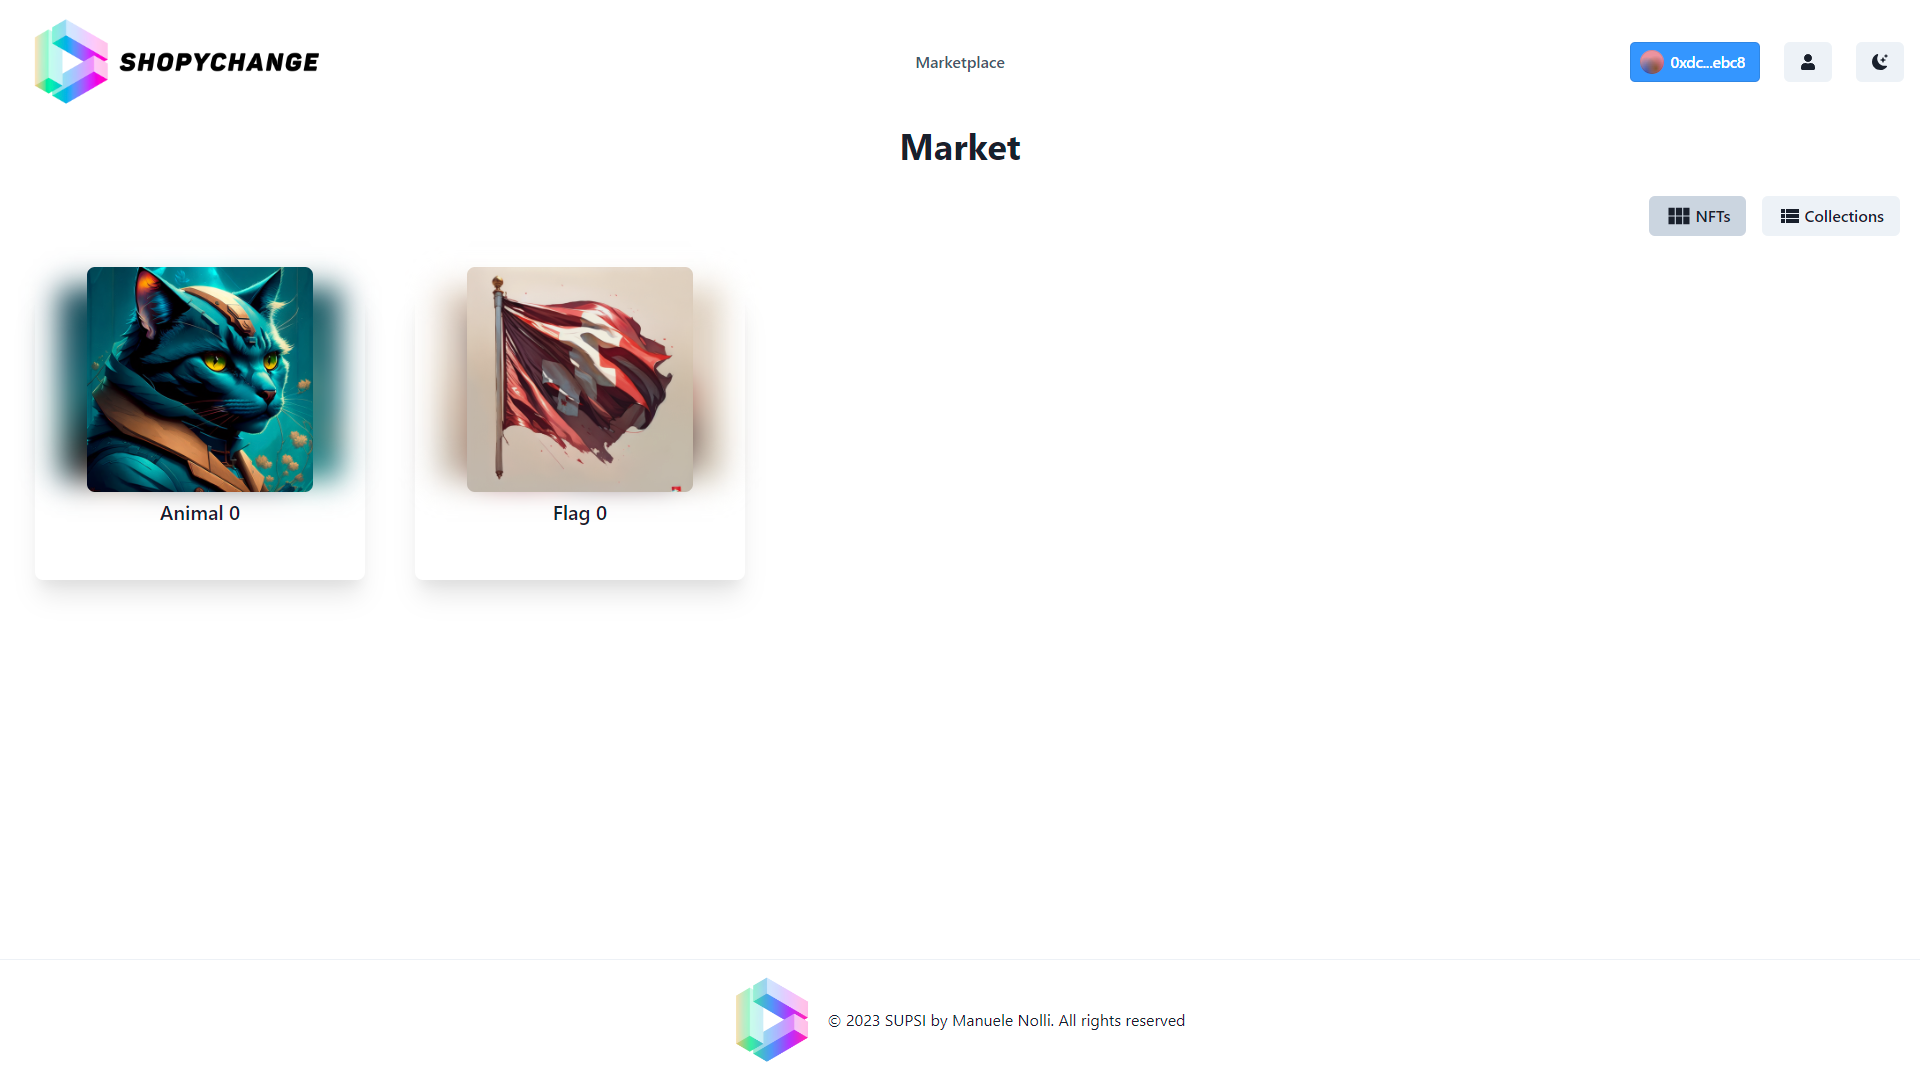
\includegraphics[width=\textwidth]{images/pages/home_connected.png}}
    \end{minipage}
    \hfill
    \begin{minipage}{0.26\textwidth }
      \centering
      \fcolorbox{mint-cream}{white}{
\includegraphics[width=\textwidth]{images/pages/home_connected_mobile.png}}
      \end{minipage}
      \caption{Pagina Home}
      \label{fig:home}
  \end{figure}
  
\subsubsection{Account}

All'interno della pagine \textit{Account} è possibile vedere gli NFT posseduti. In aggiunta, in questa pagina è possibile, tramite la sidebar, navigare alla pagina di aggiunta di collezioni osservate. Inoltre, all'interno della sidebar è presente anche la voce \textit{Favorite NFTs}, la quale purtroppo non è stata implementata per mancanza di tempo. La pagina è visibile in figura \ref{fig:account}.

\begin{figure}[H]
    \begin{minipage}{0.7\textwidth}
      \centering
      \fcolorbox{mint-cream}{white}{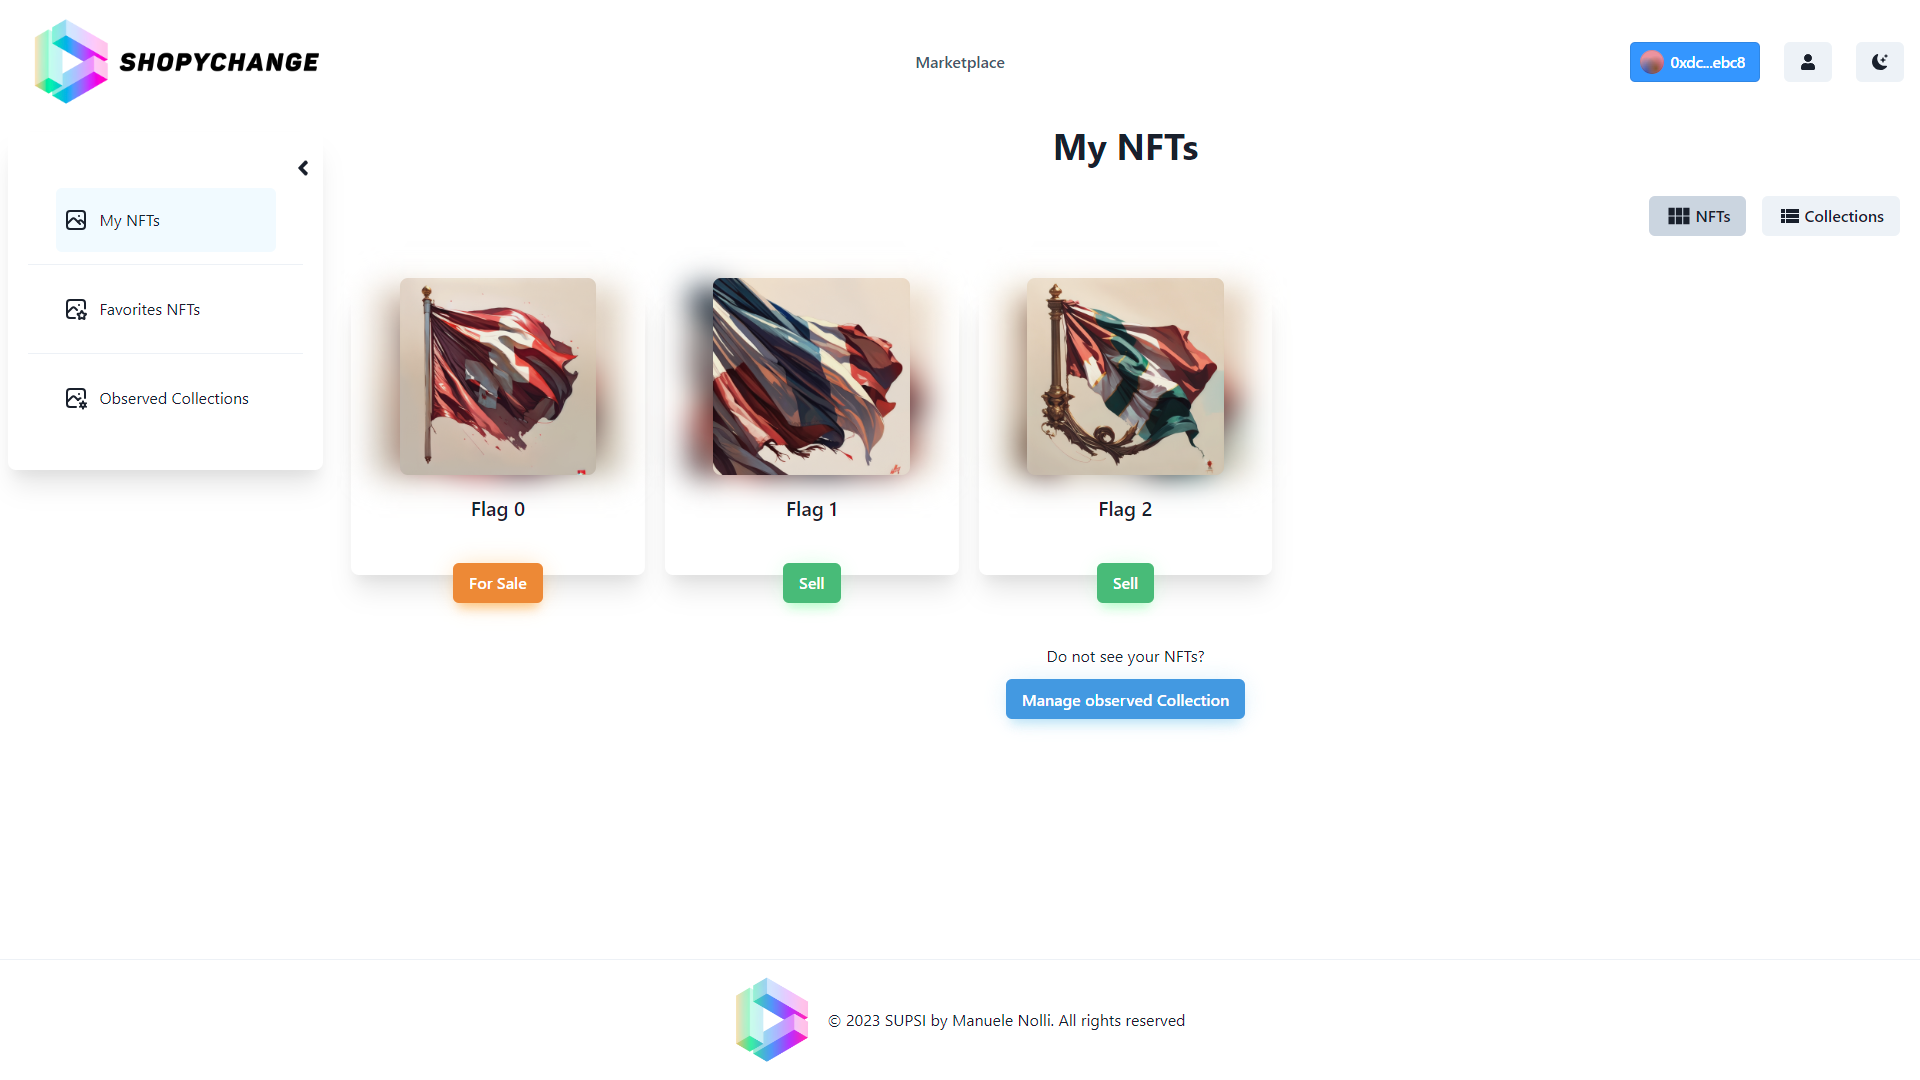
\includegraphics[width=\textwidth]{images/pages/myNFT.png}}
    \end{minipage}
    \hfill
    \begin{minipage}{0.26\textwidth }
      \centering
      \fcolorbox{mint-cream}{white}{
\includegraphics[width=\textwidth]{images/pages/myNFT_mobile.png}}
      \end{minipage}
      \caption{Pagina Account}
      \label{fig:account}
  \end{figure}

\subsubsection{Creazione}
\label{sec:creazione}

La pagina \textit{Creazione} è raggiungibile tramite il pulsante Account nell'header, il suo scopo è tramite due grandi pulsanti di direzionare l'utente alla pagina di creazione di un NFT o di una collezione. Le due pagine sono visibili nelle figure \ref{fig:create-nft} e \ref{fig:create-collection}. Entrambe contengono un form per l'inserimento dei dati e la possibilità di caricare una o più immagini. Il form è completamente validato e non permette l'invio di dati errati. 

\begin{figure}[H]
    \begin{minipage}{0.7\textwidth}
      \centering
      \fcolorbox{mint-cream}{white}{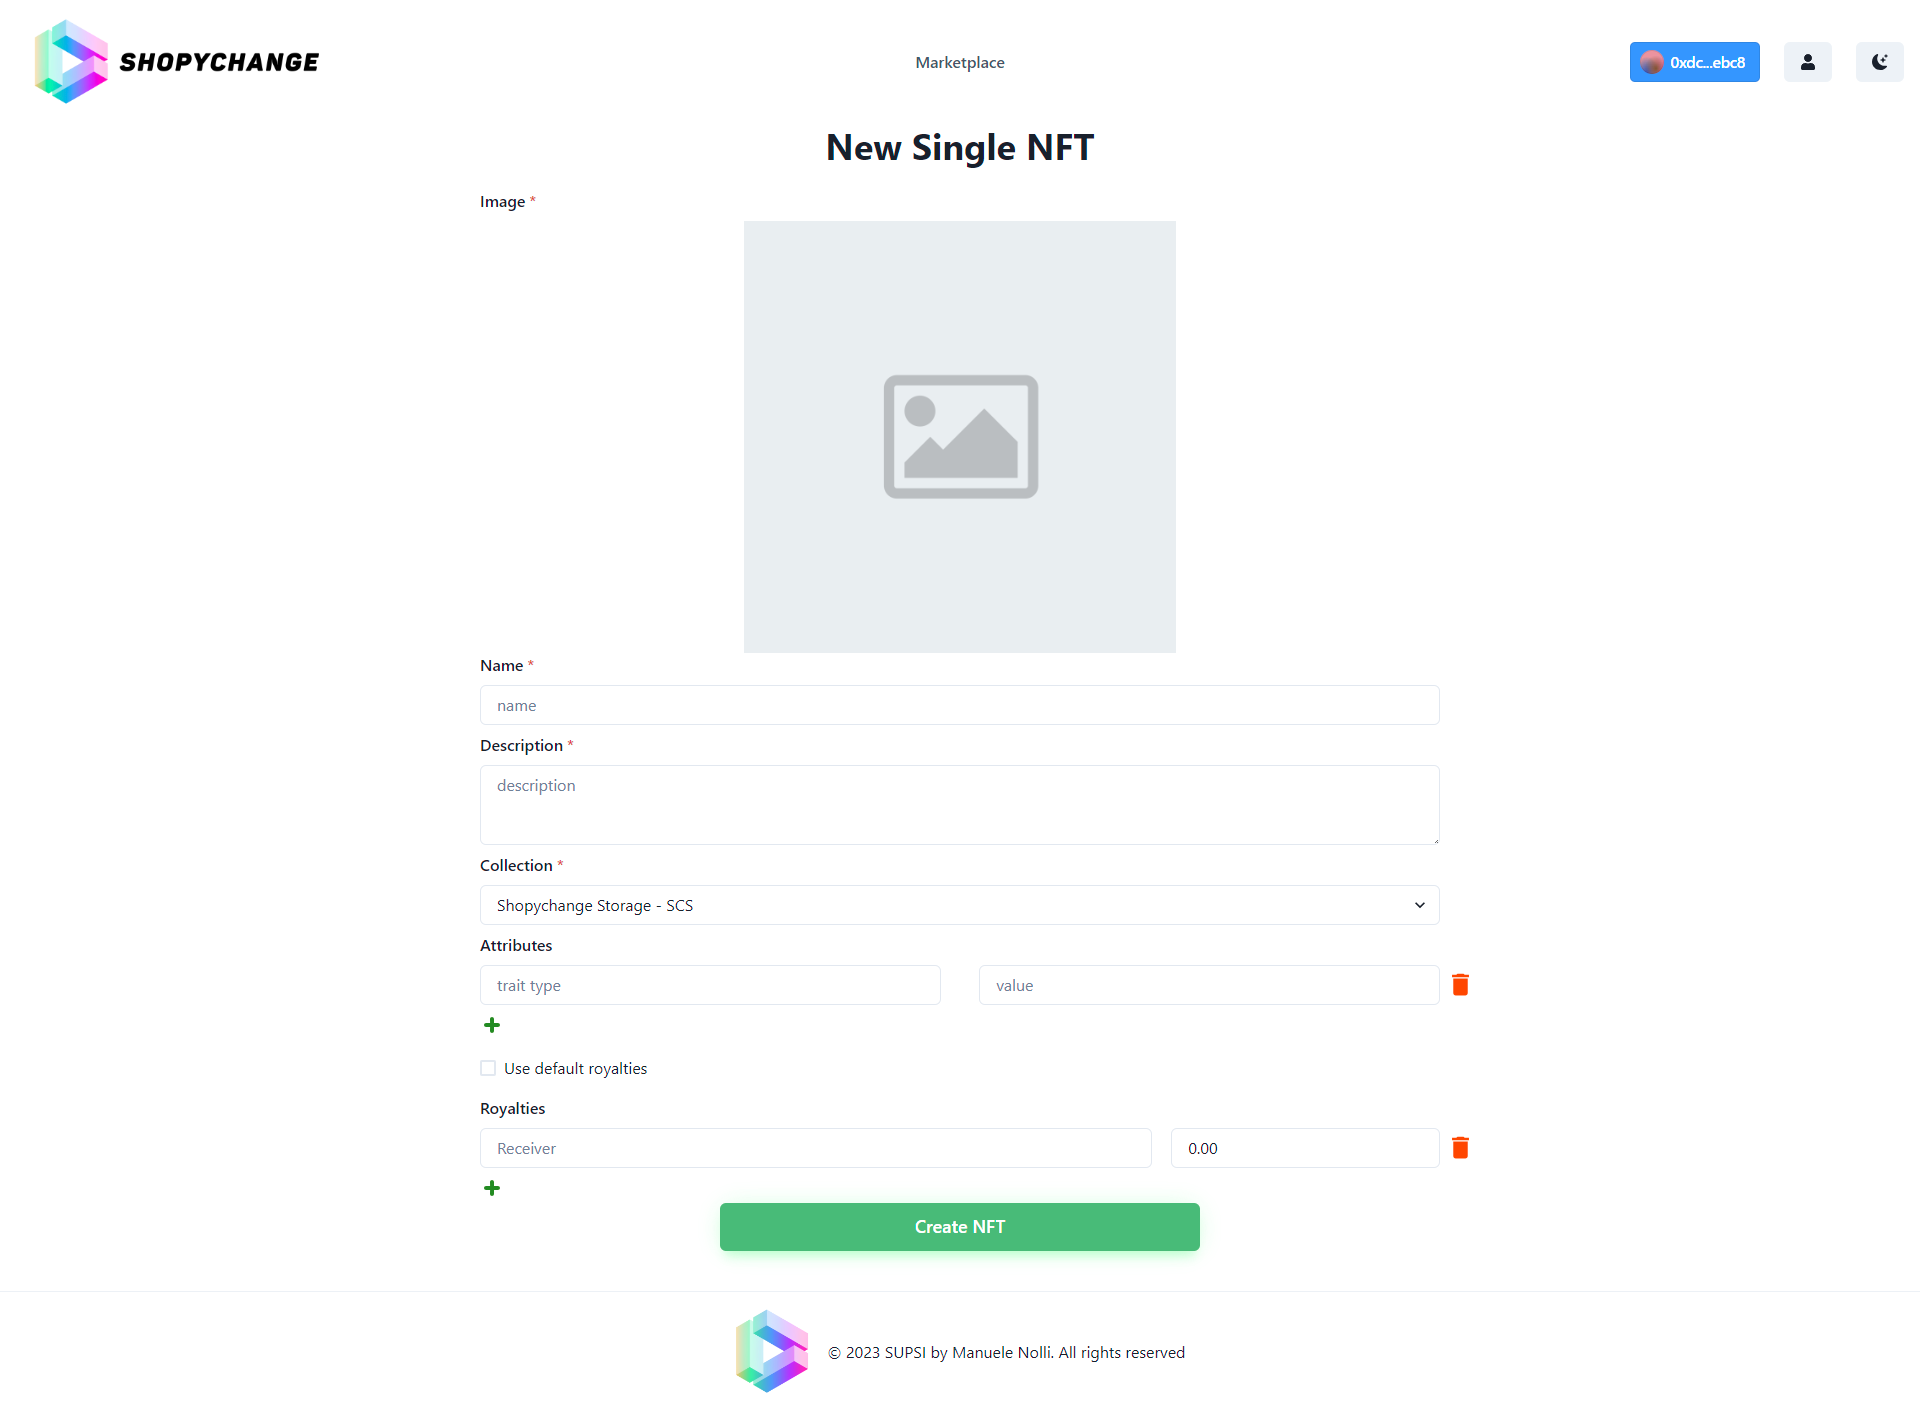
\includegraphics[width=\textwidth]{images/pages/createNFT.png}}
    \end{minipage}
    \hfill
    \begin{minipage}{0.26\textwidth }
      \centering
      \fcolorbox{mint-cream}{white}{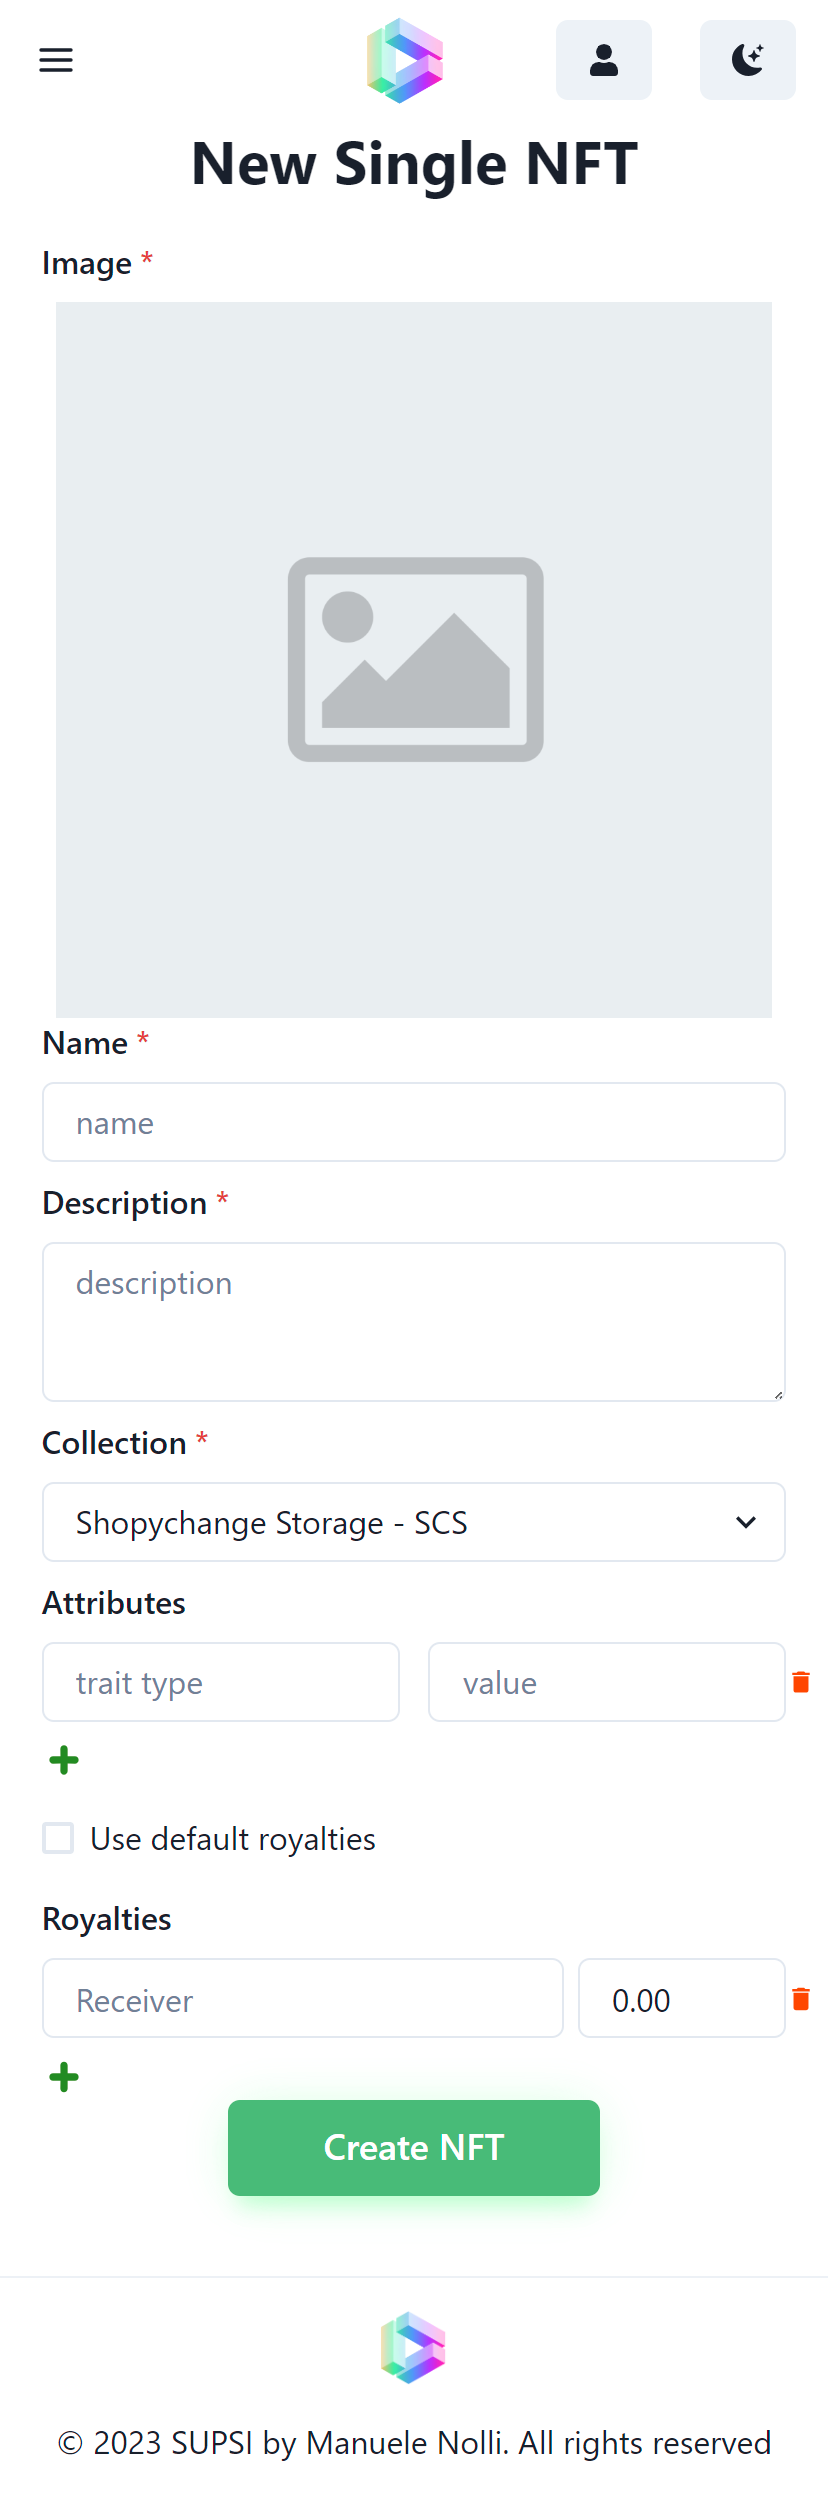
\includegraphics[width=\textwidth]{images/pages/createNFT_mobile.png}}
      \end{minipage}
      \caption{Pagina Creazione NFT}
      \label{fig:create-nft}
  \end{figure}

\begin{figure}[H]
    \begin{minipage}{0.7\textwidth}
      \centering
      \fcolorbox{mint-cream}{white}{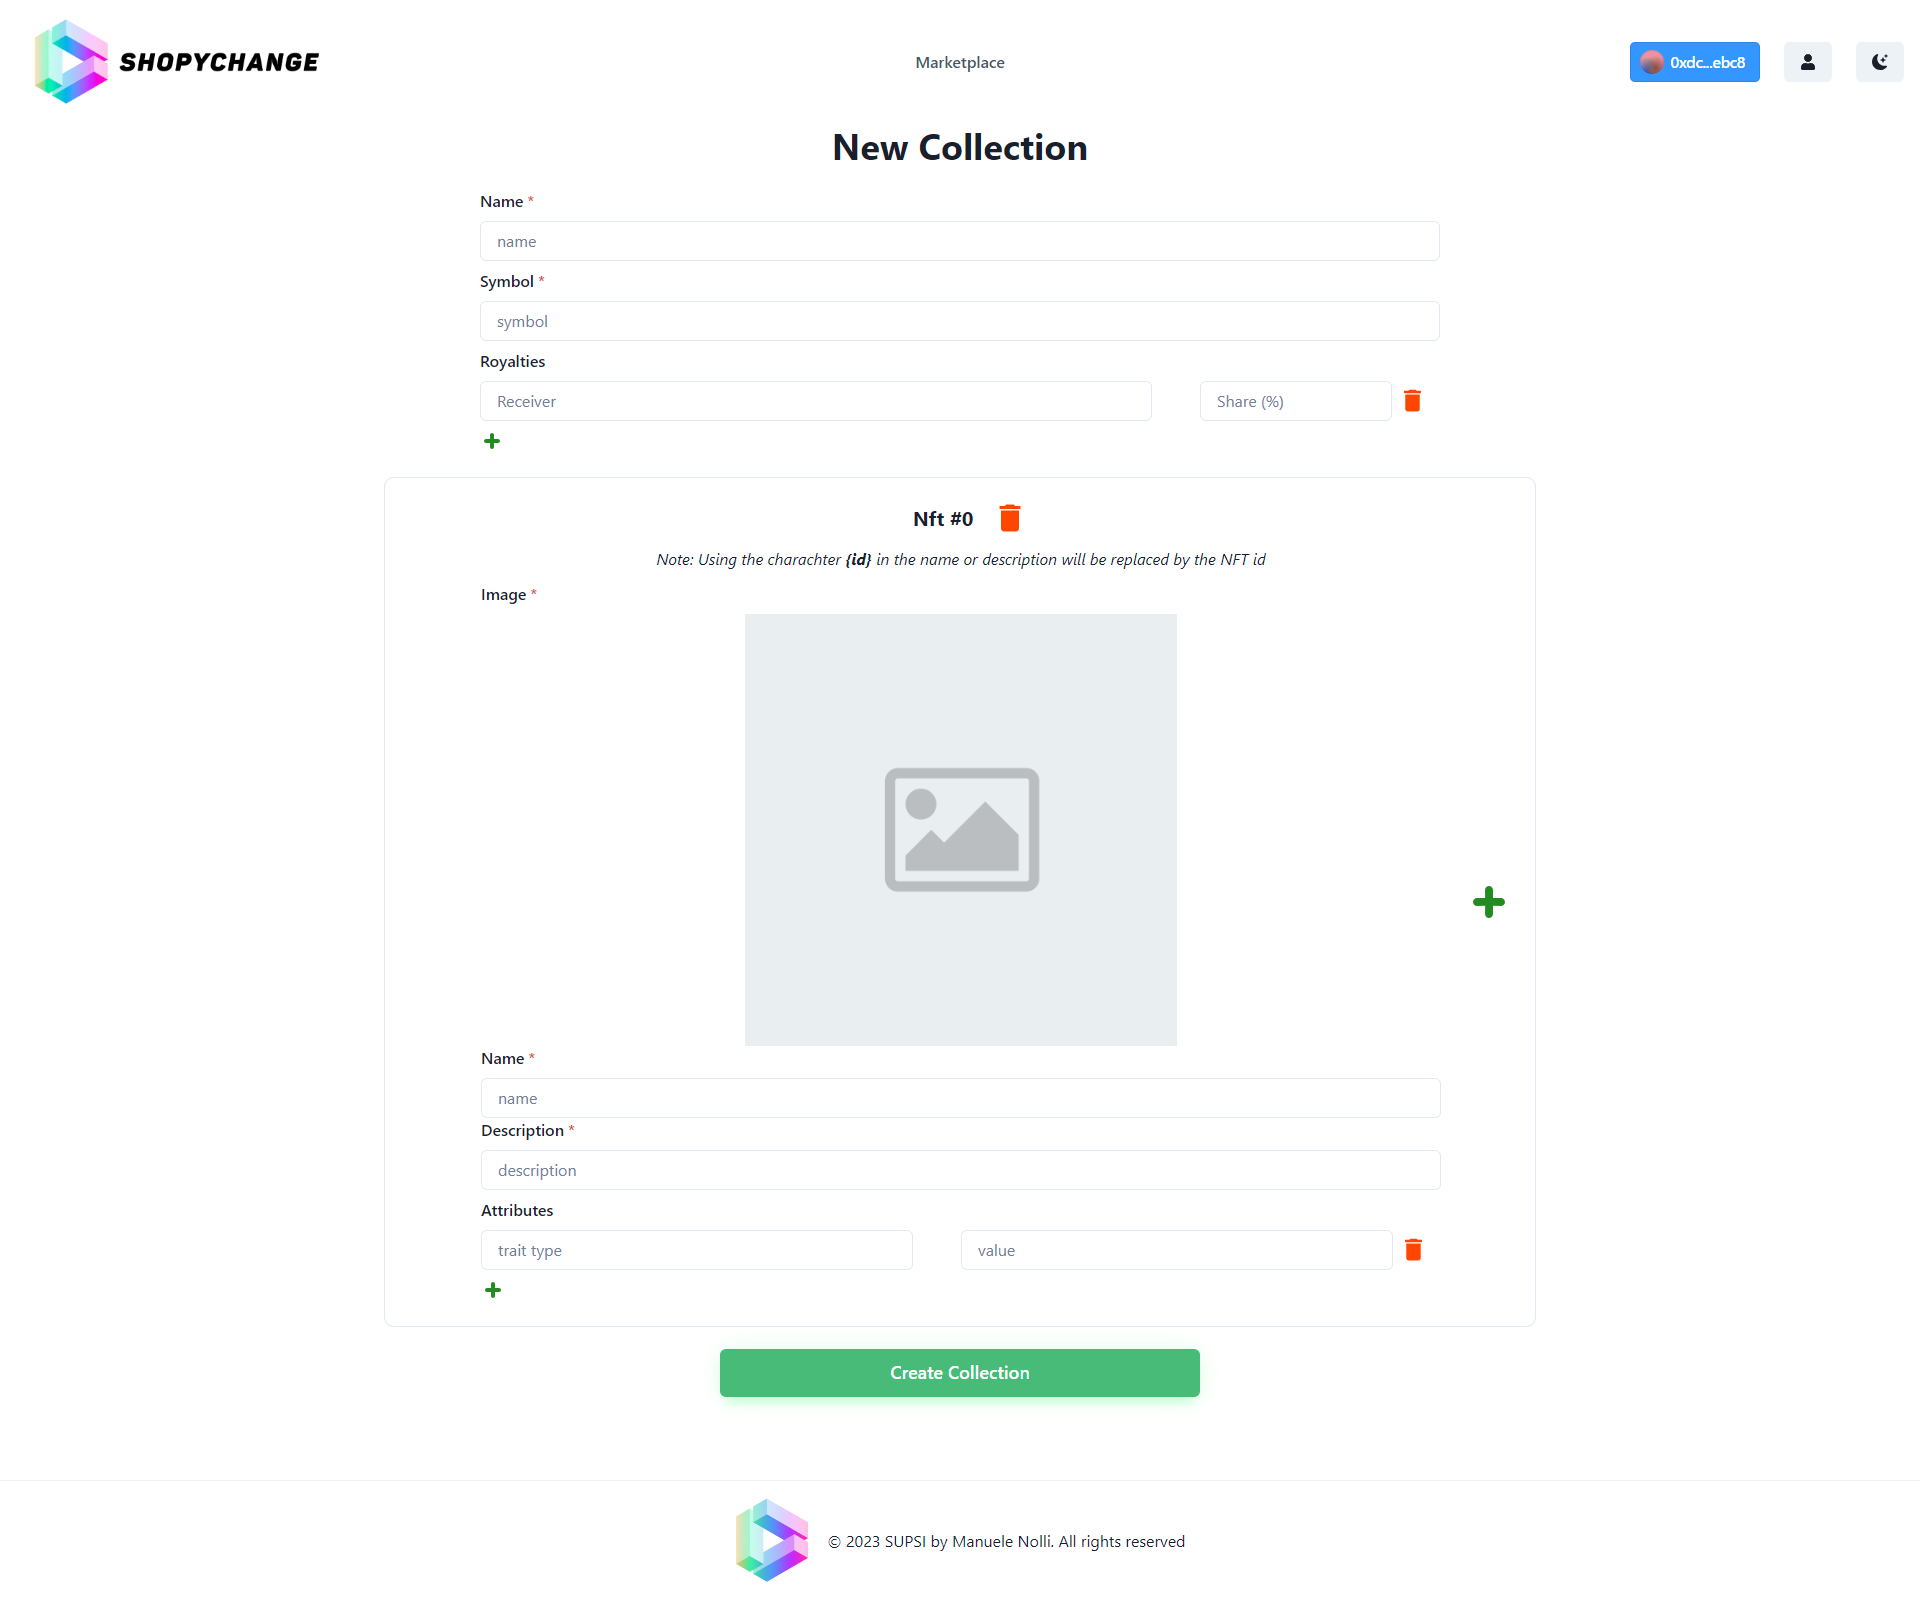
\includegraphics[width=\textwidth]{images/pages/createCollection.png}}
    \end{minipage}
    \hfill
    \begin{minipage}{0.26\textwidth }
      \centering
      \fcolorbox{mint-cream}{white}{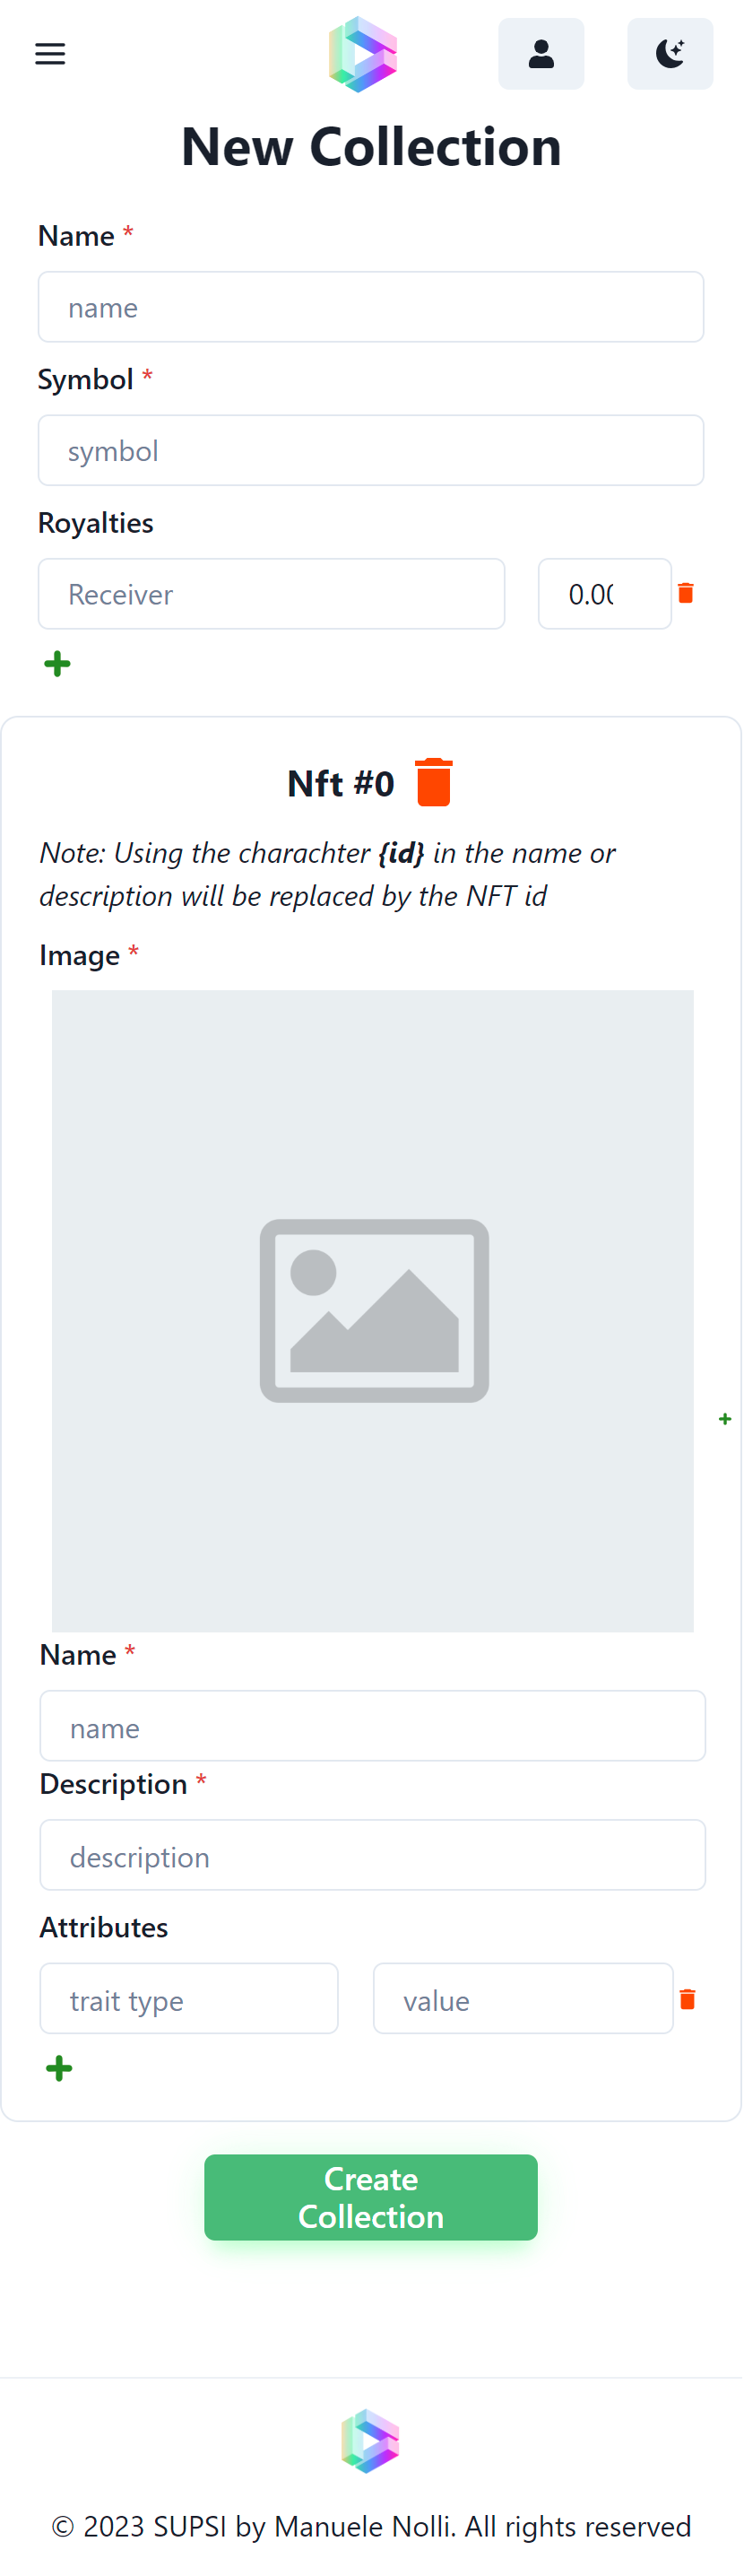
\includegraphics[width=\textwidth]{images/pages/createCollection_mobile.png}}
      \end{minipage}
      \caption{Pagina Creazione collezione}
      \label{fig:create-collection}
  \end{figure}

\subsubsection{Visualizzazione NFT} 

La seguente pagina permette di visualizzare tutte le informazioni riguardo ad un NFT. Ovvero, i dati del contratto, l'attuale possessore, i metadati dell'NFT e la cronologia di spostamento. Inoltre, la pagina cambia aspetto in base all'utente connesso e allo stato dell'NFT. La pagina è visibile con tema scuro in figura \ref{fig:visualizzazione-nft}.

\begin{figure}[H]
    \begin{minipage}{0.7\textwidth}
      \centering
      \fcolorbox{mint-cream}{white}{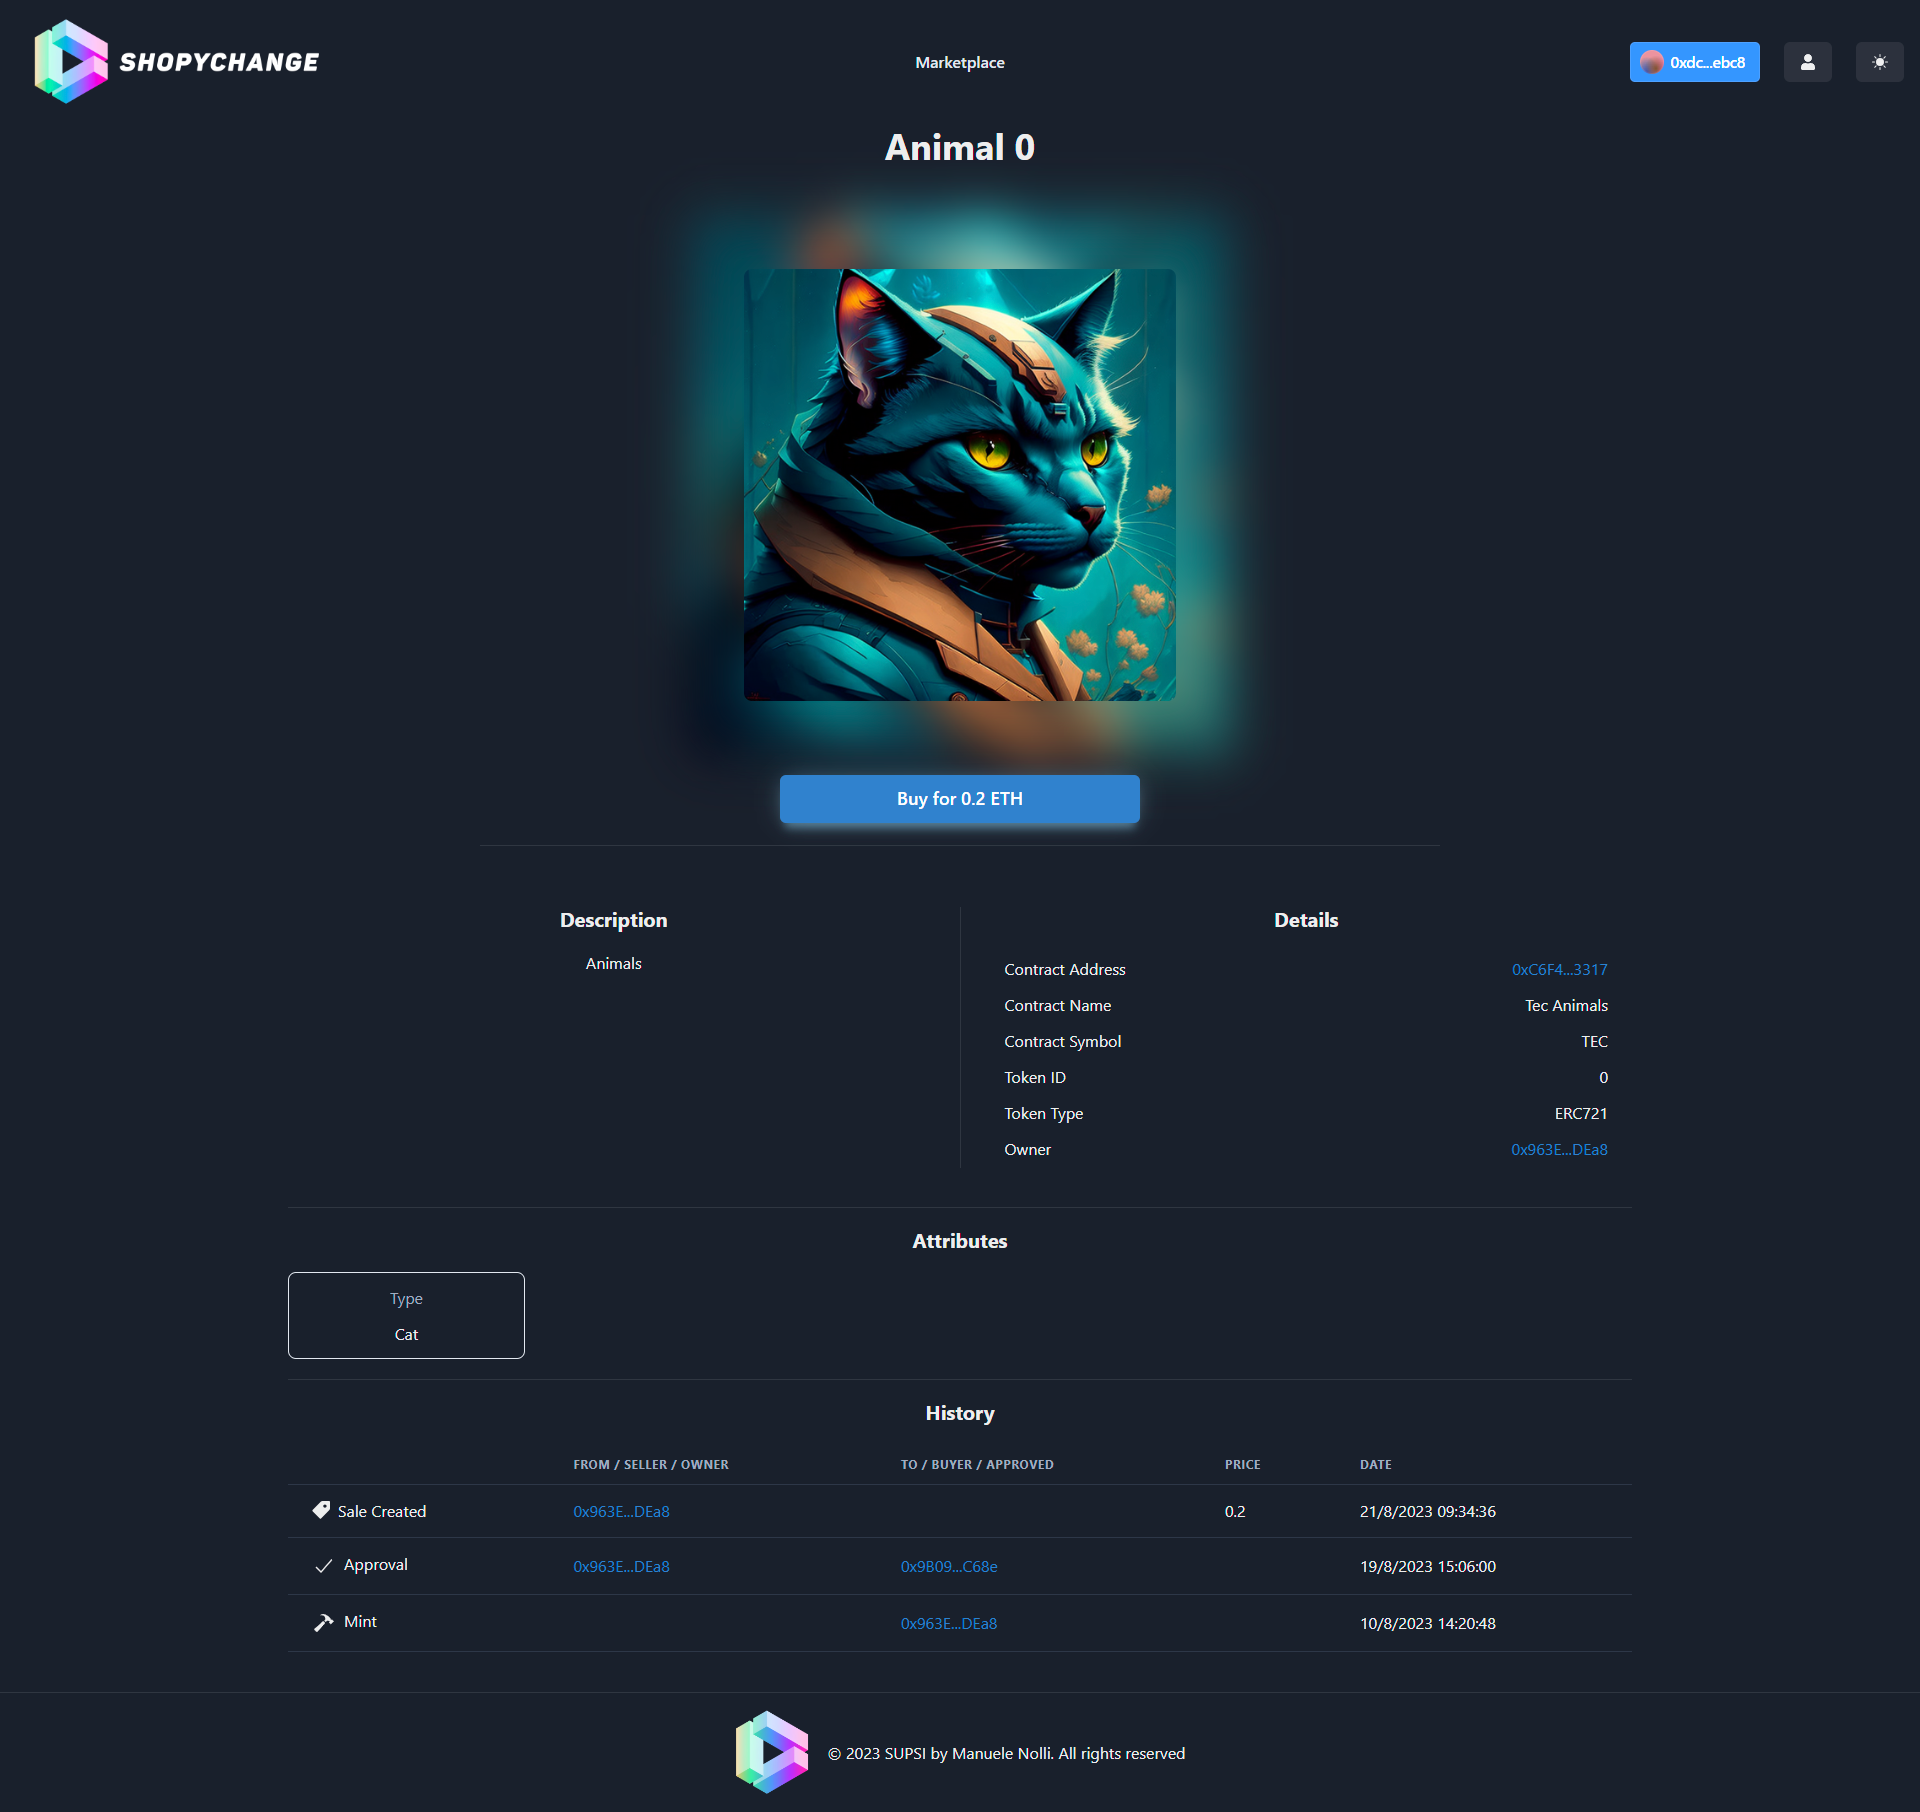
\includegraphics[width=\textwidth]{images/pages/nftPage.png}}
    \end{minipage}
    \hfill
    \begin{minipage}{0.26\textwidth }
      \centering
      \fcolorbox{mint-cream}{white}{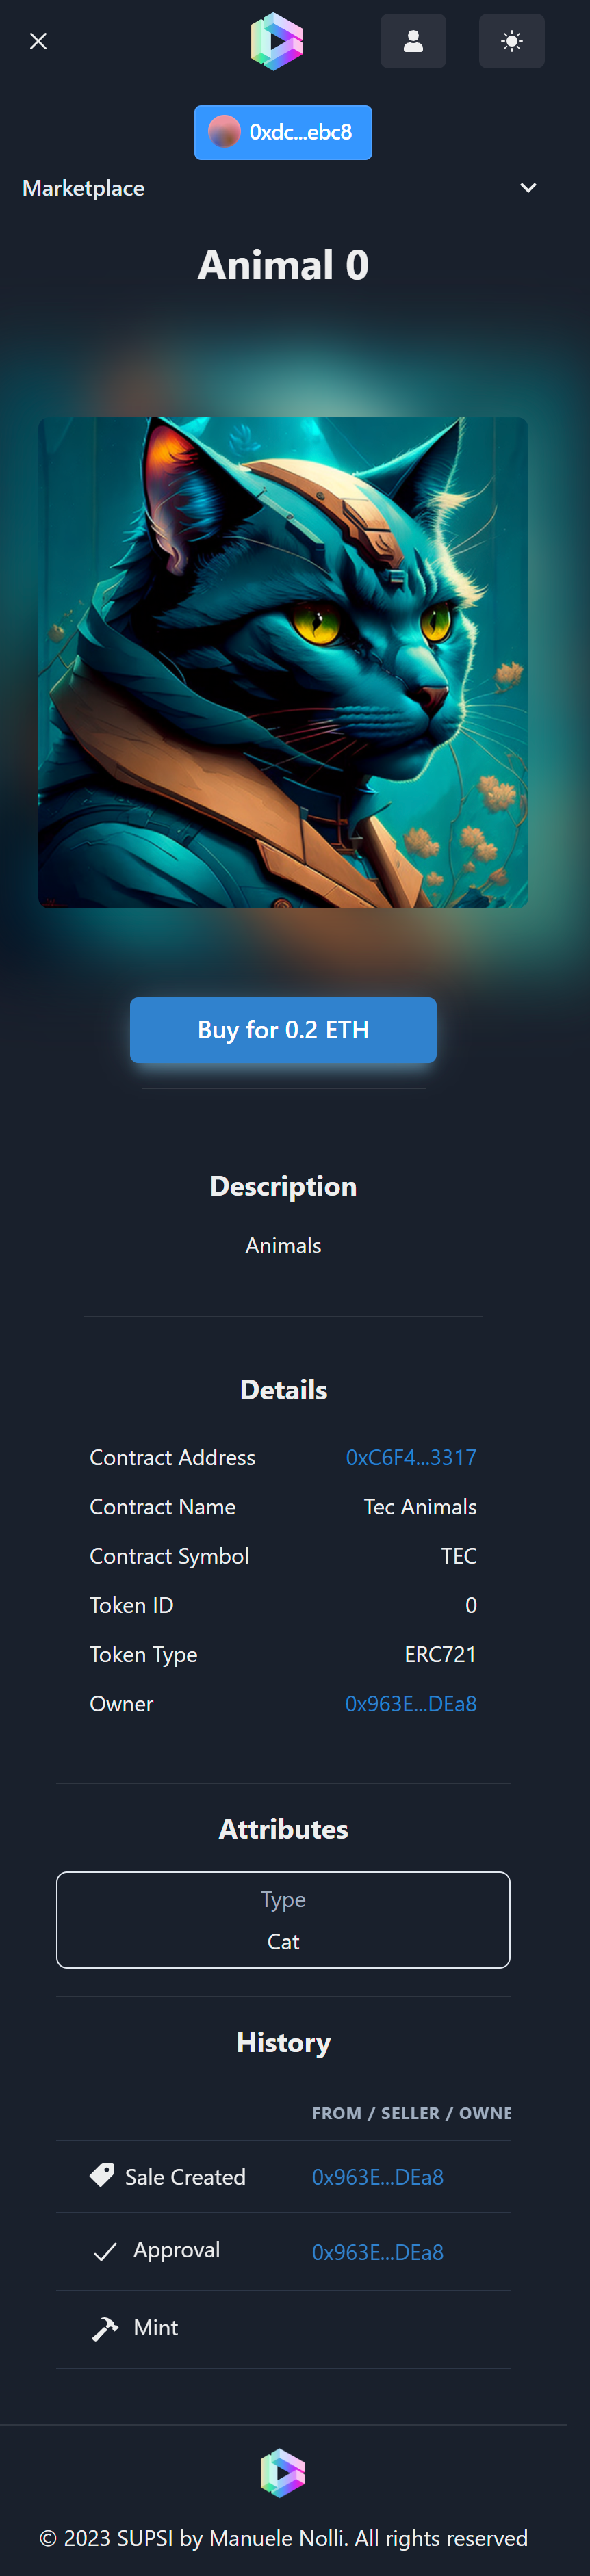
\includegraphics[width=\textwidth]{images/pages/nftPage_mobile.png}}
      \end{minipage}
      \caption{Pagina Visualizzazione NFT}
      \label{fig:visualizzazione-nft}
  \end{figure}

\subsubsection{Vendita, Acquisto, Modifica e Cancellazione}

Le operazione di messa vendita, acquisto, modifica e cancellazione di una vendita sono gestite tramite modali. Perciò, non è presente una pagina dedicata a queste operazioni ma sono presenti in diverse pagine. La figura \ref{fig:modal} mostra un esempio di messa in vendita di un NFT. Come è possibile notare, il modale presenta una tabella con le informazioni riguardanti alla divisione del prezzo di vendita. 

\begin{figure}[H]
    \begin{minipage}{0.7\textwidth}
      \centering
      \fcolorbox{mint-cream}{white}{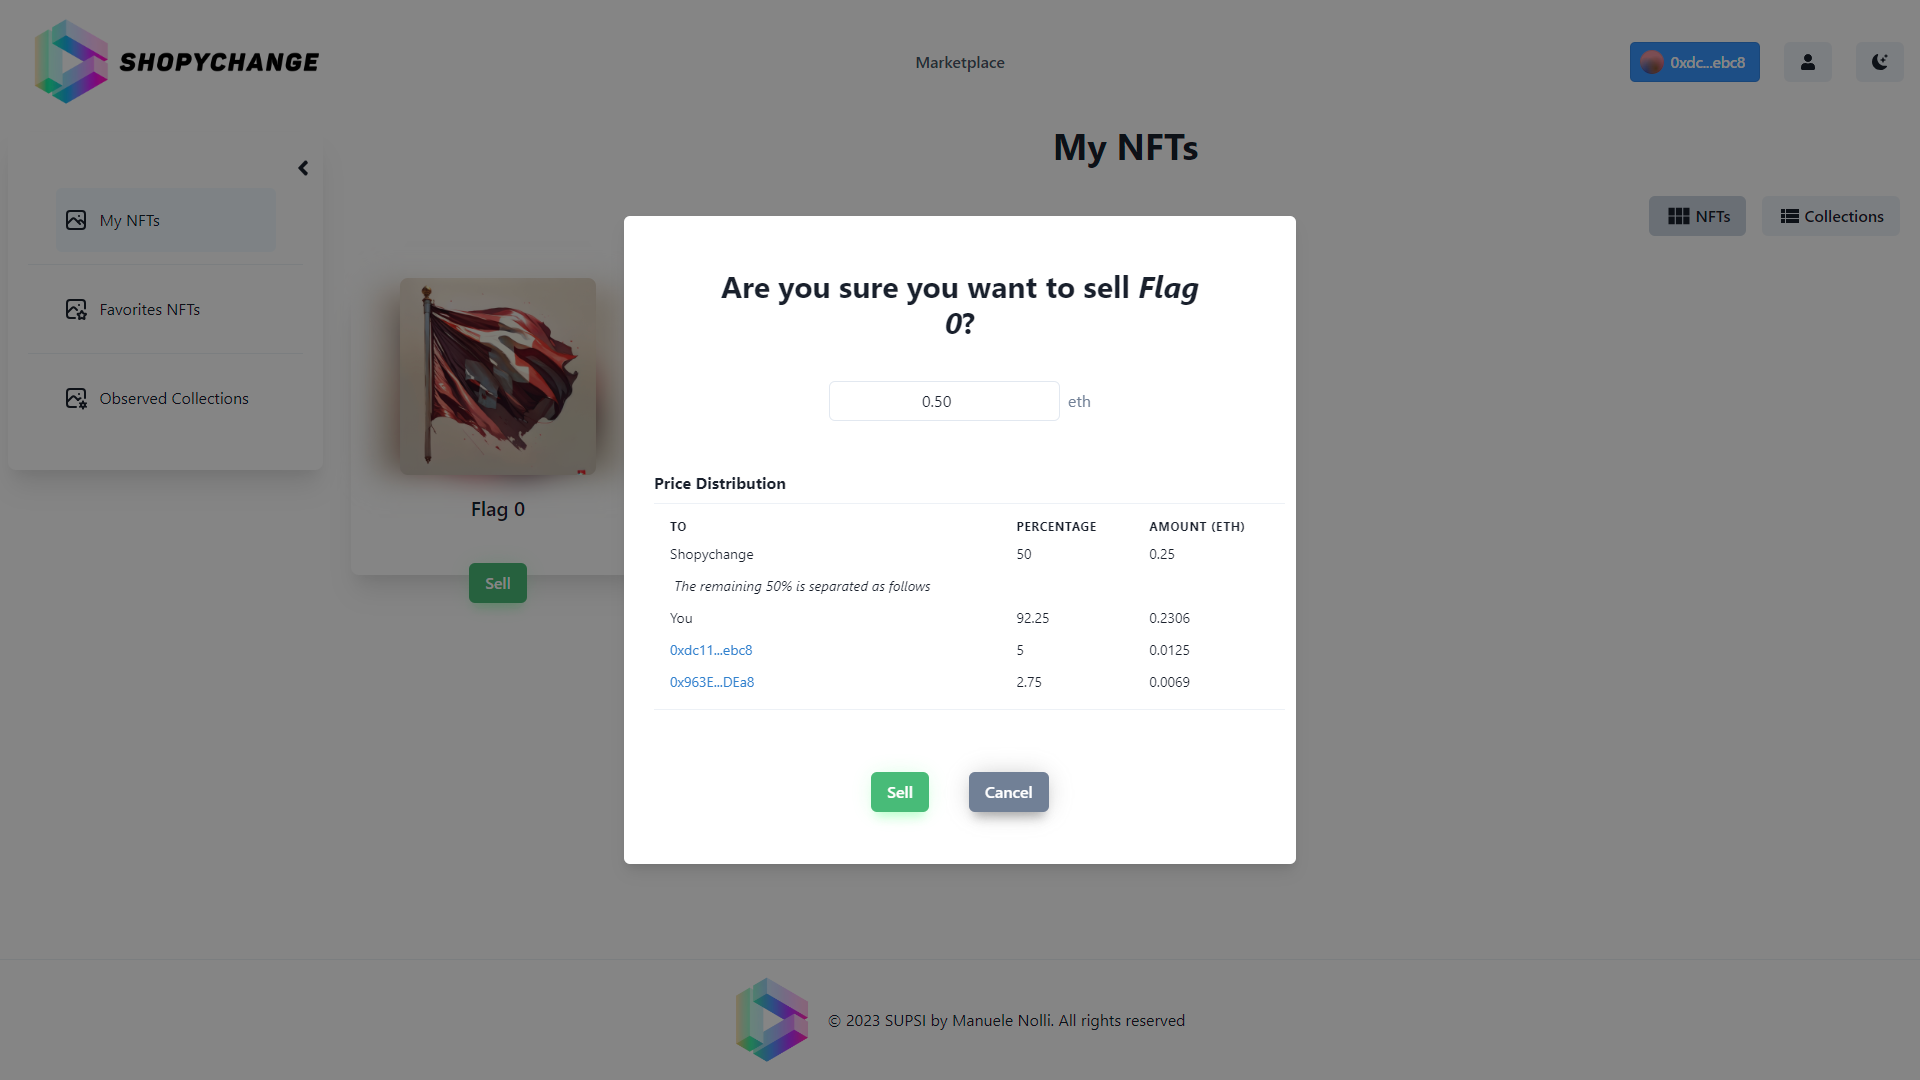
\includegraphics[width=\textwidth]{images/pages/sell.png}}
    \end{minipage}
    \hfill
    \begin{minipage}{0.26\textwidth }
      \centering
      \fcolorbox{mint-cream}{white}{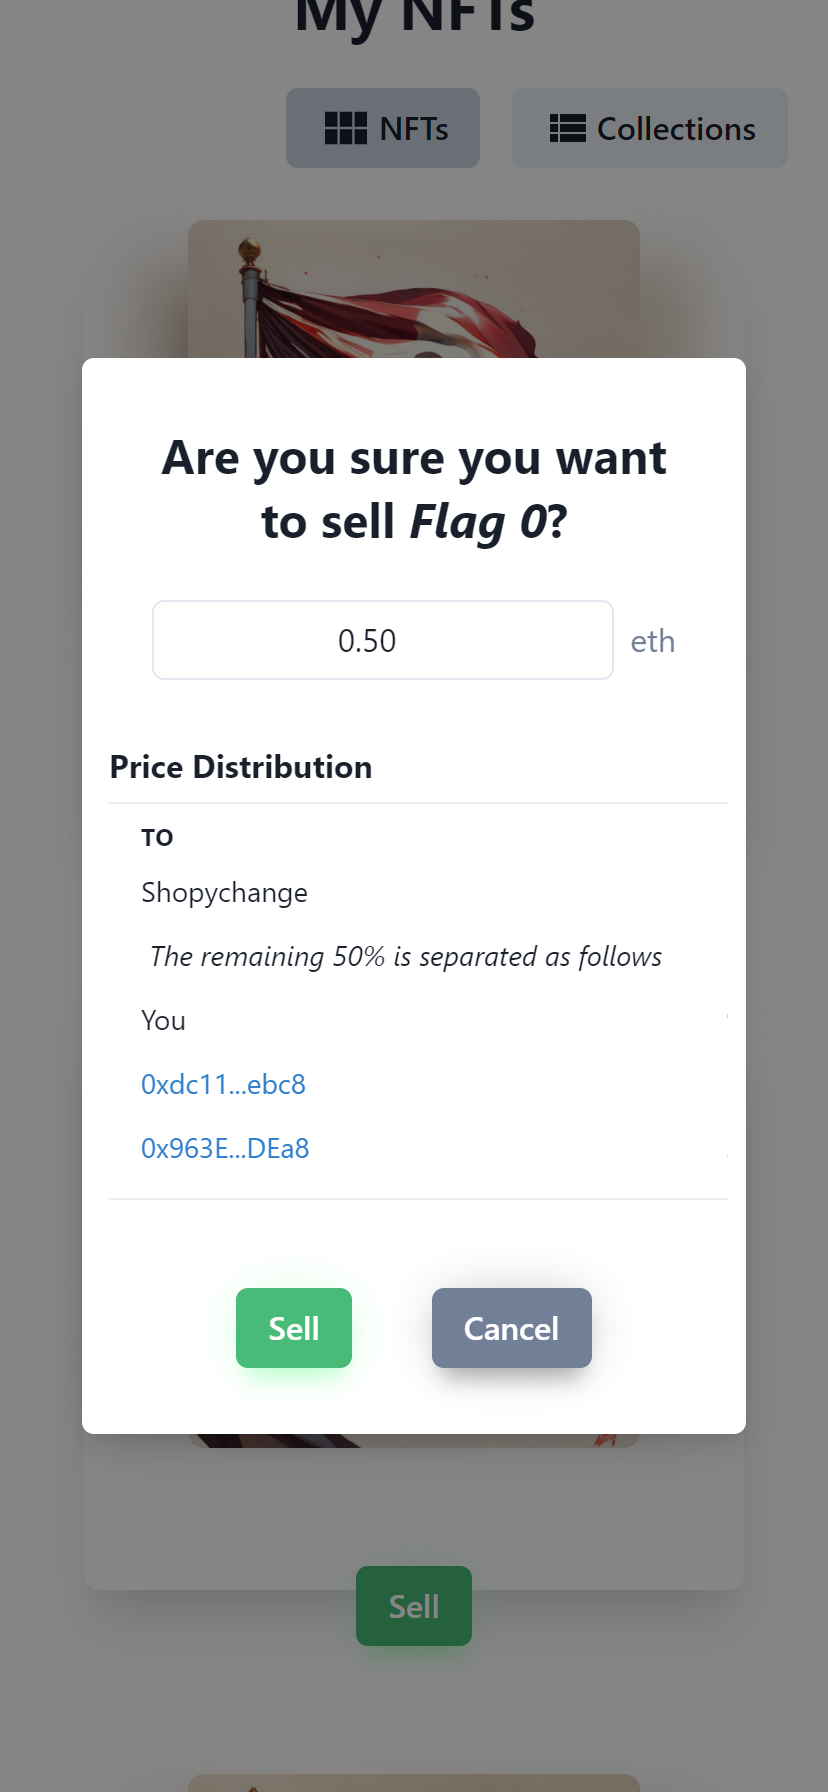
\includegraphics[width=\textwidth]{images/pages/sell_mobile.png}}
      \end{minipage}
      \caption{Modale Acquisto NFT}
      \label{fig:modal}
  \end{figure}

\subsubsection{Modifica Royalty}

  L'applicativo presenta due pagine per la modifica delle royalty. La prima rappresenta la modifica delle royalty di default per la collezione intera. La seconda pagina, visibile in figura \ref{fig:modifica-royalty}, permette di modificare le royalty di un singolo NFT, sganciandosi dalla royalty di default.

  \begin{figure}[H]
    \begin{minipage}{0.7\textwidth}
      \centering
      \fcolorbox{mint-cream}{white}{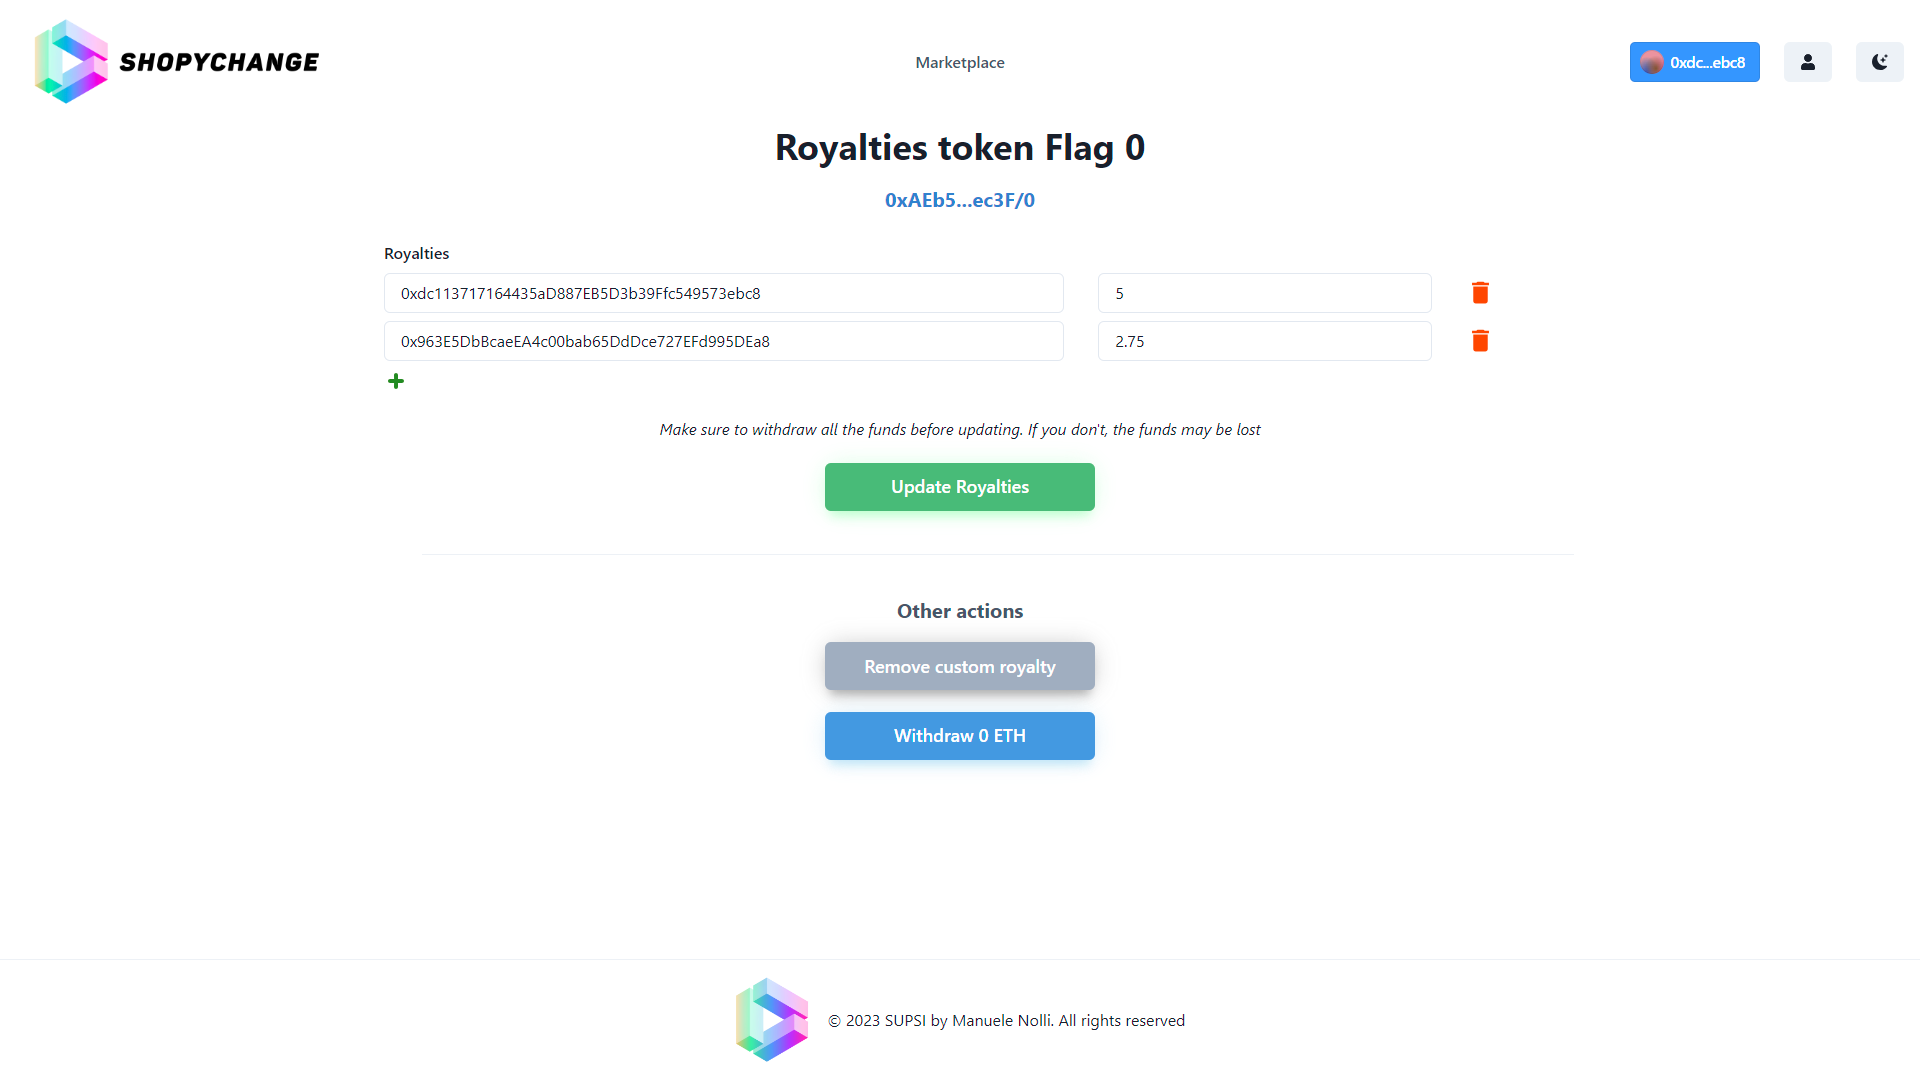
\includegraphics[width=\textwidth]{images/pages/tokenRoyalty.png}}
    \end{minipage}
    \hfill
    \begin{minipage}{0.26\textwidth }
      \centering
      \fcolorbox{mint-cream}{white}{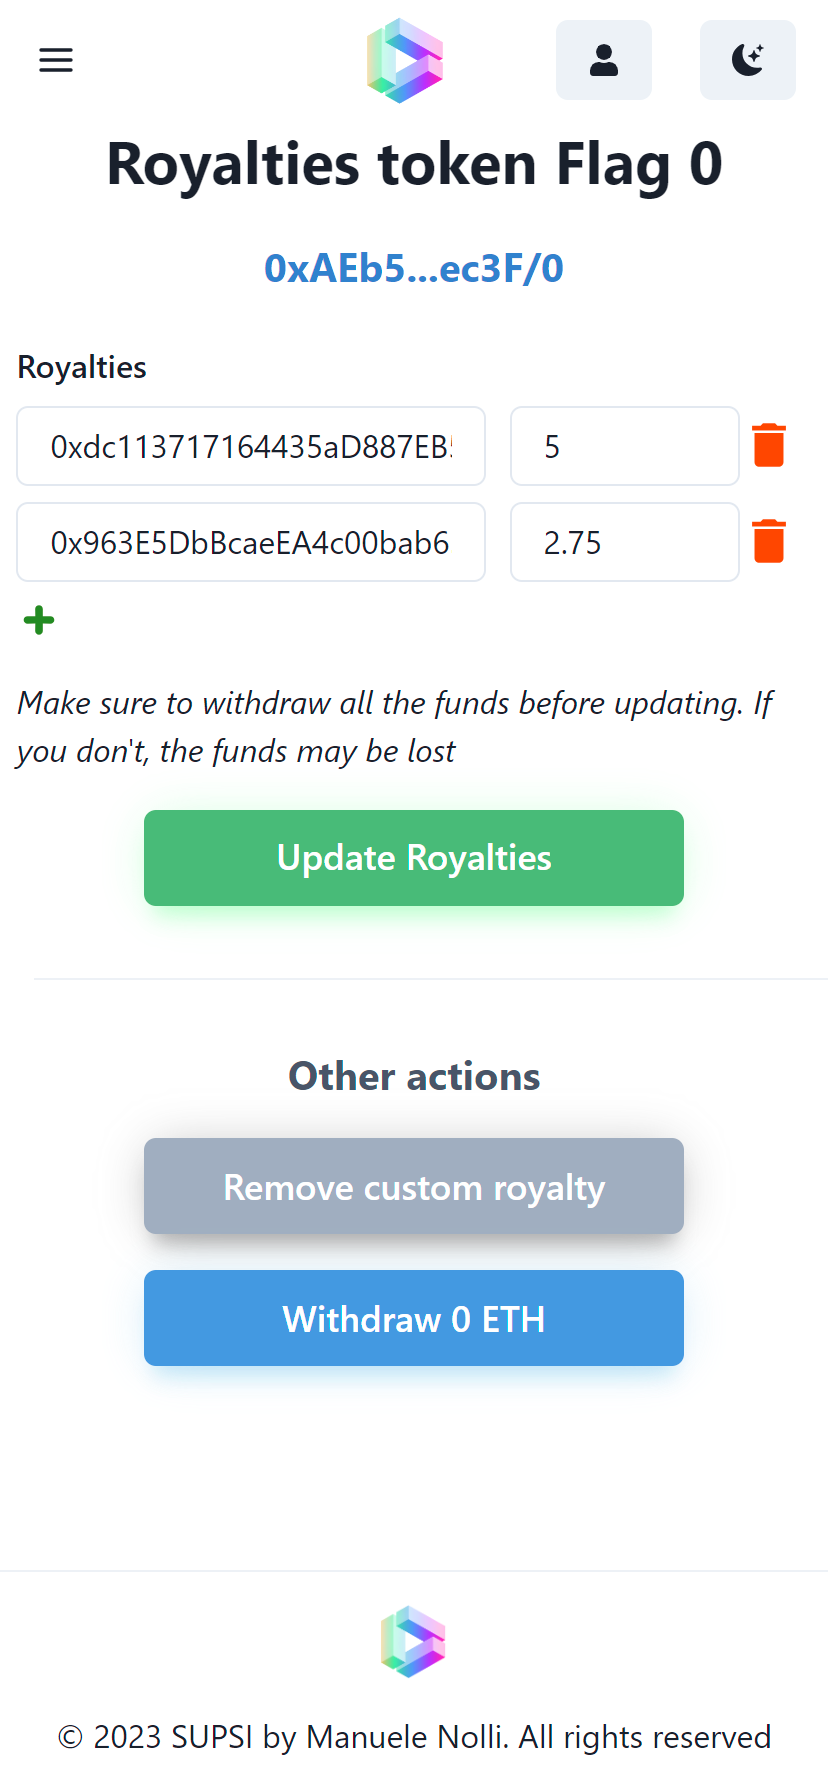
\includegraphics[width=\textwidth]{images/pages/tokenRoyalty_mobile.png}}
      \end{minipage}
      \caption{Pagina Modifica Royalty NFT}
      \label{fig:modifica-royalty}
  \end{figure}

\subsubsection{Admin dashboard}
\label{sec:admin-dashboard}

La pagina \textit{Admin} è raggiungibile unicamente dall'amministratore del marketplace. Al suo interno sono presenti le operazioni per il ritiro e modifica delle royalty a favore del marketplace, oltre a svariate funzionalità di gestione. La pagina è visibile in figura \ref{fig:admin}.

\begin{figure}[H]
    \centering
    \fcolorbox{mint-cream}{white}{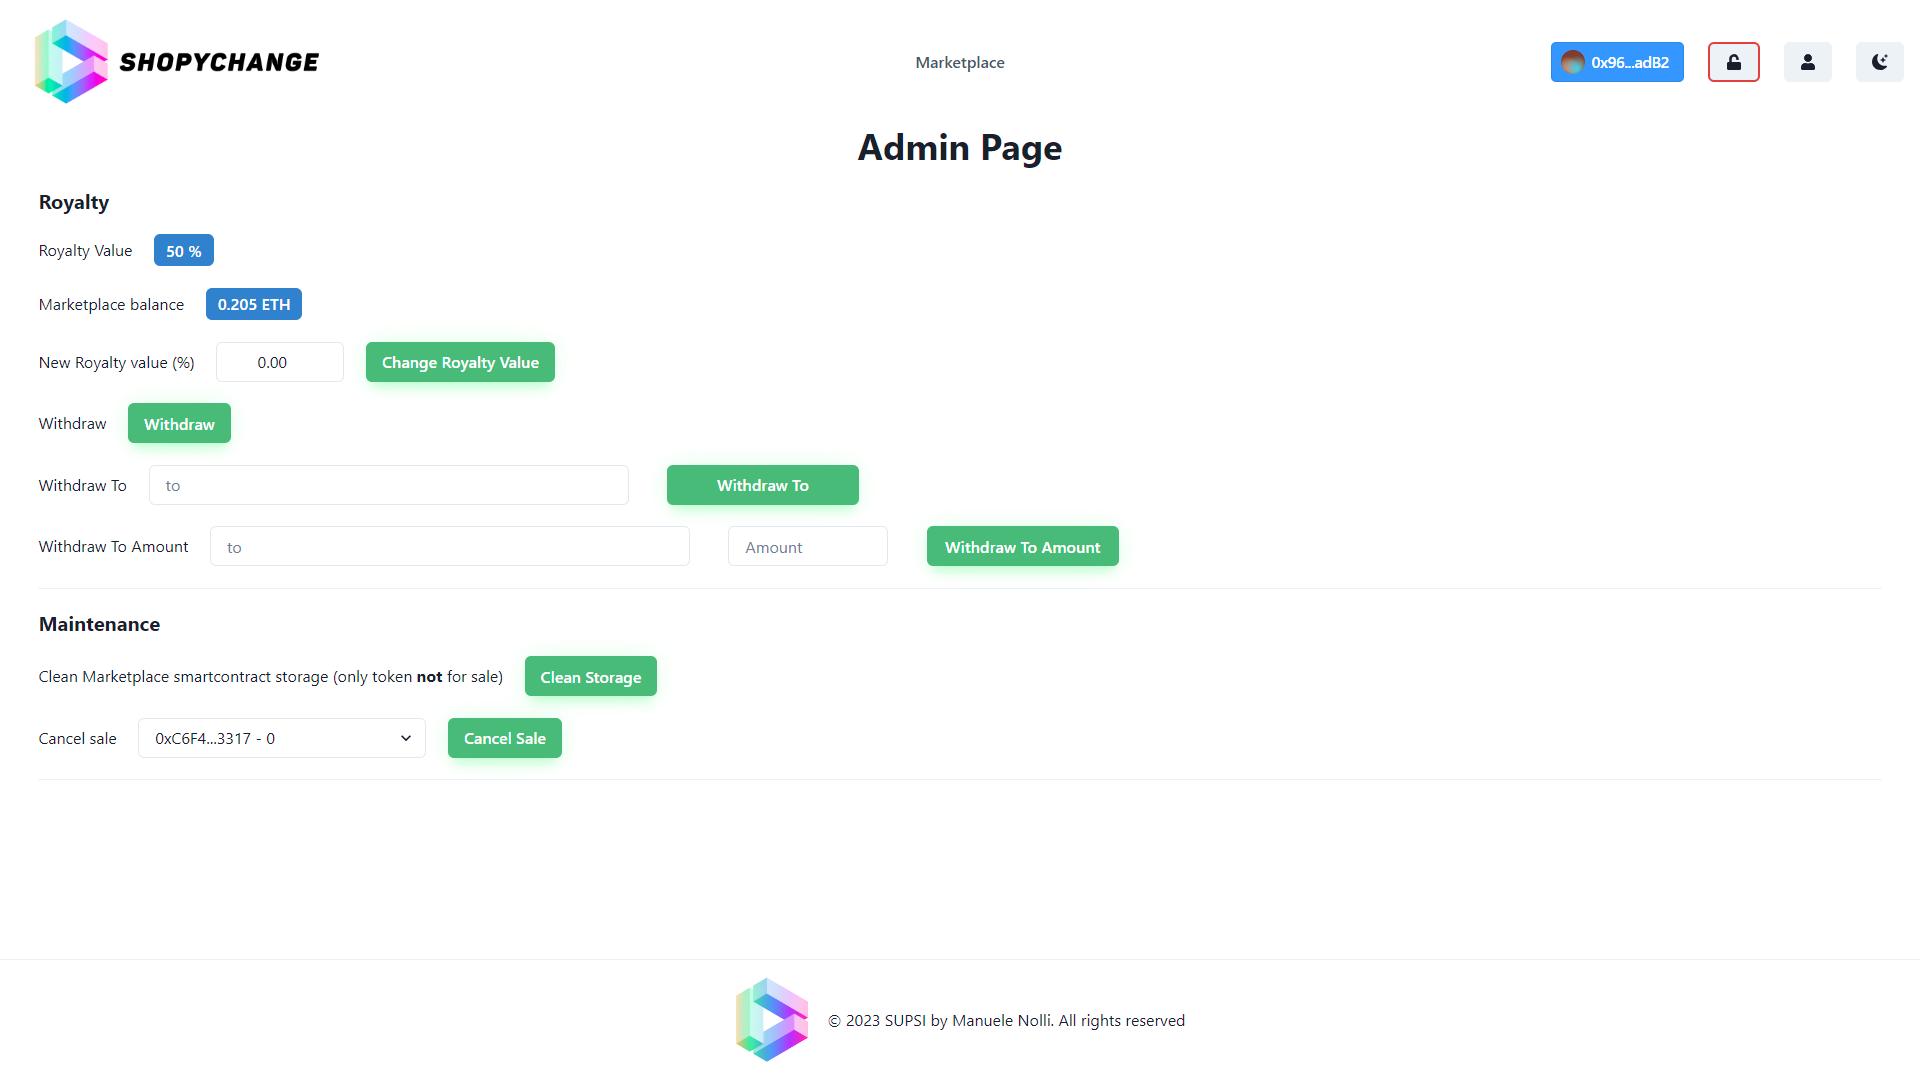
\includegraphics[width=0.8\textwidth]{images/pages/adminPage.png}}
    \caption{Pagina admin}
    \label{fig:admin}
\end{figure}

\subsection{Test}

Grazie all'organizzazione strutturale descritta nei precedenti capitoli ogni operazione è stata testata in modo efficace. I test sono stati scritti grazie all'aiuto della libreria \textit{jest}\footnote{https://jestjs.io/}, la quale permette di creare \textit{unit test}, \textit{snapshot test} e \textit{integration test}. Infatti, i test creati verificano la corretta visualizzazione grafica, il funzionamento in modo indipendente e l'integrazione con altri componenti.

In aggiunta, è stato utilizzato lo strumento \textit{Cypress}\footnote{https://www.cypress.io/} per la creazione di \textit{end-to-end test}. Questi test permettono di simulare l'interazione dell'utente con l'applicazione e di conseguenza di verificare il corretto funzionamento dell'applicativo. \textit{Cypress} è stato utilizzato in combinazione con \textit{Synpress}\footnote{https://github.com/Synthetixio/synpress}, ovvero uno strumento che permette la configurazione del wallet \textit{Metamask} all'interno del browser indipendente di \textit{Cypress}. In questo modo è stato possibile testare anche le funzionalità che richiedono l'interazione con la blockchain. Purtroppo però, a causa dell'impossibilità di verificare il funzionamento del pulstante di \textit{WalletConnect}, che permette la connessione del wallet, non è stato possibile testare le funzionalità che richiedono l'interazione con la blockchain. 

\subsection{Motivazioni e Alternative}

Il requisito per il modulo \textit{frontend} comprendeva l'utilizzo di \textit{Javascript}, ma essendo \textit{Typescript} un superset è stato deciso di utilizzare quest'ultimo in modo da ridurre gli errori di programmazione grazie ai tipi. La scelta del framework è stata fatta in base alla compatibilità delle librerie di comunicazione con la blockchain. Le alternative erano \textit{Angular}\footnote{https://angular.io/} e \textit{Vue}\footnote{https://vuejs.org/} ma la libreria \textit{WalletConnect} è maggiormente compatibile con \textit{React}.
 
La libreria \textit{WalletConnect} è stata scelta per la sua semplicità d'uso e la sua compatibilità con diversi wallet. Inoltre, risulta essere un protocollo più maturo rispetto alla sua alternativa principale, cioè \textit{RainbowKit}\footnote{https://www.rainbowkit.com/} che è attualmente alla versione 1.0.9.

In aggiunta, avendo scelto \textit{WalletConnect} è consigliato utilizzare \textit{Wagmi} invece di \textit{ethers.js} o \textit{web3.js}, in quanto l'integrazione tra \textit{WalletConnect} e \textit{ethers.js} risulta essere più complessa.

Per quanto riguarda la libreria grafica, la scelta è stata personale in quanto esistono diverse alternative valide come \textit{Material UI}\footnote{https://material-ui.com/} e \textit{Ant Design}\footnote{https://ant.design/}. \textit{ChakraUI} è stata scelta per la completezza e grafica dei componenti.
\section{Ulteriori strumenti}

Durante lo sviluppo del progetto è stato necessario sviluppare degli strumenti aggiuntivi che facilitassero il lavoro e completassero le funzionalità del marketplace. Nei prossimi paragrafi verranno analizzati questi strumenti.

\subsection{Creazione automatica NFTs}

Nella fase iniziale del progetto, prima dell'aggiunta della funzionalità di creazione di un NFT, è stato necessario creare manualmente gli NFTs per poterli visualizzare all'interno del marketplace. Essendo la creazione di un NFT completo di immagine e metadati un'operazione lunga e ripetitiva, è stato deciso di creare uno script che automatizzasse questo processo. Con lungimiranza nella possibile evoluzione del progetto, è stato deciso di creare uno script che permettesse di creare una collezione autogenerando le immagini e i metadati, nonché di pubblicarli su IPFS e blockchain.

Le immagini vengono generate utilizzando più \textit{layer} sovrapposti e personalizzabili. Più in dettaglio, per ogni \textit{layer} è possibile definire un insieme di immagini, da cui verrà scelta una in modo casuale in base alla rarità definita per ogni immagine. Un esempio di immagine generata è mostrato in figura \ref{fig:esempio-immagine-generata}.

\begin{figure}[H]
    \centering
    
\includegraphics[width=1\textwidth]{images/NFTAutogenerato.png}
    \caption{Esempio di immagine generata}
    \label{fig:esempio-immagine-generata}
\end{figure}


Per quanto riguarda i metadati, questi vengono generati in base alle immagini scelte per ogni \textit{layer}. In seguito alla configurazione del nome e della descrizione della collezione, il file json contenente i metadati relativo alla figura \ref{fig:esempio-immagine-generata} è il seguente:

\begin{lstlisting}[basicstyle=\small]
    {
        "name": "Planet #18",
        "description": "Would you like to live here?",
        "image": "18.png",
        "attributes": [
          {
            "trait_type": "background",
            "value": "lightBlue"
          },
          {
            "trait_type": "planet",
            "value": "blueDouble"
          },
          {
            "trait_type": "flyingObjects",
            "value": "ufo"
          }
        ]
      }
\end{lstlisting}

Nel seguito del progetto è stata riutilizzata la funzionalità di aggiunta automatica dei metadati a IPFS e blockchain. Quindi, l'autogenerazione di immagini non è stata inserita all'interno del marketplace in quanto è spesso compito del creatore fornire i metadati e l'immagine del NFT. Tuttavia, la funzionalità potrebbe essere facilmente aggiunta in futuro.

\subsection{Controllo integrità NFT in vendita}
\label{sec:controllo-integrita-nft-in-vendita}

Nel momento in cui un utente mette in vendita un NFT, il marketplace diventa semplicemente un gestore dell'asset e non il suo possessore. Questo significa che l'utente ha il pieno controllo dell'asset. Infatti, se l'utente decidesse di trasferirlo esternamente al marketplace ad un altro indirizzo, il marketplace non sarebbe in grado di rilevare questo cambiamento e di conseguenza si verificherebbe un errore, come schematizzato in figura \ref{fig:integrita-nft}.


\begin{figure}[H]
    \centering
    \includegraphics[width=1\textwidth]{images/IntegritàNFT.png}
    \caption{Esempio di mancanza di integrità di un vendita}
    \label{fig:integrita-nft}
\end{figure}

Per risolvere tale problema è stato deciso di implementare un controllo di integrità di tutti gli NFT attualmente in vendita. Il microservizio creato analizza tutti i nuovi blocchi generati dalla blockchain, filtrando il contenuto su eventi di tipo \textit{transfer} emessi dai token in vendita. Nel caso in cui esista un evento di questo genere e non sia stato emesso l'evento di vendita dal marketplace, il microservizio invierà una transazione per rimuovere l'asset dalla vendita. In questo modo, il marketplace è sempre in grado di rilevare eventuali cambiamenti di proprietà degli NFT in vendita.
\section{Metolodogia di sviluppo}
Il progetto è stato sviluppato utilizzando la metodologia \textit{Agile}, in particolare è stato utilizzato il framework \textit{Scrum}, in modo da poter avere un'idea chiara dei requisiti e delle funzionalità che il sistema deve avere, così da poterle implementare in modo incrementale e iterativo. 

Gli \textit{Sprint} sono stati di due settimane, così da avere un costante feedback da parte del relatore.

\subsection{Git}
Lo strumento di versionamento utilizzato è \textit{Git} o più precisamente \textit{GitLab}. Questo strumento offre anche diverse funzionalità di supporto all'utilizzo di metodologie Agile. Infatti, i \textit{milestone} sono stati utilizzati per identificare gli \textit{Sprint} e le \textit{issue} per identificare i singoli task da svolgere. Queste ultime sono state divise in \textit{User Story} con lo scopo di essere connesse ai requisiti funzionali e non.

\subsection{CI/CD}

Grazie a \textit{Gitlab} è stato possibile utilizzare il \textit{Continuous Integration} e il \textit{Continuous Delivery} per automatizzare il processo di testing. Attraverso un file di configurazione chiamato \textit{.gitlab-ci.yml} è stato possibile calcolare la \textit{coverage} del codice e verificare che tutti i test avessero esito positivo. 
\chapter{Risultati}
\label{sec:risultati}

Nel seguente capitolo verranno presentati i risultati ottenuti e le riflessioni maturate durante lo sviluppo del progetto. Le tematiche trattate durante l'analisi e la progettazione del marketplace sono state molteplici, tra queste la gestione delle \textit{Artist's Resale Right} \cite{resale-right}, equivalente del \textit{revenue share} è stata la più complessa. 

La gestione delle \textit{royalties} è un tema attualmente molto discusso. Non essendoci uno standard completo i principali marketplace decentralizzati hanno adottato delle soluzioni personali per la loro implementazione. Le problematiche che affliggono questo argomento sono principalmente due: l'interoperabilità tra più marketplace e il rafforzamento della distribuzione delle \textit{royalty}. Lo standard \textit{ERC2981} risolve unicamente la prima problematica rendendolo non attrattivo, dato che per un marketplace risulta essere più importante l'\textit{enforcement} del \textit{revenue share}. Nel caso in cui un marketplace non riuscisse a garantire il pagamento delle \textit{royalties} al creatore dell'asset, quest'ultimo non sarà incentivato ad utilizzare la piattaforma. Proprio per questo motivo, i marketplace decentralizzati hanno adottato soluzioni proprietarie per garantire l'\textit{enforcement} del \textit{revenue share}, ma non essendo interoperabili tra loro l'ecosistema decentralizzato risulta essere frammentato. In aggiunta, ottenere informazioni tecniche sulle soluzioni adottate è un processo arduo, il che può generare dei dubbi sulla loro effettiva affidabilità. Di seguito è presente la tabella \ref{table:implementazioni-royalty} che riassume le differenze sovracitate.


\begin{table}[H]
    \centering
    \renewcommand{\arraystretch}{1.5}
    \begin{adjustbox}{max width=1\textwidth}
        \begin{tabular}{| p{0.33\linewidth} | p{0.33\linewidth} | p{0.33\linewidth} |}
            \hline
            \rowcolor{mint-cream}
                                             & Interoperabilità                                                       & Enforcement                                      \\
            \hline
            Utilizzo di ERC2981             & Presente ma lo standard ERC2981 non è largamente utilizzato            & Se presente, unicamente sul marketplace in cui è stato creato l'asset \\
            \hline
            Soluzioni dei principali marketplace decentralizzati  & Spesso nessuna interoperabilità tra marketplace diversi & Asset scambiabile unicamente sul marketplace in cui è stato creato l'asset, quindi enforcement presente \\
            \hline
        \end{tabular}
    \end{adjustbox}
    \caption{Confronto implementazioni \textit{royalty}}
    \label{table:implementazioni-royalty}
\end{table}

Dal mio punto di vista, la soluzione migliore sarebbe avere uno standard completo che includa l'obbligo di pagamento e la distribuzione automatica delle \textit{royalties} non in maniera spontanea come avviene attualmente. Chiaramente la difficoltà tecnica risiede nell'impossibilità di modificare gli standard NFT già esistenti, ma essendo la tecnologia blockchain in uno stato di crescita e sviluppo, sarebbe riduttivo fermarsi e adattarsi per mantenere la compatibilità con gli attuali sistemi. Come descritto nel documento \textit{The Renaissance of Legacy Systems} \cite{warren2012renaissance} riguardante l'aggiornamento dei sistemi obsoleti, i tentativi di cambiamenti con le tecniche di manutenzione possono rivelarsi terribilmente costosi e non soddisfare i nuovi requisiti, poiché il sistema non è in grado di accogliere ulteriori funzionalità. In questo scenario, lo sforzo e i costi investiti nel sistema vanno sprecati. Sebbene le attuali soluzioni non siano perfette, sono comunque applicabili e adatte a dipendenza del contesto di utilizzo. Una tipologia di marketplace che potrebbe non necessitare di interoperabilità ma unicamente della certezza della suddivisione delle \textit{royalties} sono i marketplace proprietari, i quali vendono beni connessi ad un servizio da loro offerto. Questo genere di marketplace non è totalmente decentralizzato ma può beneficiare della sicurezza fornita dalla blockchain, nonché della garanzia di gestione delle \textit{royalties} concessa dagli smart contracts ma anche di ulteriori funzionalità personalizzate, come ad esempio il controllo sul prezzo di \textit{reselling}. Il mercato del gaming e dei ticket per eventi sono due esempi che potrebbero utilizzare un marketplace di questa tipologia. 


Analizzando più in dettaglio i marketplace di tipo decentralizzato, è possibile confermare che essi costituiscono enormi vantaggi in termine di sicurezza, privacy e trasparenza rispetto ai marketplace centralizzati. L'approccio verso la trasparenza è notabile all'interno della soluzione sviluppata, per esempio in figura \ref{fig:risultati_storico}, dove è visibile l'intero storico dell'asset, e in figura \ref{fig:risulati_royalty}, dove è possibile visualizzare la divisione delle \textit{royalties} all'acquisto di un asset.

\begin{figure}[H]
    \centering
    \fcolorbox{mint-cream}{white}{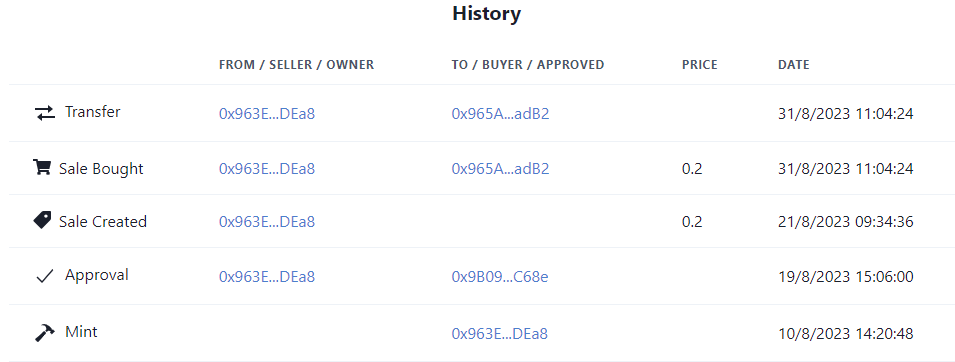
\includegraphics[width=\textwidth]{images/result_history.png}}
    \caption{Storico delle transazioni di un asset}
    \label{fig:risultati_storico}
\end{figure}

\begin{figure}[H]
    \centering
    \fcolorbox{mint-cream}{white}{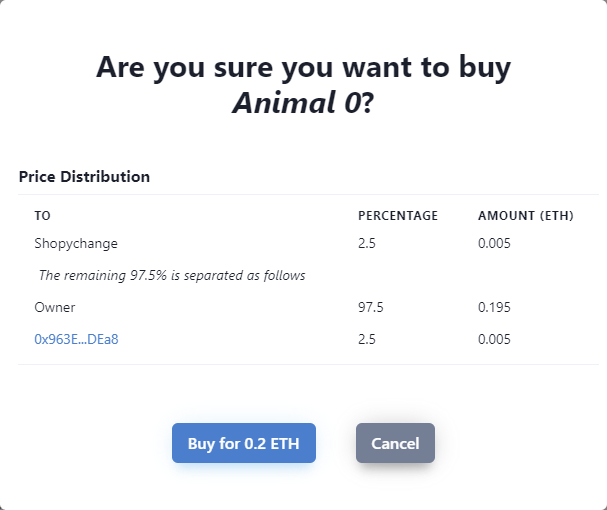
\includegraphics[width=0.6\textwidth]{images/result_royalty.png}}
    \caption{Divisione delle \textit{royalties} all'acquisto di un asset}  
    \label{fig:risulati_royalty}
\end{figure}

In aggiunta, sono in corso di sviluppo importanti funzionalità all'interno dei mercati decentralizzati, come ad esempio la possibilità di \textit{tokenizzare} beni fisici, come vestiti ed accessori, per poterli vendere in un ambiente decentralizzato. Ne è un esempio il progetto del famoso marchio \textit{Zara}, il quale ha lanciato una collezione di abiti \textit{NFT} che presentano la controparte fisica.  Questo concetto è estendibile ad un qualsiasi bene materiale, come ad esempio un'automobile o un immobile. \cite{belk2022money} Così facendo la società odierna risulterebbe essere più autonoma nelle transazioni commerciali, senza la necessità di intermediari ma con la possibilità di avere un ambiente sicuro e trasparente per portare a termine una trattativa. Il problema del concetto di \textit{tokenizzazione} risiede nell'effettivo trasferimento fisico del bene. 

Inoltre, in una situazione ipotetica potrebbe essere aggiunta la possibilità di frazionare la proprietà di un bene. Quest'ultima funzionalità risulterebbe utile nel concetto di \textit{revenue share}; il creatore possiederebbe una quota di proprietà, la quale aumenterebbe ad ogni rivendita, in modo da garantire un guadagno continuo in base al successo del bene. 

Tuttavia queste funzionalità sarebbero vane se non usufruite da un numero sufficiente di utenti. Personalmente trovo l'interfacciamento con la blockchain non adatto ad un utente medio, sarebbe necessaria una semplificazione dell'interazione con la blockchain per rendere la tecnologia più attrattiva agli utenti meno esperti. A tal proposito
sembrerebbe, infatti, che i \textit{GenZ} e i \textit{Millenials} (nati tra il 1980 e il 2012) siano più propensi alla detenzione di criptovalute rispetto alle generazioni precedenti. \cite{belk2022money}. Ciononostante sarebbe necessario un ulteriore studio per comprendere se questa tendenza è dovuta ad un interesse verso la tecnologia decentralizzata o semplicemente ad un fenomeno di \textit{FOMO} (\textit{Fear Of Missing Out}) a causa della forte volatilità del mercato. \cite{genz-fomo} 

Un altro aspetto da considerare è lo pseudonimato garantito dalla blockchain, il quale potrebbe portare ad un aumento di attività illecite.

\begin{figure}[H]
    \centering
    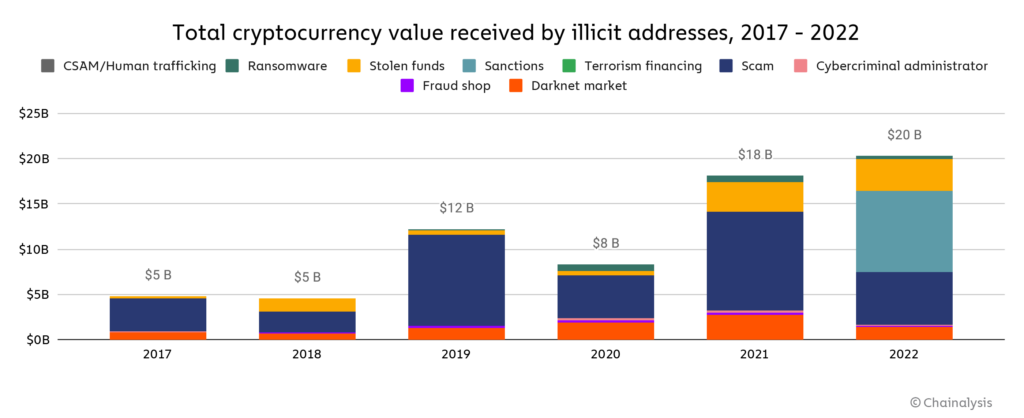
\includegraphics[width=\textwidth]{images/result_illecit.png}
    \caption{Attività illecite con criptovalute 2017 - 2022}  
    \label{fig:risultati_illecito}
\end{figure}

Come riportato dalle analisi di \textit{Chainalysis} \cite{chainalysis-money-laundering}, delle quali è possibile vedere un estratto in figura \ref{fig:risultati_illecito}, è stato riscontrato un incremento di attività illecite, in particolare di \textit{money laundering} attraverso l'uso delle principali criptovalute. Questo fenomeno è dovuto al fatto che, come spesso accade con tecnologie nuove, gli NFT offrono opportunità di abuso. Sebbene la tecnologia non è anonima ma pseudonima, ovvero non è possibile risalire all'identità di un utente ma è possibile ricostruire tutte le transazioni effettuate da un indirizzo, il che rappresenta comunque un problema per le autorità. \cite{bitstamp-privacy}

Concludendo, la tecnologia blockchain è uno strumento rivoluzionario che altererà il modo con il quale la società interagisce con i beni digitali e fisici. Tuttavia, sono necessari ulteriori sforzi implementativi e regolatori per rendere la tecnologia più accessibile e sicura.

% ***Problema***:
% - Eccessiva centralizzazione dei marketplace e troppa fiducia è riposta in essi


% ***Marketplace decentralizzato***: OK
% - Presenta degli enormi vantaggi rispetto a quello centralizzato. Es: sicurezza, privacy, controllo, censura, etc.


% - Gestione della tokenizzazione di un bene tangibile/fisico:
%  * https://www.vogue.com/article/zara-metaverse-collection, https://ww.fashionnetwork.com/news/Zara-returns-to-the-metaverse-with-zepeto,1515026.html


% - Money Laundering OK
%     *https://www.theverge.com/2022/2/2/22914056/nft-money-laundering-chainalysis
%     https://www.chainalysis.com/blog/2022-crypto-crime-report-preview-nft-wash-trading-money-laundering/


% - Troppo complesso per l'utente medio, usato da GenZ e Millenials OK
%     *https://dot.la/deloitte-gen-z-survey-2652644585.html
%     * https://www.fool.com/research/what-are-gen-z-millennial-investors-buying/
%     % * https://www.businessinsider.com/gen-z-are-investing-crypto-stocks-because-of-fomo-survey-2023-6?r=US&IR=T#:~:text=Redeem%20now-,Over%2040%25%20of%20Gen%20Z%20are%20investing%20because%20they're,and%20investing%20through%20social%20media.


% - La mancata regolarizzazione del mercato decentralizzato è un problema in quanto non si ha un controllo sulle transazioni e essendo anonime non si può risalire ai responsabili


\chapter{Conclusioni}

All'interno di questo capitolo verranno presentate le conclusioni del lavoro svolto, discutendo i risultati ottenuti, i problemi riscontrati e proponendo possibili sviluppi futuri.

Il progetto ha avuto come obiettivo la realizzazione di un marketplace decentralizzato per migliorare i processi di vendita, rendendoli più sicuri e trasparenti. Il lavoro svolto ha permesso di creare un luogo di scambio consono alle esigenze di creatori, venditori e acquirenti, senza la necessità di intermediari.

Come discusso nel capitolo \hyperref[sec:risultati]{\textit{Risultati}}, la tecnologia \textit{Blockchain} permette un approccio rivoluzionario allo scambio di beni, garantendo diverse migliorie rispetto ai sistemi tradizionali. Attualmente lo strumento sviluppato è adatto a diversi business, in particolare a quelli che necessitano una maggiore trasparenza e sicurezza. Alcuni esempi possono essere i mercati del gaming e dell'arte digitale. Ma con delle varianti, riguardanti il salvataggio dei metadati degli asset, il sistema potrebbe essere adatto anche per il settore di licenze su software, musica, video e molto altro. Negli ambiti appena citati il concetto di \textit{revenue share} risulterebbe fondamentale, in quanto permetterebbe di garantire un guadagno continuo ai creatori degli asset, anche dopo la vendita iniziale. Tuttavia, prevedo che la tecnologia \textit{Blockchain} migliorerà e si svilupperà ulteriormente per poter essere adottata su larga scala, con lo scopo di avere una maggior interoperabilità tra i diversi sistemi creati su di essa.

A livello professionale il progetto mi ha consentito di approfondire diverse conoscenze e di sviluppare nuove competenze. In particolare, ho avuto modo di migliorare le mie capacità di analisi, di progettazione e di sviluppo. Ho anche arricchito la mia capacità di affrontare situazioni decisionali e di effettuare ricerca scientifica. 

Il progetto ha favorito la mia crescita professionale, scaturita dal conseguimento di nuove competenze o dall'approfondimento di conoscenze ottenute durante il percorso di studi. In particolar modo grazie alle tecnologie e linguaggi utilizzati, ovvero \textit{React}, \textit{Solidity} e \textit{Python framework}.

\newpage

Sono soddisfatto del lavoro svolto e dei risultati ottenuti. Sono sicuro di aver contribuito alla realizzazione di un sistema che, un giorno, migliorerà l'approccio della società verso i beni digitali e fisici, attraverso un sistema equo e trasparente. Come disse Hal Finney: \footnote{Computer scientist e criptografo, è stato il primo destinatario di una transazione Bitcoin}

\begin{quote}
    \centering
\textit{"The computer can be used as a tool to liberate and protect people, rather than to control them"}
\end{quote}
    
\section{Problemi noti}

La soluzione proposta presenta un unico problema noto, ovvero la connessione tra un \textit{device} mobile ed un wallet. Come descritto nel capitolo \hyperref[sec:architettura]{\textit{Architettura}}, il problema è presumibilmente causato dal \textit{deep linking} tra più applicazioni. Una possibile soluzione è quella di includere un certificato all'interno dell'applicativo frontend, in modo da poter utilizzare il protocollo \textit{https}.

\section{Sviluppi futuri}

Gli sviluppi futuri potrebbero essere molteplici e toccare diversi aspetti del progetto. Di seguito sono elencate alcune funzionalità che potrebbero essere implementate:

\begin{itemize}
    \item Caching dei dati presenti nella blockchain, in modo da ridurre i tempi di risposta.
    \item Possibilità di concedere la gestione di un NFT ad un altro utente.
    \item Creazione di un sistema di asset preferiti.
    \item Barra di ricerca per il filtraggio degli asset.
    \item Creazione di una collezione di NFT con \textit{freeze}, ovvero la possibilità di non poter aggiungere asset alla collezione.
    \item Estendere in concetto di NFT ad asset che non siano unicamente immagini.
\end{itemize}





\printbibliography[title={Bibliografia},nottype=online]
\printbibliography[title={Linkografia},type=online]
\end{document}
